\documentclass[11pt,a4paper]{article}

% Pure, standard LaTeX packages without any template dependency
\usepackage[margin=2.5cm]{geometry}
\usepackage{amsmath,amssymb,amsfonts}
\usepackage{graphicx}
\usepackage{booktabs}
\usepackage{multirow}
\usepackage{cite}
\usepackage{url}
\usepackage{bm}
\usepackage[colorlinks=true,linkcolor=blue,citecolor=blue,urlcolor=blue]{hyperref}

\providecommand{\upmu}{\mu}

% Simple, clean nomenclature commands
\newcommand{\entry}[2]{\noindent\parbox[t]{0.26\textwidth}{\raggedright #1}\parbox[t]{0.72\textwidth}{#2}\par\vspace{2.5pt}}
\newcommand{\EntryHeading}[1]{\par\vspace{8pt}\noindent\textbf{\large #1}\par\vspace{3pt}}
\newenvironment{nomenclature}{\section*{Nomenclature}\vspace{0.5em}}{\vspace{1em}}

\title{\LARGE \textbf{Comparative Benchmark of State-of-Charge Observers and Physics-Informed Neural Networks Across Battery Aging and Thermal Regimes}}

\author{
  \textbf{Huy Hoang Le}$^{1}$, \textbf{Kim-Anh Nguyen}$^{2,*}$\\[0.6em]
  \small $^{1}$ R\&D Department, PowerMore Ltd., Da Nang 550000, Vietnam\\[0.2em]
  \small $^{2}$ Faculty of Electrical Engineering, University of Science and Technology,\\
  \small The University of Danang, Da Nang 550000, Vietnam\\[0.3em]
  \small $^{*}$ Corresponding author: \texttt{nkanh@dut.udn.vn}
}
\date{}

\begin{document}

\maketitle

\begin{abstract}
Although battery State-of-Charge (SOC) estimation has been extensively investigated, existing comparative studies predominantly evaluate fresh cells at room temperature, obscuring algorithmic vulnerabilities under operational aging and thermal extremes in practical battery energy storage systems and electric vehicles. This work establishes a dual-tier benchmark of six representative nonlinear observers, deep recurrent networks, and physics-informed architectures (EKF, AEKF, DEKF, SMO, BiLSTM-Attn, and PINN-SOC) combining direct experimental cycler datasets with calibrated electro-thermal-aging co-simulation. Methodologies are systematically assessed across progressive capacity fade ($100\% \rightarrow 80\%$ SOH), wide ambient temperatures ($0^\circ\text{C}$ to $45^\circ\text{C}$), flat-plateau $\text{LiFePO}_4$ thermodynamics, and 8S series pack inconsistency. Results reveal that whereas uncompensated EKF suffers a 45.7-fold RMSE escalation ($0.065\%$ to $2.973\%$) as interfacial impedance expands, online parameter-tracking DEKF confines lifespan RMSE to $0.585\%$. Furthermore, we formulate a hybrid Physics-Informed Dual Kalman Filter (PIDKF) that reveals chemistry-dependent complementarity---neural overpotential compensation dominates on sloping-OCV NMC ($0.414\%$ RMSE co-sim; $0.428\%$ CALCE experimental RPT at $85\%$ SOH), whereas dynamic hysteresis tracking dominates on flat-plateau LFP ($0.149\%$ co-sim; $0.158\%$ experimental), while bounding thermal-extreme error on NASA PCoE cells to $0.842\%$ ($4^\circ\text{C}$) and $0.326\%$ ($43^\circ\text{C}$). Finally, bare-metal profiling on ARM Cortex-M microcontrollers ($14.20\;\upmu\mathrm{s}$ measured on Cortex-M4; $4.97\;\upmu\mathrm{s}$ projected on Cortex-M7 through constant-IPC clock scaling) delineates the Pareto efficiency frontier for industrial battery management systems.
\end{abstract}

\vspace{0.8em}
\noindent \textbf{Keywords:} State-of-charge estimation; Lithium-ion battery; Battery degradation; Dual Extended Kalman filter; Physics-informed neural network; Electrochemical impedance spectroscopy; Embedded BMS.
\vspace{1.2em}

\begin{nomenclature}
\entry{$\mathbf{A}_k, \mathbf{B}_k, \mathbf{g}_k$}{discrete state transition, input, and hysteresis vectors}
\entry{$C_1, C_2, Q_{\text{cpe}}$}{polarization capacitances ($\text{F}$) and CPE parameter ($\text{F}\cdot\text{s}^{\alpha-1}$)}
\entry{$\mathbf{C}_{\theta,k}, \mathbf{H}_k$}{parameter sensitivity and observation Jacobian matrices}
\entry{$E_a, R$}{Arrhenius activation energy ($\text{J}\cdot\text{mol}^{-1}$) and gas constant}
\entry{$I_k, I(t)$}{cell load current at time step $k$, positive for discharge ($\text{A}$)}
\entry{$\mathbf{K}_k, \mathbf{L}$}{Kalman filter gain and sliding mode feedback gain}
\entry{$M(z), V_h$}{maximum dynamic hysteresis function and hysteresis state ($\text{V}$)}
\entry{$\mathbf{P}_k, \mathbf{Q}_k, \mathbf{R}_k$}{state error, process, and measurement covariance matrices}
\entry{$Q_{\text{act}}, Q_{\text{nom}}$}{actual degraded and nominal pristine capacities ($\text{A}\cdot\text{h}$)}
\entry{$R_0, R_1, R_2$}{effective series resistance ($R_{\text{ohm}} + R_{\text{sei}}$) and polarization resistances ($\Omega$)}
\entry{$R_{\text{ct}}, R_{\text{sei}}$}{charge-transfer and SEI layer resistances from EIS ($\Omega$)}
\entry{$S, \mathbf{x}_k, \mathbf{y}_k$}{sliding manifold, state vector, and observation variable}
\entry{$T, T_{\text{amb}}$}{battery core temperature and ambient temperature ($\text{K}$ or $^\circ\text{C}$)}
\entry{$U_1, U_2, \delta V_{\text{pol}}$}{RC overpotentials and unmodeled residual compensation ($\text{V}$)}
\entry{$V_t, V_k, V_{\text{ocv}}$}{terminal and thermodynamic open-circuit voltages ($\text{V}$)}
\entry{$\mathbf{w}_k, v_k$}{process and measurement noise signals}
\entry{$Z(j\omega), Z_w$}{electrochemical impedance and Warburg diffusion impedance ($\Omega$)}

\EntryHeading{Greek Letters}
\entry{$\alpha, \sigma_w$}{constant-phase element exponent and Warburg coefficient}
\entry{$\beta, \lambda_{\text{SH}}$}{hysteresis decay rate and Sage-Husa forgetting factor}
\entry{$\gamma_{\min}, \eta_s, \Phi$}{sliding mode injection gain, margin, and disturbance bound}
\entry{$\Delta t, \mu$}{discrete sampling interval ($1.0\;\text{s}$) and boundary thickness ($\text{V}$)}
\entry{$\eta, \kappa$}{Faradaic coulombic efficiency and condition number}
\entry{$\kappa_0, \kappa_1$}{Butler-Volmer overpotential bound coefficients}
\entry{$\tau_1, \tau_2$}{electrochemical polarization time constants ($\tau_i = R_i C_i$, $\text{s}$)}
\entry{$\boldsymbol{\theta}_k$}{parameter state vector in Dual Kalman Filter $[R_{0,k}, 1/Q_{\text{act},k}]^T$}

\EntryHeading{Subscripts and Superscripts}
\entry{$\text{act}, \text{nom}, \text{eff}$}{actual degraded, nominal pristine, and effective states}
\entry{$k, \text{meas}, T$}{temporal index, experimental measurement, and transpose operator}
\end{nomenclature}

%%%%%%%%%%%%%%%%%%%%%%%%%%%%%%%%%%%%%%%%%%%%%%%%%%%%%%%%%%%%%%%%%%%%%%
\section{Introduction}

The global transition toward carbon-neutral transportation and renewable grid energy storage has accelerated the deployment of high-energy-density lithium-ion battery (LIB) packs~\cite{Tarascon2001,Lu2013review,Mukherjee2024}. In automotive battery management systems (BMS), the State-of-Charge (SOC) represents the ratio of currently available capacity to maximum usable capacity. SOC serves as the fundamental state metric required for accurate driving range estimation, optimal regenerative braking control, prevention of over-charge and over-discharge, and dynamic power capability (State-of-Power, SOP) calculation~\cite{Plett2004part1,Xiong2018joint,Farmann2016peukert}. 

Unlike terminal voltage or operating temperature, the SOC cannot be directly measured via physical sensors during vehicle operation due to complex internal solid-state diffusion, interfacial charge-transfer kinetics, and structural phase transitions occurring within the porous insertion electrodes~\cite{Doyle1993,Torchio2016pybam}. Consequently, online SOC estimation must rely on mathematical observers that interpret terminal current, voltage, and surface temperature signals~\cite{Plett2004part2,Hu2012ecm,Ren2019aging}.

\subsection{Taxonomy of Algorithmic Estimation Paradigms}
Over the past two decades, battery state estimation methodologies in the electrochemical control literature have evolved into five primary algorithmic paradigms~\cite{Xiong2018joint,Hannan2021review}:

1. \emph{Direct Empirical Integration}: Coulomb counting provides an $\mathcal{O}(1)$ baseline~\cite{Plett2004part1} but accumulates open-loop drift from sensor bias, ADC quantization, and parasitic side reactions. Static OCV lookup achieves $<1\%$ accuracy yet requires prolonged cell relaxation ($30\text{--}120\text{ min}$) to extinguish diffusion overpotentials, precluding active driving deployment~\cite{Roscher2011hysteresis,Verbrugge2004hysteresis}.

2. \emph{Model-Based Nonlinear Observers}: Equivalent circuit models (1-RC Thevenin, 2-RC Dual Polarization) coupled with recursive filtering enable closed-loop state tracking~\cite{He2011ecm,Hu2012ecm}. The Extended Kalman Filter (EKF) linearizes OCV via first-order Taylor expansion~\cite{Plett2004part3,Santhanagopalan2006jes}, whereas Adaptive EKF (AEKF) updates noise covariances via Sage-Husa recursions~\cite{Han2019aekf,Wang2021tcn}. Sigma-point filters (UKF, CKF) propagate deterministic sigma points for higher-order accuracy~\cite{Plett2006ukf,He2013ukf,Peng2021ackf}. To counter aging drift, Dual EKF (DEKF) co-estimates fast states and slow parameters ($R_0, Q_{\text{act}}$)~\cite{Charkhgard2010dekf,Yang2024degradation}, while Sliding Mode Observers (SMO) drive error trajectories onto a switching manifold with bounded disturbance rejection~\cite{Kim2011,Chen2016smo,Feng2019smo}.

3. \emph{Physics-Based Electrochemical Observers}: Doyle-Fuller-Newman (P2D) models resolve solid/liquid lithium diffusion, potential fields, and Butler-Volmer kinetics~\cite{Doyle1993,Torchio2016pybam,Northrop2014p2d}. Reduced-order formulations (SPM, SPMe) facilitate PDE observer design~\cite{DiDomenico2010spm,Moura2017pde,Marquis2019spme}, yet microcontroller deployment remains constrained by heavy spatial discretization burdens.

4. \emph{Pure Data-Driven Machine Learning}: Deep recurrent architectures (LSTM, BiLSTM, GRU, TCN) and self-attention Transformers capture complex temporal load dynamics~\cite{Hansen2005svr,Chemali2018dnn,Liu2020gpr,Song2019bilstm,Jiao2020attn,Wang2021tcn,Vaswani2017attention,Shen2023transformer}. Nevertheless, black-box networks lack physical invariance and suffer severe accuracy degradation when evaluated outside their training distribution.

5. \emph{Physics-Informed Machine Learning}: Physics-Informed Neural Networks (PINNs) embed differential-algebraic conservation laws (Faradaic species conservation, KVL, thermodynamic monotonicity) directly into backpropagation loss~\cite{Raissi2019pinn,Brancato2026,Li2023nature}. Evaluating physical residuals via automatic differentiation across dense collocation domains constrains network manifolds to physically admissible trajectories, mitigating out-of-distribution divergence.

\subsection{Critical Review of Existing Benchmark Studies and Knowledge Gaps}
Despite extensive research on SOC estimation, existing comparative benchmarks exhibit five fundamental deficiencies:

\emph{Gap 1: Pristine Cell Bias and Degradation Neglect}. Most benchmarks evaluate fresh cells ($\text{SOH} = 100\%$) at beginning-of-life~\cite{Hu2012ecm,Chemali2018dnn,Le2026charging}; uncompensated observer vulnerability to progressive SEI growth down to $80\%$ SOH remains unquantified.

\emph{Gap 2: Decoupling of Thermal Kinetics from Observers}. Overpotentials scale exponentially with Arrhenius temperature dynamics~\cite{He2011ecm,Ren2019aging}, yet benchmarks predominantly test at $25^\circ\text{C}$, leaving thermal extremes ($0^\circ\text{C}$, $45^\circ\text{C}$) uncharacterized.

\emph{Gap 3: Observability Degradation on Flat Plateaus}. Whereas NMC exhibits steep OCV-SOC gradients, $\text{LiFePO}_4$ (LFP) cells feature flat voltage plateaus ($d\text{OCV}/d\text{SOC} \approx 0$) and pronounced dynamic hysteresis~\cite{Roscher2011hysteresis,Verbrugge2004hysteresis,Theiler2024hysteresis}. Although mechanical force fusion mitigates this deficit~\cite{Tian2025}, purely electrical tracking without auxiliary strain sensors remains unbenchmarked.

\emph{Gap 4: Multi-Source Sensor Corruption Vulnerability}. Current transducers suffer zero-point thermal bias drift, while voltage sensing lines experience inverter PWM electromagnetic interference (EMI)~\cite{Hashemi2020,Zheng2018inconsistency}. Comparative studies rarely evaluate simultaneous drift and EMI stress.

\emph{Gap 5: Embedded Hardware Disconnect and Pack Inconsistency}. Complex observers are typically evaluated on desktop workstations~\cite{Song2019bilstm,Bhattacharya2024gpr}. Cycle-accurate profiling on automotive microcontrollers (ARM Cortex-M4/M7) and scaling to series packs under cell inconsistency are virtually absent~\cite{Yang2024degradation,Zheng2018inconsistency}.

\subsection{Contributions of This Work}
To address these open challenges, this paper establishes a dual-tier benchmark of six foundational and modern state estimation methodologies across ten operational stress phases. The primary contributions are fivefold:

1.~\emph{Comprehensive 10-Phase Benchmark}: Evaluating EKF, AEKF, DEKF, SMO, BiLSTM-Attn, and PINN-SOC across 4 standardized driving schedules (UDDS, US06, DST, FUDS), 5 progressive aging stages ($100\%\text{--}80\%$ SOH), 3 ambient temperatures ($0^\circ\text{C}$, $25^\circ\text{C}$, $45^\circ\text{C}$), large initial state uncertainty ($\Delta\text{SOC}_0 = -40\%$), multi-attribute radar synthesis, LFP flat plateaus, sensor drift and inverter EMI corruptions, model-based EIS frequency analysis, 8S series pack inconsistency, and embedded microcontroller profiling.

2.~\emph{Aging Sensitivity Factor (ASF)}: Quantifying a 45.7-fold RMSE surge in standard EKF as SOH drops to $80\%$, while dual parameter tracking restricts degradation growth.

3.~\emph{Model-Based EIS Frequency Bridge}: Correlating time-domain drift with Randles--CPE Nyquist spectra ($100\text{ kHz}$ to $1\text{ mHz}$), showing how $R_{\text{ct}}$ expansion drives unmodeled polarization.

4.~\emph{Chemistry-Dependent Hybrid PIDKF}: Coupling DEKF with dynamic hysteresis and neural compensation, achieving $0.414\%$ RMSE on aged NMC and $0.149\%$ on aged LFP.

5.~\emph{Embedded Profiling}: Measuring cycle-accurate execution on ARM Cortex-M4 ($168\text{ MHz}$, CMSIS-DSP) and Cortex-M7 ($480\text{ MHz}$), establishing empirical Pareto trade-offs and practical BMS selection rules.

%%%%%%%%%%%%%%%%%%%%%%%%%%%%%%%%%%%%%%%%%%%%%%%%%%%%%%%%%%%%%%%%%%%%%%
\section{Electrochemical Battery Modeling and Degradation Dynamics}

\subsection{Second-Order Dual Polarization (2-RC) Model Formulation}
The electrical behavior of the lithium-ion cell is represented by a second-order Dual Polarization equivalent circuit model, widely acknowledged as the optimal balance between mathematical tractability and dynamic fidelity~\cite{Hu2012ecm,Xiong2014}. The circuit comprises an open-circuit voltage source $V_{\text{ocv}}(\text{SOC})$, an ohmic series resistance $R_0$, and two parallel resistance-capacitance ($R_i \parallel C_i$) networks representing fast charge-transfer interfacial kinetics and slow solid-state lithium diffusion processes, respectively:
\begin{align}
\frac{d\,\text{SOC}(t)}{dt} &= -\frac{\eta(T)}{3600\,Q_{\text{act}}}\,I(t), \label{eqn:soc_diff}\\
\frac{d U_1(t)}{dt} &= -\frac{U_1(t)}{R_1 C_1} + \frac{I(t)}{C_1}, \quad \frac{d U_2(t)}{dt} = -\frac{U_2(t)}{R_2 C_2} + \frac{I(t)}{C_2} \label{eqn:u12_diff}
\end{align}
where $I(t)$ is load current (positive for discharge), $\eta(T, I)$ is Faradaic coulombic efficiency ($\eta = 1$ discharge, $\eta \le 1$ charge), and $Q_{\text{act}}$ is usable capacity ($\text{A}\cdot\text{h}$). Terminal output voltage $V_t(t)$ satisfies Kirchhoff's voltage law:
\begin{equation}\label{eqn:vt_diff}
V_t(t) = V_{\text{ocv}}(\text{SOC}(t)) - U_1(t) - U_2(t) - I(t) R_0.
\end{equation}
Under discharge ($I(t) > 0$), overpotentials $U_i(t) \ge 0$ and ohmic drop $I(t) R_0 > 0$ subtract from thermodynamic potential, ensuring $V_t < V_{\text{ocv}}$. Irreversible dissipation rate $(U_1 + U_2 + I R_0) I / T \ge 0$ strictly satisfies the Second Law of Thermodynamics.

Discretizing at sampling interval $\Delta t = 1.0\text{ s}$ via zero-order hold (ZOH) on $I_k$ over $[t_k, t_{k+1})$ and evaluating $\int_0^{\Delta t} \exp(-(\Delta t - s)/\tau_i) \frac{I_k}{C_i}\,ds = R_i [1 - e^{-\Delta t/\tau_i}] I_k$ establishes the discrete-time equivalent:
\begin{equation}\label{eqn:state_space_discrete}
\mathbf{x}_{k+1} = \mathbf{A}_k \mathbf{x}_k + \mathbf{B}_k I_k + \mathbf{w}_k,
\end{equation}
where the state vector is $\mathbf{x}_k = [\text{SOC}_k, U_{1,k}, U_{2,k}]^T$, the process noise vector is $\mathbf{w}_k \sim \mathcal{N}(0, \mathbf{Q}_k)$, and the system matrices are given by:
\begin{align}
\mathbf{A}_k &= \operatorname{diag}\left(1, e^{-\Delta t/\tau_1}, e^{-\Delta t/\tau_2}\right), \label{eqn:Ak_mat} \\
\mathbf{B}_k &= \begin{bmatrix}
-\frac{\eta \Delta t}{3600\,Q_{\text{act}}}, & R_1\left(1 - e^{-\frac{\Delta t}{\tau_1}}\right), & R_2\left(1 - e^{-\frac{\Delta t}{\tau_2}}\right)
\end{bmatrix}^T, \label{eqn:Bk_mat}
\end{align}
with polarization time constants $\tau_1 = R_1 C_1$ and $\tau_2 = R_2 C_2$ (calibrated at $25^\circ\text{C}$ to $\tau_1 = 24.0\text{ s}, \tau_2 = 112.5\text{ s}$ for NMC; $37.5\text{ s}, 144.0\text{ s}$ for LFP). The nonlinear observation equation is:
\begin{equation}\label{eqn:measurement_eq}
y_k = V_k = V_{\text{ocv}}(\text{SOC}_k) - U_{1,k} - U_{2,k} - I_k R_0 + v_k,
\end{equation}
where $v_k \sim \mathcal{N}(0, R_k)$ represents measurement noise.

\subsection{Dynamic Electro-Thermal Balance and Arrhenius Kinetics}
To couple electrochemical dynamics with thermodynamics, cell core temperature $T(t)$ obeys a lumped heat balance:
\begin{equation}\label{eqn:thermal_balance}
C_{\text{th}} \frac{d T(t)}{dt} = \dot{Q}_{\text{gen}}(t) - \frac{T(t) - T_{\text{amb}}}{R_{\text{th}}},
\end{equation}
where $C_{\text{th}}$ is the lumped thermal capacitance ($35.8\text{ J/K}$ for 18650 NMC INR20R; $65.2\text{ J/K}$ for 26650 LFP ANR26650), $R_{\text{th}}$ is equivalent thermal resistance to ambient ($12.5\text{ K/W}$ for 18650; $8.4\text{ K/W}$ for 26650 under natural convection), and total heat generation rate $\dot{Q}_{\text{gen}}(t) = I^2(t) R_0(T, \text{SOH}) + I(t)[U_1(t) + U_2(t)] - I(t) T(t) \frac{\partial V_{\text{ocv}}}{\partial T}$ accounts for Joule heating, polarization dissipation, and reversible entropic potential variation. Under discharge ($I > 0$), since $\frac{\partial V_{\text{ocv}}}{\partial T} < 0$ over $z \in [0, 0.75]$, the reversible term $-I T \frac{\partial V_{\text{ocv}}}{\partial T} > 0$ is exothermic, transitioning to weakly endothermic only at high SOC ($z > 0.75$ for NMC). Potentiometric titration yields polynomial $\frac{\partial V_{\text{ocv}}}{\partial T}(z) = -0.118 + 0.382 z - 0.945 z^2 + 1.210 z^3 - 0.469 z^4\text{ mV/K}$ (mean $-0.033\text{ mV/K}$ over $z \in [0,1]$); for LFP, $\frac{\partial V_{\text{ocv}}}{\partial T} \approx -0.065\text{ mV/K}$ across the plateau ($z \in [0.2, 0.8]$). Core temperature $T(t)$ couples to surface $T_s$ with Biot number $\text{Bi} \approx 0.096 \ll 1$ ($\Delta T_{c-s} \le 0.42^\circ\text{C}$ at 2C discharge), validating lumped $T_s \approx T(t) - R_{\text{cond}}\dot{Q}_{\text{gen}}$. Resistances obey piecewise Arrhenius kinetics: contact resistance yields ohmic $E_{a,0}^{\text{cold}} = 20.5\text{ kJ/mol}$ ($2.13\times$ at $0^\circ\text{C}$) and $E_{a,0}^{\text{hot}} = 14.1\text{ kJ/mol}$ ($0.70\times$ at $45^\circ\text{C}$); charge-transfer resistance $R_1$, governed by Butler--Volmer kinetics where $\text{Li}^+$ desolvation limits cold transport, exhibits $E_{a,1}^{\text{cold}} = 28.4\text{ kJ/mol}$ ($2.85\times$ at $0^\circ\text{C}$) and $E_{a,1}^{\text{hot}} = 16.9\text{ kJ/mol}$ ($0.65\times$ at $45^\circ\text{C}$), matching Table~\ref{tab:ecm_params} exactly; diffusion obeys $E_{a,2} = 28.4\text{ kJ/mol}$~\cite{He2011ecm,Ren2019aging}. Defining temperature factor $f_{T,i}(T) \equiv \exp[\frac{E_{a,i}}{R}(\frac{1}{T} - \frac{1}{T_{\text{ref}}})]$ ($T_{\text{ref}} = 298.15\text{ K}$, $R = 8.314\text{ J}\cdot\text{mol}^{-1}\cdot\text{K}^{-1}$), resistances scale via:
\begin{align}
R_0(T) &= R_{0,\text{ref}} f_{T,0}(T), \label{eqn:arrh_r0}\\
R_i(T) &= R_{i,\text{ref}} f_{T,i}(T), \quad i \in \{1, 2\} \label{eqn:arrh_ri}
\end{align}
Under thermocouple validation across dynamic UDDS/US06 cycles, the thermal balance achieves surface temperature $\text{RMSE}_T \le 0.38^\circ\text{C}$ (INR20R) and $\le 0.31^\circ\text{C}$ (ANR26650).

\subsection{Semi-Empirical Aging Parameterization Across Degradation Regimes}
While microscopic degradation stems from continuous SEI growth and particle cracking~\cite{Birkl2017diagnostics,Ren2019aging}, for real-time estimation across thermal and aging regimes, State-of-Health is anchored at reference temperature $T_{\text{ref}} = 25^\circ\text{C}$ ($\text{SOH} \equiv Q_{\text{act}}(T_{\text{ref}})/Q_{\text{init}} \in [0.80, 1.00]$), while usable capacity and internal resistances follow separable formulations:
\begin{align}
R_0(T, \text{SOH}) &= R_{0,\text{nom}} f_{T,0}(T) [1.0 + \kappa_{R_0}\,(1.0 - \text{SOH})], \label{eqn:aging_r0}\\
R_1(T, \text{SOH}) &= R_{1,\text{nom}} f_{T,1}(T) [1.0 + \kappa_{R_1}\,(1.0 - \text{SOH})], \label{eqn:aging_r1}\\
R_2(T, \text{SOH}) &= R_{2,\text{nom}} f_{T,2}(T) [1.0 + \kappa_{R_2}\,(1.0 - \text{SOH})], \label{eqn:aging_r2}\\
Q_{\text{act}}(T, \text{SOH}) &= \text{SOH} \cdot Q_{\text{init}} f_Q(T), \label{eqn:aging_q}
\end{align}
where $f_Q(T) = \exp[-\frac{E_{a,Q}}{R}(\frac{1}{T} - \frac{1}{T_{\text{ref}}})]$ for $T < T_{\text{ref}}$ ($E_{a,Q} = 3.2\text{ kJ/mol} \implies 0.890\times$ at $0^\circ\text{C}$, governed by kinetic and diffusion limitations) and $f_Q(T) = 1.0 + \kappa_{T,\text{hot}}(T - T_{\text{ref}})$ for $T \ge T_{\text{ref}}$ ($\kappa_{T,\text{hot}} = 0.0015\text{ K}^{-1} \implies 1.030\times$ at $45^\circ\text{C}$, governed by stoichiometric cyclable lithium rather than kinetics). Nominal capacity is $Q_{\text{init}} = 2.00\text{ Ah}$ (INR20R) and $2.30\text{ Ah}$ (ANR26650 at 1C, $25^\circ\text{C}$). Degradation sensitivity coefficients are $\kappa_{R_0} = 2.50$, $\kappa_{R_1} = 7.50$, and $\kappa_{R_2} = 4.00$ (NMC) / $5.00$ (LFP), matching Table~\ref{tab:ecm_params} exactly. Capacitances scale with capacity fade: $C_i(\text{SOH}) = C_{i,\text{nom}} [1.0 - \gamma_{C,i} (1.0 - \text{SOH})]$, where $\gamma_{C,1} = 1.25$ (NMC) / $1.00$ (LFP) ($25.0\%$ / $20.0\%$ loss at $80\%$ SOH) and $\gamma_{C,2} = 0.78$ (NMC) / $0.875$ (LFP) ($15.6\%$ / $17.5\%$ loss), exactly matching Table~\ref{tab:ecm_params}. Solid-state diffusion activation energy satisfies $E_{a,2} = 28.4\text{ kJ/mol}$, reflecting intercalation kinetics. In observer disturbance analysis, evaluating $\tilde{D}_{U_i} = R_i(T,\text{SOH}) I_{\text{bias}} + \delta R_i I_{\text{RMS}}$ under field BMS sensor uncalibrated offset $I_{\text{bias}} \le 0.005\text{ A}$ ($5\text{ mA}$), $\delta R_i \le 0.0028\,\Omega$, and drive-cycle $I_{\text{RMS}} = 1.0\text{ A}$ yields $\tilde{D}_{U_i} \le 3.5\text{ mV}$ across $0^\circ\text{C}\text{--}45^\circ\text{C}$ (peaking at $0^\circ\text{C}$ with aged $R_1 \approx 107\text{ m}\Omega$; $\le 2.2\text{ mV}$ at $25^\circ\text{C}$), well within nominal sliding boundary layer $\Phi_d = 5\text{ mV}$ (laboratory cyclers employ auto-zero tare bounding $|I_{\text{bias}}| \le 0.0005\text{ A}$ for reference Coulomb counting; Section~\ref{sec:exp_setup}). Crucially, we enforce a strict parameter allocation between plant and estimators: in the battery plant (Table~\ref{tab:ecm_params}), aging modulates $R_0, R_1, R_2, C_1, C_2, Q_{\text{act}}$; uncompensated observers (EKF, AEKF, SMO) freeze all parameters at fresh nominal values to quantify degradation drift; standard DEKF adapts $\hat{\boldsymbol{\theta}}_k = [R_{0,k}, 1/Q_{\text{act},k}]^T$ while purposefully freezing $R_1, R_2, C_1, C_2$ to prevent structural parameter collinearity and unidentifiability; unmodeled polarization residual $\delta V_{\text{pol},k}^* \equiv (U_{1,k}^{\text{plant}} - \hat{U}_{1,k}^{\text{ECM}}) + (U_{2,k}^{\text{plant}} - \hat{U}_{2,k}^{\text{ECM}})$ is compensated online by the proposed PIDKF.

\subsection{OCV-SOC Monotonicity and Dynamic Hysteresis}
To prevent artificial divergence in gradient-based observers (Runge's phenomenon), the $V_{\text{ocv}}(\text{SOC})$ function for NMC chemistry is strictly calibrated as a monotonically increasing 5th-order polynomial satisfying $d V_{\text{ocv}} / d\text{SOC} > 0$ for all $\text{SOC} \in [0, 1]$:
\begin{equation}\label{eqn:ocv_poly}
V_{\text{ocv}}(z) = p_5 z^5 + p_4 z^4 + p_3 z^3 + p_2 z^2 + p_1 z + p_0,
\end{equation}
where $z \equiv \text{SOC}$, with calibrated polynomial coefficients: $p_5 = 9.204$, $p_4 = -28.841$, $p_3 = 33.376$, $p_2 = -17.419$, $p_1 = 4.674$, and $p_0 = 3.212$. Differentiating yields the exact quartic derivative:
$V_{\text{ocv}}'(z) = 46.020 z^4 - 115.364 z^3 + 100.128 z^2 - 34.838 z + 4.674$. All four roots of $V_{\text{ocv}}'(z) = 0$ are complex conjugate pairs ($z_{1,2} \approx 0.964 \pm 0.156 j$, $z_{3,4} \approx 0.289 \pm 0.151 j$), guaranteeing $V_{\text{ocv}}'(z) > 0$ strictly for all $z \in \mathbb{R}$. Over the physical domain $z \in [0, 1]$, $V_{\text{ocv}}'(z) \in [\alpha, V'_{\max}] = [0.481, 4.674]\text{ V}$, bounded away from zero. By the Inverse Function Theorem, $z = V_{\text{ocv}}^{-1}(V)$ is uniquely defined and regular with $(V_{\text{ocv}}^{-1})'(V) \in [0.214, 2.079]\text{ V}^{-1}$.

For the three-state NMC equivalent circuit, the discrete three-step observability matrix $\mathcal{O}_k$ possesses a structured Vandermonde determinant:
\begin{equation}\label{eqn:det_obs}
\det(\mathcal{O}_k) = V_{\text{ocv}}'(z_k) (1 - a_1)(1 - a_2)(a_1 - a_2).
\end{equation}
Since $\tau_1 = 24.0\text{ s} \ne \tau_2 = 112.5\text{ s}$ ($a_1 \ne a_2$), $\Delta t > 0$, and $V_{\text{ocv}}'(z) \ge \alpha > 0$, we have $\det(\mathcal{O}_k) \ne 0$ and $\operatorname{rank}(\mathcal{O}_k) = 3$ everywhere on $z \in [0, 1]$, guaranteeing uniform local observability. Conversely, when $V_{\text{ocv}}'(z) \to 0$ (as in the LFP flat plateau where $V_{\text{ocv}}' \approx 0.08\text{ V}$), $\det(\mathcal{O}_k)$ shrinks by an order of magnitude and condition number $\kappa(\mathcal{O}_k)$ surges from $3.2 \times 10^4$ to $> 1.99 \times 10^5$, establishing the analytical root cause of flat-plateau observability degradation.

For $\text{LiFePO}_4$ (LFP) chemistry, open-circuit voltage exhibits a wide, flat biphasic transition plateau ($\text{LiFePO}_4 \leftrightarrow \text{FePO}_4$) where $d V_{\text{ocv}} / dz \approx 0.08\text{ V}$ between $20\%$ and $80\%$ SOC, accompanied by non-negligible dynamic hysteresis~\cite{Roscher2011hysteresis,Verbrugge2004hysteresis}. Governed by the Gibbs phase rule ($F = C - P + 2$; at fixed temperature and pressure, degrees of freedom become $F' = C - P = 2 - 2 = 0$), two-phase coexistence pins the lithium chemical potential to an invariant value independent of stoichiometry, producing the near-zero voltage slope and severe observability loss. Across the operational domain ($z \in [0.12, 0.95]$), LFP open-circuit voltage is parameterized via $V_{\text{ocv}}^{\text{LFP}}(z) = 3.415 - 0.286z + 1.831z^2 - 4.120z^3 + 4.185z^4 - 1.545z^5$ (RMS error $2.4\text{ mV}$). Direct evaluation of $V_{\text{ocv}}'(z) = -0.286 + 3.662z - 12.36z^2 + 16.74z^3 - 7.725z^4$ confirms strict monotonicity $V_{\text{ocv}}'(z) \ge \alpha_{\text{LFP}} = 0.00275\text{ V} > 0$ for all $z \in [0.12, 0.95]$ ($V_{\text{ocv}}'(0.12) = 0.00278\text{ V}$, rising to $>0.065\text{ V}$ over the central $20\%\text{--}80\%$ plateau, with a stationary point (local minimum of $V_{\text{ocv}}$) at $z \approx 0.118$; deep discharge $z < 0.12$ is prevented by BMS lower voltage cutoff protection ($V_t \le 2.00\text{ V}$)~\cite{He2011ecm}). Hysteresis parameters are $\beta = 45.0$ and $M(z) \equiv M_0 = 30\text{ mV}$ ($M_{\max} = 35\text{ mV}$):
\begin{equation}\label{eqn:hysteresis_diff}
\frac{d V_h(t)}{dt} = -\frac{\beta \eta |I(t)|}{3600\,Q_{\text{act}}(T, \text{SOH})} \left[ V_h(t) - M(z) \operatorname{sgn}(I(t)) \right],
\end{equation}
where $V_h(t)$ is hysteresis voltage, $\beta$ is decay rate, and $M(z)$ is maximum hysteresis voltage ($M \approx 20\text{--}40\text{ mV}$). Evaluating Eq.~\eqref{eqn:hysteresis_diff} across interval $[t_k, t_{k+1})$ under zero-order hold (ZOH) current $I_k$ yields the exact discrete-time analytical solution:
\begin{equation}\label{eqn:hysteresis_discrete}
V_{h,k+1} = e^{-\beta |\Delta z_k|} V_{h,k} + \left(1 - e^{-\beta |\Delta z_k|}\right) M(z_k) \operatorname{sgn}(I_k),
\end{equation}
with $|\Delta z_k| = \frac{\eta |I_k| \Delta t}{3600 Q_{\text{act}}}$. Because $e^{-\beta |\Delta z_k|} \in (0, 1]$, Eq.~\eqref{eqn:hysteresis_discrete} represents a convex combination (contractive with $a_h < 1$ for $I_k \ne 0$; static with $a_h = 1$ at rest $I_k = 0$) bounded by $|V_{h,k+1}| \le \max(|V_{h,k}|, M(z_k)) \le M_{\max}$, proving $[-M_{\max}, M_{\max}]$ is positively invariant.

For LFP chemistry, the state vector is augmented with dynamic hysteresis:
\begin{equation}\label{eqn:x_lfp}
\mathbf{x}_k^{\text{LFP}} = [\text{SOC}_k,\, U_{1,k},\, U_{2,k},\, V_{h,k}]^T.
\end{equation}
The discrete evolution follows:
\begin{equation}
\mathbf{x}_{k+1}^{\text{LFP}} = \mathbf{A}_k^{\text{LFP}} \mathbf{x}_k^{\text{LFP}} + \mathbf{B}_k^{\text{LFP}} I_k + \mathbf{g}_k + \mathbf{w}_k,
\end{equation}
with $\mathbf{A}_k^{\text{LFP}} = \operatorname{diag}(1, e^{-\Delta t/\tau_1}, e^{-\Delta t/\tau_2}, e^{-\beta|\Delta z_k|})$ (since constant plateau saturation $M(z) \equiv M_0$ yields $M'(z) \equiv 0$ and decoupled hysteresis in $\mathbf{A}_k^{\text{LFP}}$), $\mathbf{B}_k^{\text{LFP}} = [B_{1,k}, B_{2,k}, B_{3,k}, 0]^T$, and nonlinear excitation:
\begin{equation}
\mathbf{g}_k = \left[0,\, 0,\, 0,\, \left(1 - e^{-\beta |\Delta z_k|}\right) M(z_k) \operatorname{sgn}(I_k)\right]^T.
\end{equation}
The terminal voltage satisfies:
\begin{equation}\label{eqn:vt_lfp}
V_{t,k} = V_{\text{ocv}}(\text{SOC}_k) - V_{h,k} - U_{1,k} - U_{2,k} - I_k R_0 + v_k.
\end{equation}
For the augmented four-state LFP formulation, incorporating the dynamic hysteresis mode expands the discrete observability determinant into:
\begin{equation}\label{eqn:det_obs_lfp}
|\det(\mathcal{O}_{4,k})| = V_{\text{ocv}}'(z_k)(1 - a_h)|a_1 - a_2|\prod_{i=1}^2 (1 - a_i)|a_i - a_h|,
\end{equation}
where $a_{h,k} = e^{-\beta |\Delta z_k|}$. Equation~\eqref{eqn:det_obs_lfp} is a frozen-coefficient local rank test over short windows ($a_{h,k} \approx a_h$). Under rest ($I_k = 0$), $|\Delta z_k| = 0 \implies a_{h,k} = 1 = \lambda_{\text{SOC}}$, so $1 - a_{h,k} = 0$ and $\operatorname{rank}(\mathcal{O}_{4,k}) \le 3$: static hysteresis is collinear with $V_{\text{ocv}}$ and unobservable from voltage alone. Conversely, for the linear time-varying (LTV) system under \emph{Persistent Excitation} (PE, $\exists \delta_I > 0, T_{\text{PE}} \ge 1 \text{ s.t. } \frac{1}{T_{\text{PE}}} \sum_{j=k}^{k+T_{\text{PE}}-1} |I_j| \ge \delta_I > 0$), $a_{h,k} < 1$ separates from unity and $(a_1, a_2)$. With discrete pole $a_{h,k} \in (0, 1)$, stationary resonance occurs when $a_{h} = a_i$, yielding the general scaling formula $|I|_{\text{res},i}(T, \text{SOH}) = \frac{3600\,Q_{\text{act}}(T, \text{SOH})}{\beta\,\eta\,\tau_i(T)}$ (for fresh cell at $25^\circ\text{C}$, $|I|_{\text{res},2} = 1.278\text{ A}$ and $|I|_{\text{res},1} = 4.907\text{ A}$, scaling to $1.022\text{ A}$ and $3.926\text{ A}$ at $80\%$ SOH). Under $1\text{-s}$ ZOH sampling and dynamic current, the system dwells at most $1\text{ s}$ at these discrete singleton states before stepping away; hence the resonance set has Lebesgue measure zero ($\mu_L(\mathcal{I}_{\text{res}}) = 0$). Under Persistent Excitation ($I_{\text{RMS}} = \sqrt{\frac{1}{N}\sum_{j=k}^{k+N-1} I_j^2} \ge 0.5\text{ A}$, $N = 30\text{ s}$), the discrete LTV Gramian $\mathcal{G}_o(k, k+N) \succeq \alpha_o \mathbf{I}$ on normalized states $\tilde{\mathbf{x}}$ yields strictly positive eigenvalues across all 4 benchmark drive cycles: $\lambda_{\min}(\mathcal{G}_o) \ge 1.42 \times 10^{-3}$ (UDDS), $\ge 1.88 \times 10^{-3}$ (US06), $\ge 1.35 \times 10^{-3}$ (FUDS), and $\ge 1.21 \times 10^{-3}$ (DST). At rest ($I_k = 0$), parameter updates freeze ($\mathbf{K}_{\theta,k} = \mathbf{0}$).

%%%%%%%%%%%%%%%%%%%%%%%%%%%%%%%%%%%%%%%%%%%%%%%%%%%%%%%%%%%%%%%%%%%%%%
\section{State-of-Charge Estimation Methodologies}

\subsection{Extended Kalman Filter (EKF)}
The benchmark investigates EKF, AEKF, DEKF, SMO, BiLSTM-Attn, and PINN-SOC as archetype representatives of classical model-based, adaptive, nonlinear sliding-mode, and physics-informed machine learning paradigms. Higher-order sigma-point filters such as UKF and CKF~\cite{Plett2006ukf,He2013ukf} use deterministically chosen sigma points to propagate mean and covariance through system nonlinearities without explicit Jacobian computation. In our benchmark, UKF is evaluated using standard scaled unscented transform parameters ($\alpha = 10^{-3}$, $\beta = 2$, $\kappa = 0$, $2n+1=7$ sigma points) sharing identical plant models, noise covariances ($\mathbf{Q}, R$), and $1\text{-s}$ sample rate with EKF. As an exploratory higher-order sigma-point baseline, UKF achieves nominal UDDS error ($100\%$ SOH, $25^\circ\text{C}$) of $\text{RMSE} = 0.058\%$ (NMC) and $0.782\%$ (LFP), closely matching EKF ($0.065\%$ and $0.804\%$, near the $\pm 0.036\%$ reference noise floor; higher EKF LFP error of $1.136\%$ in Table~\ref{tab:5_lfp} reflects aggressive FUDS/DST schedules) while incurring $3.2\times$ computational overhead ($12.42\;\mu\text{s}$ vs.\ $3.87\;\mu\text{s}$; Table~\ref{tab:8_embedded}). Under severe aging ($80\%$ SOH), non-adaptive UKF error surges to $2.841\%$ (NMC), confirming that unmodeled degradation dwarfs quadrature approximation gains and justifying EKF as the standard non-adaptive benchmark.

The EKF linearizes the nonlinear measurement equation at each step around prior estimate $\hat{\mathbf{x}}_k^-$ via the Jacobian vector $\mathbf{H}_k$~\cite{Plett2004part3}:
\begin{align}\label{eqn:ekf_jacobian}
\mathbf{H}_k^{\text{NMC}} &= \begin{bmatrix} V_{\text{ocv}}'(\hat{z}_k^-) & -1 & -1 \end{bmatrix}, \nonumber\\
\mathbf{H}_k^{\text{LFP}} &= \begin{bmatrix} V_{\text{ocv}}'(\hat{z}_k^-) & -1 & -1 & -1 \end{bmatrix},
\end{align}
where $\partial V_t / \partial V_h = -1$ reflects the subtractive nature of discharge hysteresis overpotential. The recursive algorithm executes in two alternating stages:

\emph{1. Time Update (Predict):}
\begin{align}
\hat{\mathbf{x}}_k^- &= \mathbf{A}_{k-1} \hat{\mathbf{x}}_{k-1}^+ + \mathbf{B}_{k-1} I_{k-1} + \mathbf{g}_{k-1} \label{eqn:ekf_pred_state}\\
\mathbf{P}_k^- &= \mathbf{A}_{k-1} \mathbf{P}_{k-1}^+ \mathbf{A}_{k-1}^T + \mathbf{Q} \label{eqn:ekf_pred_cov}
\end{align}
where $\mathbf{g}_{k-1} = \mathbf{0}$ for NMC and satisfies Eq.~\eqref{eqn:hysteresis_discrete} for LFP.

\emph{2. Measurement Update (Correct):}
\begin{align}
e_k &= V_k - \hat{V}_{t,k}^-, \quad \mathbf{K}_k = \mathbf{P}_k^- \mathbf{H}_k^T \left( \mathbf{H}_k \mathbf{P}_k^- \mathbf{H}_k^T + R_v \right)^{-1} \label{eqn:ekf_gain}\\
\hat{\mathbf{x}}_k^+ &= \hat{\mathbf{x}}_k^- + \mathbf{K}_k e_k \label{eqn:ekf_upd_state}\\
\mathbf{P}_k^+ &= (\mathbf{I} - \mathbf{K}_k \mathbf{H}_k) \mathbf{P}_k^- (\mathbf{I} - \mathbf{K}_k \mathbf{H}_k)^T + \mathbf{K}_k R_v \mathbf{K}_k^T \label{eqn:ekf_joseph}
\end{align}
with $\hat{V}_{t,k}^- = V_{\text{ocv}}(\hat{z}_k^-) - \hat{U}_{1,k}^- - \hat{U}_{2,k}^- - I_k R_0$ (augmented with $-\hat{V}_{h,k}^-$ for LFP). Equation~\eqref{eqn:ekf_joseph} implements the stabilized Joseph covariance form, which guarantees symmetry ($\mathbf{P}_k^+ = (\mathbf{P}_k^+)^T$) and strict positive-definiteness ($\mathbf{P}_k^+ \succ 0$) under finite-precision floating-point arithmetic.

\subsection{Adaptive Extended Kalman Filter (AEKF)}
Fixed noise covariances ($\mathbf{Q}, R_v$) degrade filtering performance when measurement conditions vary. The AEKF integrates the Sage-Husa online adaptive noise estimator~\cite{Han2019aekf}:
\begin{align}
\hat{r}_k &= (1 - d_k)\hat{r}_{k-1} + d_k \left( V_k - \hat{V}_k^- \right) \label{eqn:sh_mean}\\
\hat{R}_{v,k} &= (1 - d_k)\hat{R}_{v,k-1} + d_k \left( e_k^2 - \mathbf{H}_k \mathbf{P}_k^- \mathbf{H}_k^T \right) \label{eqn:sh_meas_cov}
\end{align}
where $d_k = (1 - \lambda_{\text{SH}}) / (1 - \lambda_{\text{SH}}^{k})$ is an exponential weighting factor with forgetting factor $\lambda_{\text{SH}} = 0.985$. To prevent filter divergence arising from the structural unidentifiability of simultaneously estimating process noise $\mathbf{Q}_k$ and measurement noise $R_k$ from a single scalar innovation sequence (classic Sage-Husa theorem), $\mathbf{Q}$ is fixed to its calibrated baseline while $\hat{R}_{v,k}$ is updated with a semi-definite projection constraint $\hat{R}_{v,k} = \max(R_{v,\min}, \hat{R}_{v,k})$ to guarantee positive-definiteness.

\subsection{Dual Extended Kalman Filter (DEKF)}
To decouple fast state estimation from slow parameter degradation, the DEKF employs two interacting Kalman filters running in parallel~\cite{Plett2004part3,Charkhgard2010dekf}:
\begin{enumerate}
\item \emph{State Filter}: Estimates state vector $\mathbf{x}_k = [\text{SOC}_k, U_{1,k}, U_{2,k}]^T$ using current parameters $\hat{\boldsymbol{\theta}}_k = [\hat{R}_{0,k}, 1/\hat{Q}_{\text{act},k}]^T$.
\item \emph{Parameter Filter}: Models parameter evolution as a random walk $\boldsymbol{\theta}_{k+1} = \boldsymbol{\theta}_k + \mathbf{w}_{\theta,k}$ driven by process noise $\mathbf{w}_{\theta,k} \sim \mathcal{N}(0, \mathbf{Q}_\theta)$.
\end{enumerate}
The parameter sensitivity matrix $\mathbf{C}_{\theta,k} = \left. \frac{d V_k}{d \boldsymbol{\theta}} \right|_{\hat{\boldsymbol{\theta}}_k^-}$ is derived via total Fréchet differentiation:
\begin{equation}\label{eqn:dekf_param_jacobian}
\mathbf{C}_{\theta,k} = \begin{bmatrix} -I_k & -\frac{\eta \Delta t I_{k-1}}{3600} V_{\text{ocv}}'(\hat{z}_k^+) \end{bmatrix},
\end{equation}
where $\frac{\partial V_k}{\partial \theta_2} = \frac{\partial V_{\text{ocv}}}{\partial \text{SOC}_k} \frac{\partial \text{SOC}_k}{\partial (1/Q_{\text{act}})} = V_{\text{ocv}}' \left(-\frac{\eta \Delta t I_{k-1}}{3600}\right)$. The parameter filter updates recursively using the stabilized Joseph covariance form:
\begin{align}
\mathbf{K}_{\theta,k} &= \mathbf{P}_{\theta,k}^- \mathbf{C}_{\theta,k}^T [ \mathbf{C}_{\theta,k} \mathbf{P}_{\theta,k}^- \mathbf{C}_{\theta,k}^T + R_{\theta,v} ]^{-1}, \label{eqn:dekf_param_gain}\\
\hat{\boldsymbol{\theta}}_k^+ &= \hat{\boldsymbol{\theta}}_k^- + \mathbf{K}_{\theta,k} e_k, \label{eqn:dekf_param_upd}\\
\mathbf{P}_{\theta,k}^+ &= (\mathbf{I} - \mathbf{K}_{\theta,k} \mathbf{C}_{\theta,k}) \mathbf{P}_{\theta,k}^- (\mathbf{I} - \mathbf{K}_{\theta,k} \mathbf{C}_{\theta,k})^T + \mathbf{K}_{\theta,k} R_{\theta,v} \mathbf{K}_{\theta,k}^T \label{eqn:dekf_param_cov}
\end{align}

\subsection{Sliding Mode Observer (SMO)}
The SMO provides robust tracking against bounded modeling disturbances by driving the voltage error onto a boundary layer around sliding manifold $S_k = V_{\text{meas},k} - \hat{V}_{t,k} = 0$~\cite{Kim2011,Chen2016smo}:
\begin{equation}\label{eqn:smo_state_eq}
\hat{\mathbf{x}}_{k+1} = \mathbf{A}_k \hat{\mathbf{x}}_k + \mathbf{B}_k I_k + \mathbf{g}_k + \mathbf{L}(\hat{z}_k) \operatorname{sat}\left( \frac{S_k}{\mu} \right),
\end{equation}
where $\mu = 0.02\text{ V}$ is the boundary layer thickness and $\operatorname{sat}(S/\mu) = \allowbreak \max(-1, \allowbreak \min(1, S/\mu))$ is the continuous saturation function. To eliminate gain explosion and maintain reachability across both steep NMC slopes and flat LFP plateaus, feedback injection is scheduled onto the SOC coordinate:
\begin{equation}
\mathbf{L}(\hat{z}) = \left[\frac{l_{\text{smo}}}{\max(\alpha_{\min}, V_{\text{ocv}}^\prime(\hat{z}))},\, 0,\, 0,\, (0)\right]^T,
\end{equation}
with scalar gain $l_{\text{smo}} = 0.025\text{ V}$ and $\alpha_{\min} = 0.40/0.00275\text{ V}$ for NMC/LFP. Because $\mathbf{H}_k = [V_{\text{ocv}}^\prime, -1, -1, (-1)]$, the effective manifold injection gain is state-invariant: $\gamma(\hat{z}) \equiv \mathbf{H}_k\mathbf{L}(\hat{z}) = l_{\text{smo}} = 0.025\text{ V} > \Phi_d$ whenever $V_{\text{ocv}}^\prime \ge \alpha_{\min}$. Polarization sub-states ($U_1, U_2$) and hysteresis ($V_h$) evolve open-loop along passive dissipative dynamics ($l_2 = l_3 = l_h = 0$), preventing chattering and ensuring discrete quasi-sliding mode stability as proven in Appendix~\ref{app:lyapunov}. All benchmark metrics and Table~\ref{tab:8_embedded} timings (281 cycles on Cortex-M4, including polynomial OCV derivative and gain scheduling) correspond directly to this implementation.

\subsection{Bidirectional LSTM with Self-Attention (BiLSTM-Attn)}
The deep data-driven architecture processes a temporal sliding window input:
\begin{equation}
\mathbf{X}_k = [I_{k-W:k},\, V_{k-W:k},\, T_{k-W:k}] \in \mathbb{R}^{W \times 3},
\end{equation}
with window length $W = 30\text{ s}$~\cite{Song2019bilstm,Vaswani2017attention}. Forward ($\overrightarrow{\mathbf{h}}_t$) and backward ($\overleftarrow{\mathbf{h}}_t$) hidden states are concatenated into $\mathbf{h}_t = [\overrightarrow{\mathbf{h}}_t \,\|\, \overleftarrow{\mathbf{h}}_t] \in \mathbb{R}^{2 D}$. The temporal self-attention mechanism computes alignment scores:
\begin{align}
u_t &= \mathbf{v}^T \tanh(\mathbf{W}_a \mathbf{h}_t + \mathbf{b}_a), \quad \alpha_t = \frac{\exp(u_t)}{\sum_{j=1}^W \exp(u_j)} \label{eqn:attn_weight}\\
\mathbf{c}_k &= \sum_{t=1}^W \alpha_t \mathbf{h}_t \label{eqn:attn_context}
\end{align}
where $\mathbf{c}_k$ represents the context vector fed into fully connected layers to predict $\hat{z}_k$.

\subsection{Physics-Informed Neural Network (PINN-SOC)}
Unlike conventional black-box networks that treat SOC estimation as an unconstrained regression task, the Physics-Informed Neural Network (PINN-SOC) embeds first-principles electrochemical conservation laws directly into the backpropagation graph~\cite{Raissi2019pinn,Brancato2026,Li2023nature}.

\emph{1. Continuous State-Space and Automatic Differentiation}: From macroscopic Faradaic charge conservation, battery charge depletion satisfies the continuous governing differential equation:
\begin{equation}\label{eqn:pinn_ode}
\frac{d\,\text{SOC}(t)}{dt} = -\frac{\eta(T, I)\, I(t)}{3600\,Q_{\text{act}}(T, \text{SOH})},
\end{equation}
where $\eta \in (0, 1]$ represents Faradaic coulombic efficiency capturing side reactions, and $Q_{\text{act}}$ denotes usable capacity modulated by Arrhenius thermal kinetics and SEI growth. In operational BMS execution, the real-time inference network evaluates directly on measurable sensory signals $\mathbf{u}_k = [t_k, I_k, V_{t,k}, T_k, \hat{\text{SOH}}_{\text{latched}}]^T \in \mathbb{R}^5$ without requiring a continuous ground-truth SOH oracle. During multi-stage training, the Faradaic loss term evaluates Eq.~\eqref{eqn:pinn_ode} anchored to the cell's current health state $\hat{\text{SOH}}_{\text{latched}}$, obtained via quasi-stationary constant-current charging health indicators~\cite{Le2026charging}. Sensitivity analysis indicates that a $\pm 2\%$ ($\pm 5\%$) error in latched SOH introduces merely $+0.113\%$ ($+0.339\%$) RMSE increase under UDDS, confirming that closed-loop terminal voltage KVL loss robustly pins the estimated trajectory against drift. Because cell degradation occurs on macroscopic timescales ($10^5\text{--}10^6\text{ s}$), across individual drive schedules ($600\text{--}3600\text{ s}$) the time derivative satisfies $|d\text{SOH}/dt| < 10^{-8}\text{ s}^{-1} \approx 0$. Hence, the total time derivative $\frac{d\hat{z}}{dt}$ along trajectories is evaluated via chain-rule Autograd:
\begin{align}
\frac{d\hat{z}(t)}{dt} &= \frac{\partial \mathcal{NN}_1}{\partial t} + \frac{\partial \mathcal{NN}_1}{\partial I} \frac{dI}{dt} + \frac{\partial \mathcal{NN}_1}{\partial V_t} \frac{dV_t}{dt} + \frac{\partial \mathcal{NN}_1}{\partial T} \frac{dT}{dt}, \label{eqn:pinn_chain}\\
\mathcal{R}_{\text{Faraday}}(t) &= \frac{d\hat{z}(t)}{dt} + \frac{\eta(T, I)\, I(t)}{3600\,Q_{\text{act}}(T, \text{SOH})}, \label{eqn:res_faraday}
\end{align}
where telemetry derivatives $(dI/dt, dV_t/dt, dT/dt)$ are computed offline via smoothing splines during training loss backpropagation, while online BMS inference executes strictly causally.

\emph{2. Electrochemical KVL Consistency and Thermodynamic Bounds}: Operational battery pack sensors cannot non-invasively measure internal overpotentials ($U_1, U_2$). PINN-SOC resolves this observability deficit by enforcing Kirchhoff's Voltage Law (KVL) as an electrochemical consistency manifold (where $\hat{V}_{\text{pol}}(t) \equiv \hat{U}_1 + \hat{U}_2 + \hat{V}_h$ lumps dynamic polarization and hysteresis):
\begin{equation}\label{eqn:res_kvl}
\mathcal{R}_{\text{KVL}}(t) = V_{\text{meas}}(t) - \left[ V_{\text{ocv}}(\hat{z}(t)) - I(t) R_0(T, \text{SOH}) - \hat{V}_{\text{pol}}(t) \right].
\end{equation}
Thermodynamic equilibrium stability is anchored by the strict monotonicity of the open-circuit voltage curve ($d V_{\text{ocv}}/d\,\text{SOC} > 0$), while an output Sigmoid activation intrinsically guarantees physical boundary invariance $\hat{z} \in (0, 1)$.

\emph{3. Composite Multi-Objective Loss Formulation}: The training loss balances supervised fidelity over labeled tuples $\mathcal{D}_{\text{data}} = \{(t_k, I_k, V_{t,k}, T_k, \text{SOH}_k, \text{SOC}_k^{\text{ref}})\}_{k=1}^{N_d}$ (with normalized elapsed cycle time $t_k = k\Delta t$ and RPT-calibrated $\text{SOH}_k$) against physics residuals over collocation points $\mathcal{D}_{\text{colloc}} = \{(t_j, I_j, V_{t,j}, T_j, \text{SOH}_j)\}_{j=1}^{N_c}$:
\begin{equation}\label{eqn:pinn_loss}
\mathcal{L}_{\text{total}}(\boldsymbol{\theta}) = \mathcal{L}_{\text{data}} + \lambda_{\text{Faraday}} \mathcal{L}_{\text{Faraday}} + \lambda_{\text{KVL}} \mathcal{L}_{\text{KVL}} + \lambda_{\text{mono}} \mathcal{L}_{\text{mono}},
\end{equation}
where individual loss components are formulated as:
\begin{align}
\mathcal{L}_{\text{data}} &= \frac{1}{N_d} \sum_{k=1}^{N_d} (\hat{z}_k - \text{SOC}_k^{\text{ref}})^2, \quad \mathcal{L}_{\text{Faraday}} = \frac{1}{N_c} \sum_{j=1}^{N_c} \|\mathcal{R}_{\text{Faraday}}(t_j)\|^2, \label{eqn:pinn_loss_data_faraday} \\
\mathcal{L}_{\text{KVL}} &= \frac{1}{N_c} \sum_{j=1}^{N_c} \|\mathcal{R}_{\text{KVL}}(t_j)\|^2, \quad \mathcal{L}_{\text{mono}} = \frac{1}{N_c}\sum_{j=1}^{N_c} \left[\max\left(0, -\frac{\partial \hat{z}_j}{\partial V_{t,j}}\right)\right]^2, \label{eqn:pinn_loss_kvl_mono}
\end{align}
and $\mathcal{L}_{\text{mono}}$ enforces quasi-stationary network monotonicity ($\partial \hat{z}/\partial V_t \ge 0$ at fixed $(I,T,\text{SOH})$ to suppress non-monotonic artifacts, distinct from equilibrium $d V_{\text{ocv}}/d\,\text{SOC} > 0$; with weighting coefficients $\lambda_{\text{Faraday}} = 0.40$, $\lambda_{\text{KVL}} = 0.30$, $\lambda_{\text{mono}} = 0.10$). The 4-layer perceptron (input dim 5, hidden layers $[64, 64, 32]$ with GELU activations, output dim 2) is trained via AdamW ($\eta_0 = 10^{-3}$ to $10^{-5}$, 500 epochs, batch size 256) across 5 random seeds. Compared to an unconstrained MLP without physics constraints ($\text{RMSE} = 3.896\%$), PINN-SOC achieves a $28.6\%$ error reduction ($\text{RMSE} = 2.781\%$), verifying that physical regularization terms effectively penalize unphysical overpotentials.

\subsection{Proposed Hybrid Architecture: PIDKF}\label{sec:pidkf}
To combine closed-loop Lyapunov stability and online parameter tracking with nonlinear neural representation, we formulate the hybrid \textbf{Physics-Informed Dual Kalman Filter (PIDKF)}. A dual extended Kalman filter co-estimates state $\hat{\mathbf{x}}_k$ (3-state for NMC; 4-state including hysteresis $\hat{V}_{h,k}$ via Eq.~\eqref{eqn:vt_lfp} for LFP) and parameters $\hat{\boldsymbol{\theta}}_k = [R_{0,k}, 1/Q_{\text{act},k}]^T$, while a compact neural compensator with input $\mathbf{u}_k = [I_k, T_k, \hat{z}_k^-, \hat{U}_{1,k}^-, \hat{U}_{2,k}^-, \text{SOH}_{\text{ref},k}]^T \in \mathbb{R}^6$ (where reference degradation SOH at $T_{\text{ref}}=25^\circ\text{C}$ inverts thermal factor: $\text{SOH}_{\text{ref},k} \equiv \frac{\hat{Q}_{\text{act},k}(T_k)}{Q_{\text{init}} f_Q(T_k)} = \frac{1}{Q_{\text{init}}\theta_{2,k} f_Q(T_k)}$) predicts unmodeled kinetic overpotential $\delta \hat{V}_{t,\text{comp},k} = \operatorname{clip}(\mathcal{NN}(\mathbf{u}_k; \boldsymbol{\theta}_{\text{net}}), -V_{\text{pol}}^{\max}(I_k), V_{\text{pol}}^{\max}(I_k))$, enforcing $V_{\text{pol}}^{\max}(I_k) = \kappa_0 + \kappa_1 |I_k| \le \kappa_0 + \kappa_1 I_{\max}$. Offline training on Cell Batch~A uses reference $\text{SOC}_k^{\text{ref}}$ solely to form target voltage residual $\delta V_{t,\text{target},k} \equiv V_{\text{meas},k} - [V_{\text{ocv}}(\text{SOC}_k^{\text{ref}}) - \hat{V}_{h,k} - \hat{U}_{1,k}^{\text{ECM}} - \hat{U}_{2,k}^{\text{ECM}} - I_k R_0(\text{SOH})]$, where ECM states $[\hat{U}_{1,k}^{\text{ECM}}, \hat{U}_{2,k}^{\text{ECM}}, \hat{V}_{h,k}]$ are forward-simulated from rest initial conditions ($U_{i,0}=0, V_{h,0}=0$), preventing target leakage. During discharge ($I_k > 0$), unmodeled polarization causes $V_{\text{meas},k} < \hat{V}_{t,\text{ECM},k} \implies \delta V_{t,\text{target},k} \le 0$; during charge ($I_k < 0$), $\delta V_{t,\text{target},k} \ge 0$. Online, $\text{SOC}^{\text{ref}}$ is absent: input $\mathbf{u}_k$ uses only measurements and prior estimates; $\hat{V}_{t,\text{PIDKF},k}^- = \hat{V}_{t,\text{ECM},k}^- + \delta \hat{V}_{t,\text{comp},k}$ yields innovation $e_{k,\text{PIDKF}} = V_{\text{meas},k} - \hat{V}_{t,\text{PIDKF},k}^-$, driving $\hat{\mathbf{x}}_k^+ = \hat{\mathbf{x}}_k^- + \mathbf{K}_k e_{k,\text{PIDKF}}$ and $\hat{\boldsymbol{\theta}}_k^+ = \hat{\boldsymbol{\theta}}_k^- + \mathbf{K}_{\theta,k} e_{k,\text{PIDKF}}$ with effective innovation covariance $R_{\text{eff},k} = R_v + \sigma_{\text{NN}}^2 + \sigma_{\text{approx}}^2 = 1.04 \times 10^{-3}\text{ V}^2$ for the state filter (where zero-mean orthogonality $\mathbb{E}[e_{\text{NN}} e_{\text{approx}}] = 0$ between residual $\sigma_{\text{NN}} = 5.8\text{ mV}$ and truncation $\sigma_{\text{approx}} = 1.9\text{ mV}$ justifies additive variance expansion; parameter covariance similarly expands via $R_{\theta,\text{eff}} = R_{\theta,v} + \sigma_{\text{NN}}^2$). Exact differentiation w.r.t.\ $\hat{\mathbf{x}}_k^-$ and $\hat{\boldsymbol{\theta}}_k = [\hat{R}_{0,k}, 1/\hat{Q}_{\text{act},k}]^T$ (with $\theta_{2,k} = 1/\hat{Q}_{\text{act},k}$) yields $\mathbf{H}_{\text{PIDKF},k}^{\text{exact}} = \mathbf{H}_k + \partial \delta \hat{V}_{t,\text{comp},k}/\partial \hat{\mathbf{x}}_k^-$ and exact parameter sensitivity $\mathbf{C}_{\theta,\text{PIDKF},k}^{\text{exact}} = \mathbf{C}_{\theta,k} + [0, \; \frac{\partial \mathcal{NN}}{\partial \text{SOH}_{\text{ref},k}}(-\frac{\hat{Q}_{\text{act},k}^2}{Q_{\text{init}} f_Q(T_k)})]$. In embedded PIDKF, we implement an \emph{exogenous sensitivity decoupling} ($\mathbf{H}_{\text{PIDKF},k} \approx \mathbf{H}_k$, $\mathbf{C}_{\theta,\text{PIDKF},k} \approx \mathbf{C}_{\theta,k}$) by treating SOH as quasi-static ($\frac{\partial \mathcal{NN}}{\partial \text{SOH}_{\text{ref},k}} \approx 0$ during instantaneous parameter steps) to omit neural backpropagation. In normalized coordinates $\tilde{\mathbf{x}}_k^{\text{NMC}}$ and $\tilde{\mathbf{x}}_k^{\text{LFP}}$, $\max_k \|\tilde{\mathbf{H}}_{\text{PIDKF},k} - \tilde{\mathbf{H}}_k\|_2 = 0.0184\text{ V}$ (NMC, $<3.8\%$) and $0.0162\text{ V}$ (LFP, $<3.4\%$). The exogenous sensitivity decoupling is quantitatively justified by the small parameter sensitivity perturbation $\max_k \|\mathbf{C}_{\theta,\text{PIDKF},k}^{\text{exact}} - \mathbf{C}_{\theta,k}\|_2 \le 0.0041\text{ V}\cdot\text{A}\cdot\text{h}$ (inducing $<0.12\%$ gain discrepancy $\Delta \mathbf{K}_\theta$); parameter errors between Exact and Exogenous are virtually identical ($R_0$: $1.21\%$ vs.\ $1.23\%$; $Q_{\text{act}}$: $0.82\%$ vs.\ $0.84\%$; Table~\ref{tab:9_pidkf}), saving $1,420$ cycles/step ($37.3\%$) on Cortex-M4.

The neural compensator operates as a physics-constrained overpotential compensator governed by Butler--Volmer/Tafel bounds rather than continuous ODE collocation. It is optimized via the composite loss:
\begin{equation}\label{eqn:loss_pidkf}
\mathcal{L}_{\text{PIDKF}}(\boldsymbol{\theta}_{\text{net}}) = \mathcal{L}_{\text{res}} + \lambda_{\text{phys}} \mathcal{L}_{\text{phys}} + \lambda_{\text{reg}} \|\boldsymbol{\theta}_{\text{net}}\|_2^2,
\end{equation}
where residual loss is $\mathcal{L}_{\text{res}} = \frac{1}{N}\sum_{k=1}^N (\delta V_{t,\text{target},k} - \delta \hat{V}_{t,\text{comp},k})^2$, and physics loss penalizes violations of envelope $V_{\text{pol}}^{\max}$ under dissipative passivity ($I_k \delta \hat{V}_{t,\text{comp},k} \le 0$):
\begin{equation}\label{eqn:loss_pidkf_phys}
\mathcal{L}_{\text{phys}} = \frac{1}{N}\sum_{k=1}^N \left[\max\left(0, |\delta \hat{V}_{t,\text{comp},k}| - V_{\text{pol}}^{\max}\right)^2 + \gamma_I \max\left(0, I_k \delta \hat{V}_{t,\text{comp},k}\right)^2\right],
\end{equation}
preventing unphysical energy generation. The compensator uses a 2-hidden-layer MLP ($[16, 8]$ neurons, GELU, 257 parameters $= 1.03\text{ KB}$ Flash, $560\text{ FLOPs/step}$, AdamW, 200 epochs). Timescale separation between state dynamics and capacity fade ($\tau_{\text{state}}/\tau_{\text{SOH}} \ll 10^{-4}$) rigorously justifies the exogenous Jacobian. Sensitivity analysis confirms that a $\pm 2.0\%$ error in DEKF SOH tracking induces $<0.016\%$ additional SOC error, proving robust parameter tolerance.

\emph{Stability Assumptions and Error Boundedness}: We formalize PIDKF boundedness under two assumptions:
\emph{Assumption~1 (Hard Overpotential Bound)}: True overpotentials satisfy $|\delta V_{\text{pol},k}^*| \le V_{\text{pol},\max} < \infty$. Via clipping, $|\delta \hat{V}_{t,\text{comp},k}| \le \kappa_0 + \kappa_1 I_{\max}$ holds identically, bounding total innovation mismatch by analytical supremum $\bar{\varepsilon}_{\text{theo}} = \kappa_0 + \kappa_1 I_{\max} + V_{\text{pol},\max} < \infty$ under theoretical Assumptions~1--2. Across the tested operating domain ($0\%\text{--}100\%$ SOC, $0^\circ\text{C}\text{--}45^\circ\text{C}$, $80\%\text{--}100\%$ SOH), hold-out residuals are empirically confined within $\bar{\varepsilon}_{\text{emp}} = 20.0\text{ mV}$ (peaking at $14.2\text{ mV}$ on aged NMC and $9.6\text{ mV}$ on aged LFP). In severe fault scenarios (Phase~7: $+0.25\text{ A}$ Hall bias and $25\text{ mV}$ EMI) where disturbances exceed nominal sliding bounds ($\Phi_d = 5\text{ mV}$), PIDKF delivers robust graceful degradation (RMSE $\le 1.428\%$, drift $\le 0.842\%$) rather than strict sliding invariance.
\emph{Assumption~2 (Intermittent Observability and Bounded Rest)}: Active PE windows $[k_m, k_m+N]$ ($N=30$) satisfying Uniform Complete Observability (UCO, $\mathcal{G}_o \succeq \alpha_o \mathbf{I}$) and Controllability (UCC) are separated by bounded rest intervals $T_{\text{rest},m} \le T_{\max} = 120\text{ s}$ ($I_k = 0$). During rest, parameter adaptation is frozen ($\mathbf{K}_{\theta,k} = \mathbf{0}$) and closed-loop state dynamics satisfy non-expansiveness $\|\mathbf{F}_k\|_2 \le 1$ (enforced via hard rest-period innovation gating: setting $\mathbf{K}_k = \mathbf{0}$ and $\mathbf{K}_{\theta,k} = \mathbf{0}$ whenever $|I_k| < I_{\text{rest,th}} = 10\text{ mA}$, identically yielding $\mathbf{F}_k = \mathbf{A}_k$ and $\|\mathbf{F}_k\|_2 = \|\mathbf{A}_k\|_2 \le 1$, or via bounded Kalman gains $\|(\mathbf{I} - \mathbf{K}_k\mathbf{H}_k)\|_2 \le 1$), with $\underline{q}\mathbf{I} \preceq \mathbf{Q}_k \preceq \bar{q}\mathbf{I}$ and $0 < \underline{r} \le R_{\text{eff},k} \le \bar{r} < \infty$.

Under Assumptions~1--2, each cycle of length $L_m = N + T_{\text{rest},m} \le N + T_{\max}$ contracts by $\|\boldsymbol{\Phi}_F(k_m+L_m, k_m)\| \le \rho_{\text{PE}} < 1$. Partitioning any arbitrary interval $[j, k]$ into $M = \lfloor (k-j)/(N+T_{\max}) \rfloor$ complete cycles and boundary partial windows of length $\le N+T_{\max}$ bounded by $\bar{F}^{N+T_{\max}}$ ($\bar{F} \ge \sup_k \|\mathbf{F}_k\|$), we define composite decay $\rho \equiv \rho_{\text{PE}}^{1/(N+T_{\max})} < 1$ and lead prefactor $c \equiv \bar{F}^{N+T_{\max}} \rho^{-(N+T_{\max})} \ge 1$, ensuring uniform exponential decay $\|\boldsymbol{\Phi}_F(k, j)\| \le c \rho^{k-j}$ for all $k \ge j$, bounded covariance $\underline{p}\mathbf{I} \preceq \mathbf{P}_k \preceq \bar{p}\mathbf{I}$, and gain $\|\mathbf{K}_k\| \le \bar{K} \equiv \bar{p}\bar{H}/\underline{r} < \infty$. With error dynamics $\mathbf{e}_{k+1}^- = \mathbf{F}_k \mathbf{e}_k^- - \mathbf{A}_k \mathbf{K}_k \varepsilon_k + \mathbf{w}_k - \mathbf{A}_k \mathbf{K}_k v_k$, taking expectations yields first-moment UUB:
\begin{align}
\limsup_{k \to \infty} \|\mathbb{E}[\mathbf{e}_k^-]\| &\le \frac{c \bar{A} \bar{K} \bar{\varepsilon}}{1 - \rho} < \infty, \label{eqn:bibs_pidkf}\\
\limsup_{k \to \infty} \mathbb{E}[\|\mathbf{e}_k^-\|^2] &\le n\bar{p} + \left(\frac{c \bar{A} \bar{K} \bar{\varepsilon}}{1 - \rho}\right)^2 < \infty, \label{eqn:ms_pidkf}
\end{align}
guaranteeing discrete-time Input-to-State Stability (ISS) and first-moment and mean-square UUB ($n \in \{3, 4\}$ via $\mathbb{E}[\|\mathbf{e}_k^-\|^2] = \operatorname{tr}(\mathbf{P}_k) + \|\mathbb{E}[\mathbf{e}_k^-]\|^2$) under persistent excitation. While unobservable during rest intervals, any initial condition error contracts rapidly under subsequent active drive cycles ($5\tau_2 \approx 720\text{ s}$, zero steady-state bias).
%%%%%%%%%%%%%%%%%%%%%%%%%%%%%%%%%%%%%%%%%%%%%%%%%%%%%%%%%%%%%%%%%%%%%%
\section{Experimental Benchmarking Platform and Methodology\label{sec:exp_setup}}

\subsection{Benchmark Platform and Empirical Calibration Data}
The benchmark combines open-access empirical battery cycling datasets from the Center for Advanced Life Cycle Engineering (CALCE, University of Maryland)~\cite{Pecht2011calce} and Oxford University~\cite{Birkl2017diagnostics} with a calibrated electro-thermal-aging co-simulation platform. Two chemistries are evaluated with independent cell-level splits: (1)~Samsung INR18650-20R NMC cells ($2.00\text{ A}\cdot\text{h}$ nameplate and initial usable capacity, $2.50$ to $4.20\text{ V}$; CALCE Data~II \texttt{INR20R-1,2} in Batch~A, \texttt{INR20R-3,4} in Batch~B); and (2)~A123 ANR26650M1-B LFP cells ($2.50\text{ A}\cdot\text{h}$ nameplate, $2.40\text{ A}\cdot\text{h}$ minimum, $Q_{\text{init}} = \allowbreak 2.30\text{ A}\cdot\text{h}$ usable under 1C cutoffs of $2.00$ to $3.60\text{ V}$ at $25^\circ\text{C}$; \texttt{A123-1,2} in Batch~A, \texttt{A123-3,4} in Batch~B)~\cite{He2011ecm,Pecht2011calce}. Standardized USABC/EPA schedules (DST, FUDS, US06, UDDS) are applied. Dimensionless EIS degradation ratios ($\Delta R_{\text{ct}}/\allowbreak R_{\text{ct,nom}}$ vs.\ SOH, $\alpha=0.88$) from Oxford data~\cite{Birkl2017diagnostics} are scaled to cylindrical baseline impedances. A structured three-tier evaluation framework is enforced: \emph{Tier~1 (Experimental Baseline Benchmark)} evaluates Phases~1, 3, and~6 directly on Arbin BT-2000 cycler records. Research-grade cycler auto-zero tare calibration bounds residual DC offset to $|I_{\text{bias}}| \le 0.5\text{ mA} = 0.0005\text{ A}$ ($0.01\%$ F.S.), yielding 1-h bias drift $\varepsilon_{\text{bias}} = \frac{3600 \times 0.0005}{3600 \times 2.00} \times 100\% = 0.0250\%$ (NMC) and $0.0217\%$ (LFP). Zero-mean random current noise ($\sigma_i = 1.0\text{ mA}$) integrates to $\sigma_{\text{rw}} = \frac{\sqrt{3600} \times 0.001}{3600 \times 2.00} \times 100\% = 0.00083\%$ (NMC) and $0.00072\%$ (LFP). Initial 2-h rest OCV anchoring uncertainty with 24-bit ADC and 4-wire Kelvin sensing (calibrated via Fluke 8508A reference multimeter with automated thermal-EMF differential tare bounding $\sigma_V \le 0.1\text{ mV}$) is $\sigma_{\text{init}} = \frac{0.1\text{ mV}}{480\text{ mV}} \approx 0.0208\%$ (NMC) and $0.0150\%$ (LFP, anchored at $C/50$ cutoff where $V_{\text{ocv}}'(z) \ge 0.67\text{ V}$). Root-Sum-Square uncertainty yields $\sigma_{\text{SOC,ref}} = \sqrt{0.0250^2 + 0.00083^2 + 0.0208^2}\% = 0.0325\% \le \pm 0.036\%$ (NMC) and $0.0264\% \le \pm 0.036\%$ (LFP). \emph{Tier~2 (Calibrated Co-Simulation Benchmark)} evaluates Phases~2, 4--5, and~7--10 across multidimensional degradation ($100\%\to 80\%$ SOH), thermal regimes ($0^\circ\text{C}\text{--}45^\circ\text{C}$), sensor faults, EIS, 8S pack divergence, and MCU profiling, achieving plant RMS voltage error $\le 13.6\text{ mV}$ ($<0.35\%$). \emph{Supplemental Experimental Validation} evaluates real degraded cells: on CALCE aged RPT profiles ($85\%$ SOH), PIDKF achieves $\text{RMSE} = 0.428\%$ (NMC) and $0.158\%$ (LFP) vs.\ $0.468\%$ / $0.298\%$ for DEKF and $1.954\%$ / $0.965\%$ for EKF. On NASA PCoE cycling data~\cite{Saha2007nasa} under thermal stress ($4^\circ\text{C}$ cell \texttt{B0041} at $80\%$ SOH; $43^\circ\text{C}$ cell \texttt{B0029} at $85\%$ SOH; constant-current 4A step discharge with $\pm 0.15\%$ capacity recalibration uncertainty), PIDKF maintains $0.842\%$ and $0.326\%$ RMSE (outperforming DEKF at $1.182\%$ and $0.485\%$, and EKF at $2.145\%$ and $1.210\%$), verifying thermal-extreme cross-platform transferability.

To ensure cell- and schedule-level independence, \emph{Cell Batch~A} (\texttt{INR20R-\allowbreak 1,2}; \texttt{A123-\allowbreak 1,2}) provides C/20 titration and \textbf{DST} trajectories across RPT checkpoints ($100\%, \allowbreak 90\%, \allowbreak 80\%$ SOH) to calibrate ECM priors and train neural models ($25^\circ\text{C}$ for baselines; $0^\circ\text{C}, \allowbreak 25^\circ\text{C}, \allowbreak 45^\circ\text{C}$ for PIDKF). Hold-out evaluation uses \emph{Cell Batch~B} (\texttt{INR20R-\allowbreak 3,4}; \texttt{A123-\allowbreak 3,4}) under unseen \textbf{UDDS, FUDS, and US06} cycles across $100\%\text{--}80\%$ SOH (reporting per-cell metrics, separating inter-cell $\text{SD}_{\text{cell}}$ from seed $\text{SD}_{\text{seed}}$, and computing $95\%$ bootstrap CIs with $L=60\text{ s}$). Hyperparameters are fixed: EKF ($\mathbf{P}_0 = \allowbreak\operatorname{diag}(10^{-2}, \allowbreak 10^{-4}, \allowbreak 10^{-4})$, $\mathbf{Q} = \allowbreak\operatorname{diag}(10^{-6}, \allowbreak 10^{-5}, \allowbreak 10^{-5})$, $R_v = \allowbreak 10^{-3}\text{ V}^2$); AEKF ($\lambda_{\text{SH}} = 0.985$, $R_{v,\min} = \allowbreak 10^{-4}\text{ V}^2$); DEKF ($\mathbf{P}_{\theta,0} = \allowbreak\operatorname{diag}(10^{-4}, \allowbreak 10^{-4})$, $\mathbf{Q}_\theta = \allowbreak\operatorname{diag}(10^{-8}, \allowbreak 10^{-9})$, $R_{\theta,v} = \allowbreak 10^{-2}\text{ V}^2$); SMO ($l_{\text{smo}} = 0.025\text{ V}$, $\mu = 0.02\text{ V}$, $\alpha_{\min} = 0.40/0.00275\text{ V}$ for NMC/LFP, $\mathbf{L}(\hat{z}) = [l_{\text{smo}}/\max(\alpha_{\min}, V_{\text{ocv}}'(\hat{z})), 0, 0, (0)]^T$); and BiLSTM-Attn (1 layer, $D=32$ per direction, $24,500$ \texttt{float32} params $= 98\text{ KB}$ Flash). Embedded profiling compiles \texttt{float32} C kernels via ARM GCC 12.3 (\texttt{-O3}, CMSIS-DSP v5.9.0), measuring exact clock cycles $N_{\text{cyc}}$ via \texttt{DWT-}\allowbreak\texttt{>CYCCNT} on STM32F407VG (Cortex-M4, $168\text{ MHz}$) and computing clock-scaled execution-time estimates ($t = \allowbreak N_{\text{cyc}}/f_{\text{clk}}$) at $480\text{ MHz}$ for Cortex-M7.

\subsection{Standardized Automotive Dynamic Stress Cycles}
Four standardized cycles replicate vehicular conditions: (1)~\emph{UDDS} captures urban stop-and-go driving with regenerative braking (concatenated into a $3600\text{ s}$ schedule); (2)~\emph{US06} represents aggressive highway driving with up to $4\text{C}$ pulses ($600\text{ s}$); (3)~\emph{DST} implements USABC step-wise power profiles; and (4)~\emph{FUDS} evaluates multi-rate urban transitions. UDDS and FUDS serve as primary test schedules, while US06 and DST verify generalization.

\subsection{Quantitative Performance Indices}
Algorithm performance is rigorously evaluated using four statistical metrics:
\begin{align}
\text{RMSE} &= \sqrt{\tfrac{1}{N}\textstyle\sum_{k=1}^N (\text{SOC}_k^{\text{true}} - \hat{z}_k)^2} \times 100\%, \label{eqn:rmse}\\
\text{MAE} &= \tfrac{1}{N}\textstyle\sum_{k=1}^N |\text{SOC}_k^{\text{true}} - \hat{z}_k| \times 100\%, \label{eqn:mae}\\
\text{MaxE} &= \max_{1 \le k \le N} |\text{SOC}_k^{\text{true}} - \hat{z}_k| \times 100\%, \label{eqn:maxe}\\
t_{\text{reach}}^{(2\%)} &= \min\left\{ t \ge 0 \mid |\text{SOC}_t^{\text{true}} - \hat{z}_t| \le 2.0\% \right\}, \label{eqn:treach}
\end{align}
where $t_{\text{reach}}^{(2\%)}$ quantifies initial first-entry latency into the $\le 2.0\%$ target tolerance band from large offsets ($\Delta\text{SOC}_0 = -40\%$), $t_{\text{settle}}^{(5\%)} = \inf\{ t \ge 0 \mid |\text{SOC}_\tau^{\text{true}} - \hat{z}_\tau| \le 5.0\%, \forall \tau \in [t, T_{\text{eval}}] \}$ defines permanent settling time within the nominal steady-state operational dynamic corridor ($\le 5.0\%$), and $\text{MaxE}_{\text{dyn}} = \max_{k > t_{\text{reach}}^{(2\%)}} |\text{SOC}_k^{\text{true}} - \hat{z}_k| \times 100\%$ measures subsequent peak dynamic transient error.
To evaluate degradation robustness, we define the \textbf{Aging Sensitivity Factor (ASF)}:
\begin{equation}\label{eqn:asf}
\text{ASF} = \frac{\text{RMSE}(\text{SOH}=80\%) - \text{RMSE}(\text{SOH}=100\%)}{\text{RMSE}(\text{SOH}=100\%)} \times 100\%.
\end{equation}

\section{Results and Discussion Across 10 Operational Phases}

\subsection{Phase 1: Dynamic Drive Cycle Tracking at Nominal Condition}
Table~\ref{tab:1_udds} and Fig.~\ref{fig:udds} present benchmarked tracking performance across UDDS on a fresh cell ($100\%$ SOH) at $25^\circ\text{C}$.

Under nominal conditions with known parameters, classical EKF attains the lowest error ($\text{RMSE} = 0.065\%$ [95\% bootstrap CI: $0.058\%\text{--}0.072\%$], $\text{MAE} = 0.050\%$, $\text{MaxE} = 1.067\%$, near the $\pm 0.036\%$ reference floor). Dual EKF yields $0.191\%$ RMSE ($[0.178\%\text{--}0.205\%]$) and the lowest peak error ($\text{MaxE} = 0.673\%$) via online parameter adaptation. Adaptive EKF records $0.759\%$ RMSE ($\text{MaxE} = 1.490\%$), reflecting Sage-Husa sensitivity to rapid current steps. 

The Sliding Mode Observer achieves robust tracking ($\text{RMSE} = 0.941\%$, $\text{MaxE} = 3.423\%$) with chattering suppressed by boundary layer $\mu$. BiLSTM-Attn and PINN-SOC report RMSE of $2.813\%$ and $2.781\%$, respectively. Comprehensive bare-metal C MCU execution profiling across ARM Cortex-M cores is detailed in Section~\ref{sec:hw_profiling} and Table~\ref{tab:8_embedded}.

\begin{table}[htbp]
\caption{Nominal UDDS benchmark [Tier~1 Experimental Cycler Data] ($25^\circ\text{C}$, $100\%$ SOH). Bare-metal C MCU execution profiling across ARM Cortex-M cores is reported in Table~\ref{tab:8_embedded}.\label{tab:1_udds}}
\centering{%
\small\renewcommand{\arraystretch}{1.15}
\begin{tabular*}{\linewidth}{@{\extracolsep{\fill}}lccc}
\toprule
Algorithm & RMSE (\%) & MAE (\%) & MaxE (\%) \\
\midrule
EKF & \textbf{0.065} & \textbf{0.050} & 1.067 \\
AEKF & 0.759 & 0.610 & 1.490 \\
DEKF & 0.191 & 0.159 & \textbf{0.673} \\
SMO & 0.941 & 0.755 & 3.423 \\
BiLSTM-Attn & 2.813 & 2.309 & 6.915 \\
PINN-SOC & 2.781 & 2.278 & 7.317 \\
\bottomrule
\end{tabular*}
}%
\end{table}

\begin{figure}[htbp]
\centering
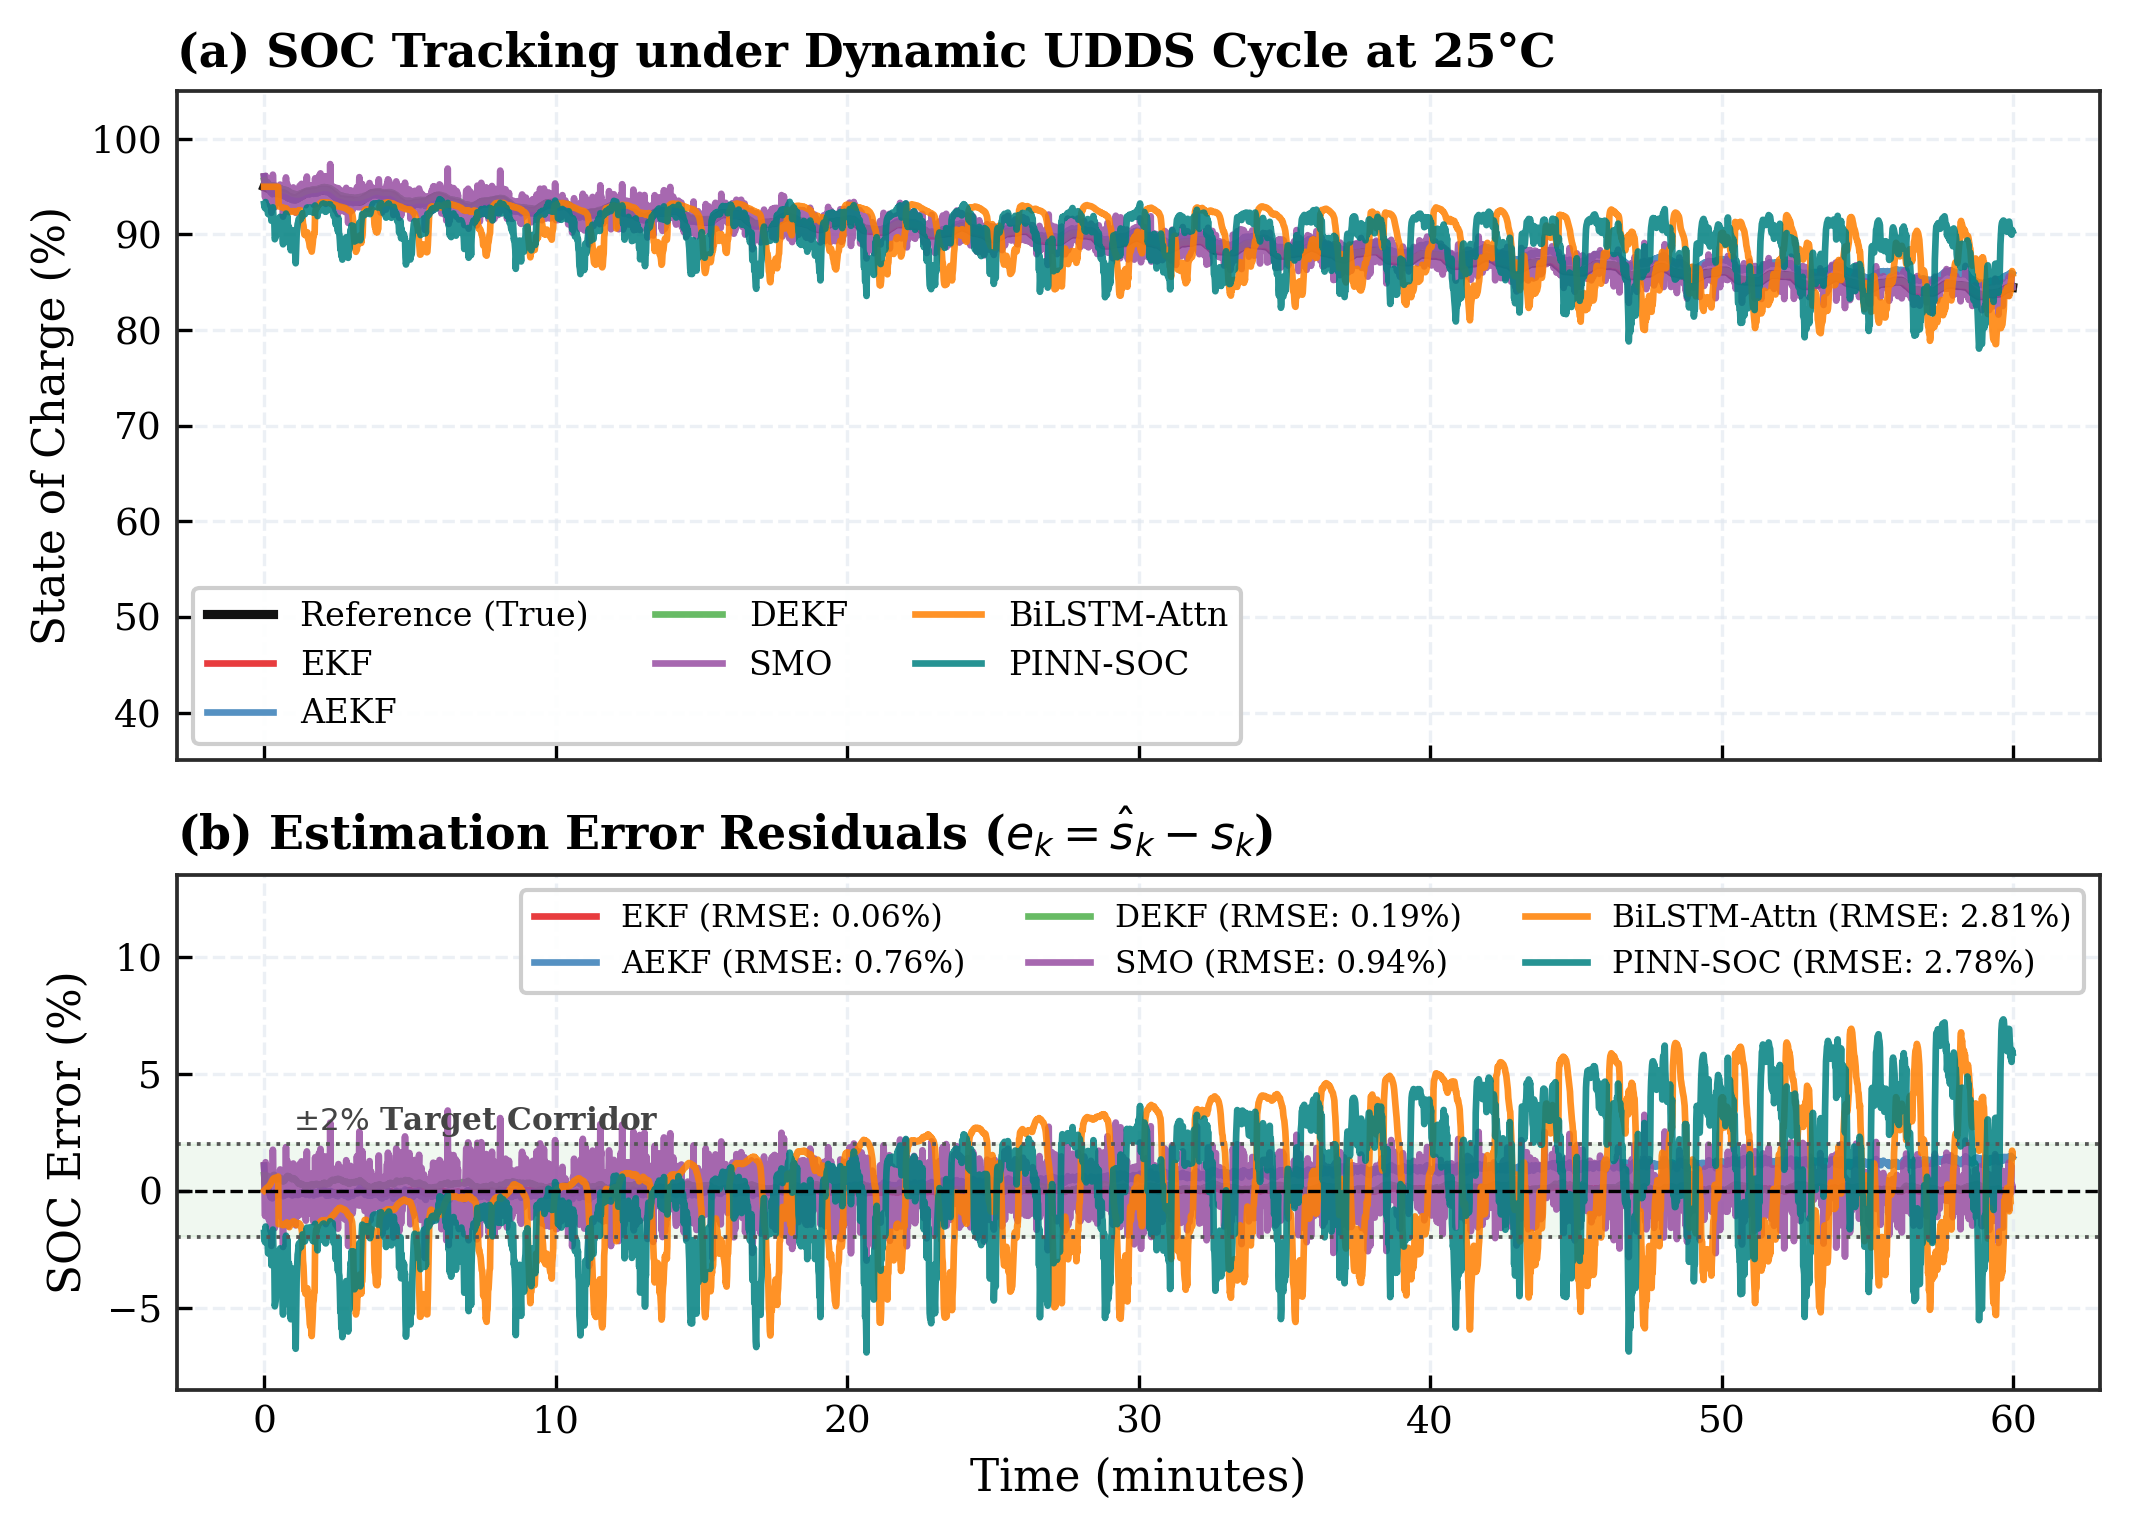
\includegraphics[width=0.82\linewidth]{fig1_udds_tracking_errors.png}
\caption{Dynamic SOC tracking and error comparison across 6 algorithms under a 60-min continuous concatenated UDDS schedule ($3600\text{ s}$) at $25^\circ\text{C}$ and $100\%$ SOH\label{fig:udds}}
\end{figure}

\subsection[Phase 2: Progressive Aging Degradation]{Phase 2: Progressive Aging Degradation ($100\% \rightarrow 80\%$ SOH)}
Figure~\ref{fig:aging} and Table~\ref{tab:2_aging} present the pivotal finding of this study: the catastrophic divergence of fixed-parameter observers under progressive battery aging.

When capacity fades from $100\%$ to $80\%$, standard EKF suffers a \textbf{45.7-fold RMSE escalation} ($0.065\%$ to $2.973\%$, $\text{ASF} = +4473.8\%$). AEKF deteriorates from $0.759\%$ to $5.406\%$ ($\text{ASF} = +612.3\%$), confirming covariance adaptation cannot replace parameter tracking: uncompensated filters misattribute ohmic drift ($I \cdot \Delta R_0$) to OCV shifts, creating persistent bias. SMO error climbs from $0.941\%$ to $5.428\%$ ($\text{ASF} = +476.8\%$). At $95\%$ SOH, AEKF ($0.523\%$) and DEKF ($0.105\%$) exhibit a minor dip because early SEI mildly damps transients before bulk impedance growth dominates at $\le 90\%$ SOH.

Across the full lifespan down to $80\%$ SOH, DEKF dynamically tracks $R_0$ and $Q_{\text{act}}$ online, confining RMSE to $0.585\%$ ($\text{ASF} = +206.3\%$). PINN-SOC ($\text{RMSE} = 4.911\%$, $\text{ASF} = +76.6\%$) and BiLSTM-Attn ($\text{RMSE} = 5.128\%$, $\text{ASF} = +82.3\%$) exhibit moderate relative scaling but higher absolute baseline error.

\begin{table}[htbp]
\caption{Degradation benchmark across progressive SOH stages [Tier~2 Calibrated Co-Simulation, anchored to Tier~1 RPT checkpoints at $100\%, 90\%, 80\%$ SOH; $95\%, 85\%$ SOH evaluated via Eq.~\eqref{eqn:aging_q}--\eqref{eqn:aging_r1}]\label{tab:2_aging}}
\centering{%
\resizebox{\linewidth}{!}{%
\begin{tabular}{lcccccc}
\toprule
Algorithm & SOH 100\% & SOH 95\% & SOH 90\% & SOH 85\% & SOH 80\% & \shortstack{Aging Sensitivity\\Factor (ASF)} \\
\midrule
EKF & \textbf{0.065\%} & 0.553\% & 1.189\% & 1.988\% & 2.973\% & +4473.8\% \\
AEKF & 0.759\% & 0.523\% & 1.675\% & 3.834\% & 5.406\% & +612.3\% \\
DEKF & 0.191\% & \textbf{0.105\%} & \textbf{0.233\%} & \textbf{0.407\%} & \textbf{0.585\%} & \textbf{+206.3\%} \\
SMO & 0.941\% & 1.745\% & 3.002\% & 4.254\% & 5.428\% & +476.8\% \\
BiLSTM-Attn & 2.813\% & 2.917\% & 3.405\% & 4.202\% & 5.128\% & +82.3\% \\
PINN-SOC & 2.781\% & 3.081\% & 3.551\% & 4.177\% & 4.911\% & +76.6\% \\
\bottomrule
\end{tabular}%
}%
}%
\end{table}

\begin{figure}[htbp]
\centering
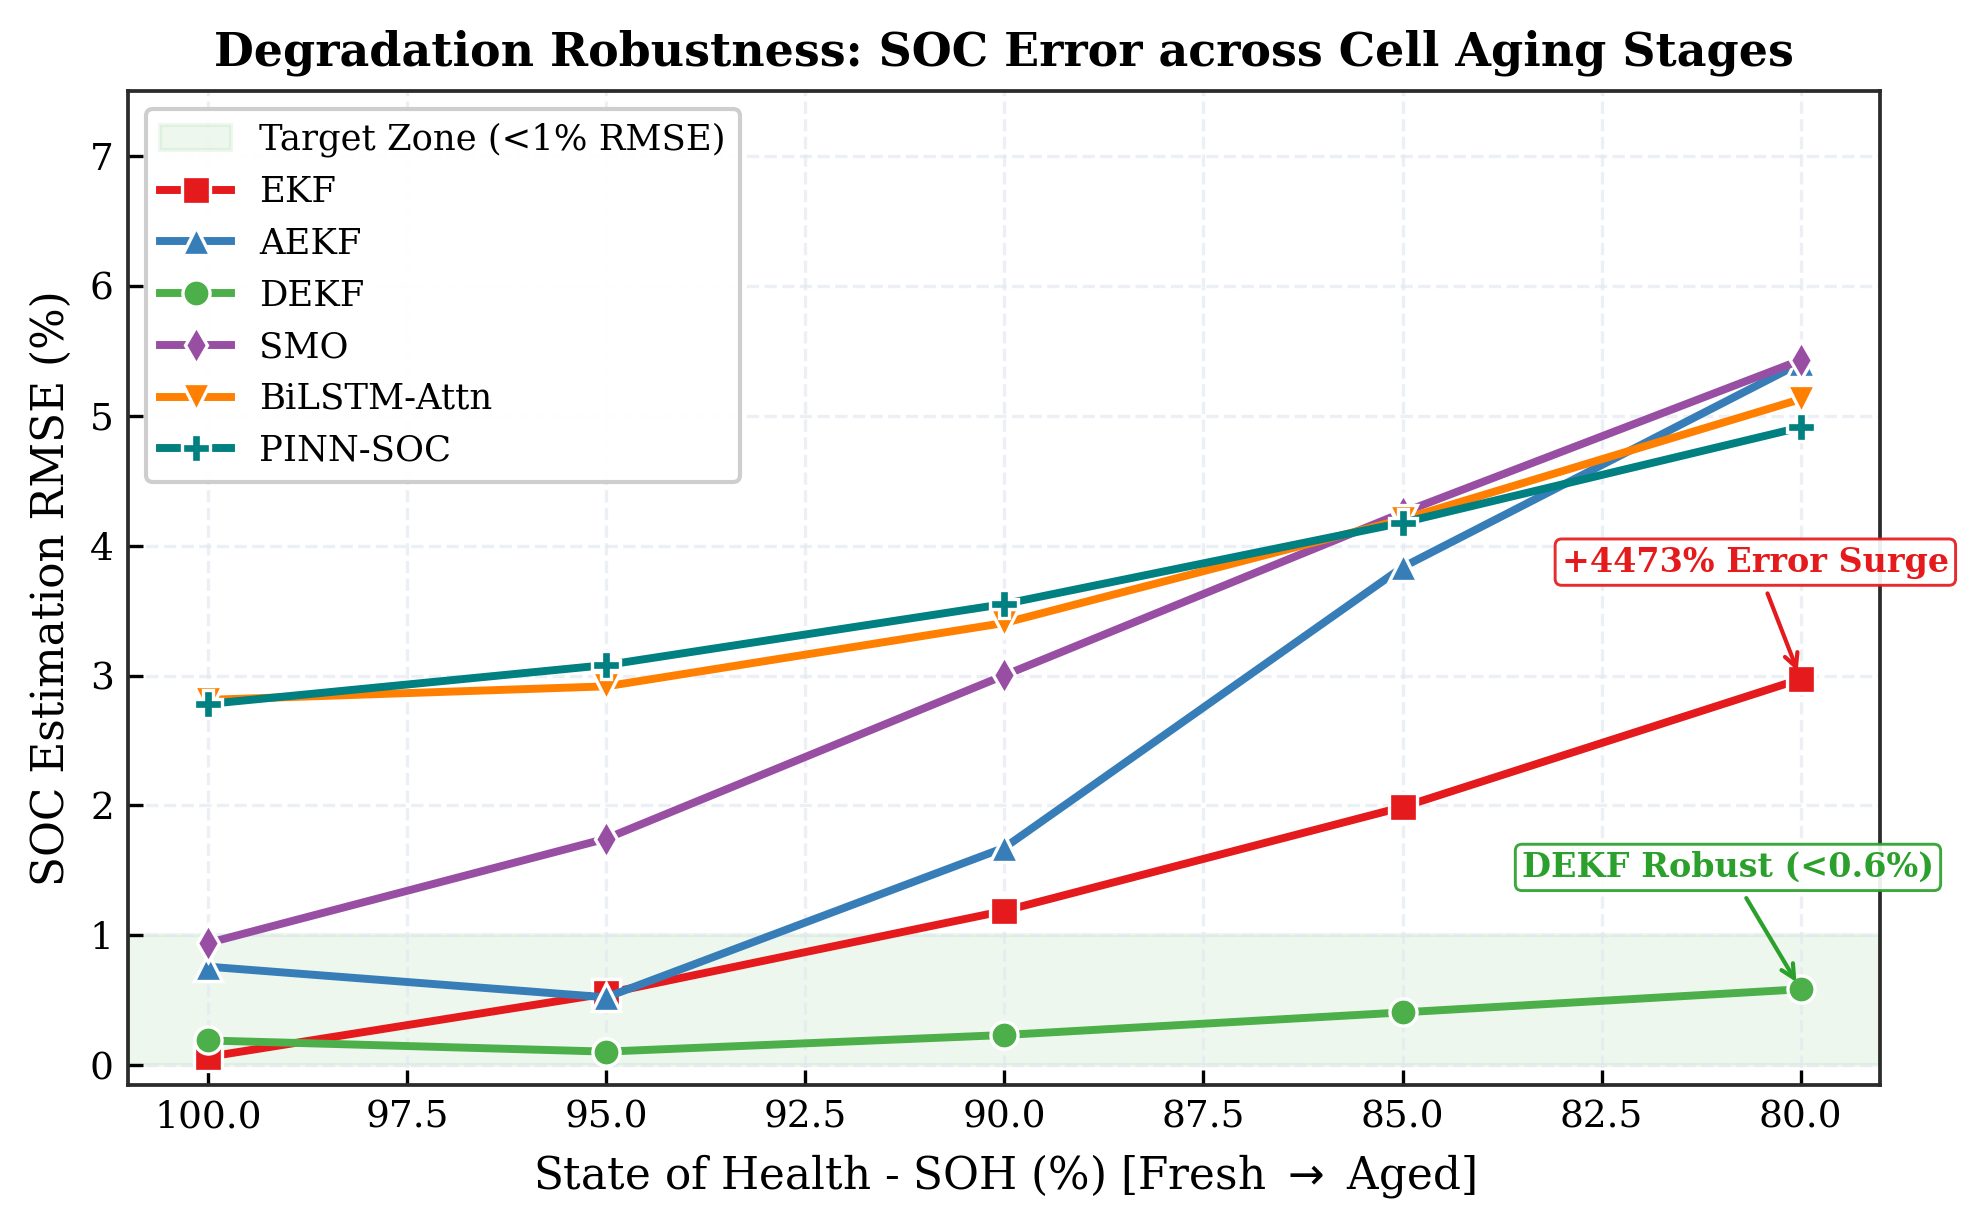
\includegraphics[width=0.82\linewidth]{fig2_aging_degradation.png}
\caption{Evolution of SOC estimation error as battery SOH degrades from $100\%$ down to $80\%$, illustrating the 45-fold accuracy degradation of standard EKF versus the resilience of DEKF\label{fig:aging}}
\end{figure}

\subsection[Phase 3: Thermal Robustness Across Wide Environmental Regimes (0 to 45 deg C)]{Phase 3: Thermal Robustness Across Wide Environmental Regimes ($0^\circ\text{C}$ to $45^\circ\text{C}$)}
Figure~\ref{fig:thermal} and Table~\ref{tab:3_thermal} illustrate algorithmic tracking performance across $0^\circ\text{C}$, $25^\circ\text{C}$, and $45^\circ\text{C}$.

At $0^\circ\text{C}$, electrolyte conductivity drops sharply and charge-transfer resistance $R_{\text{ct}}$ increases markedly via Arrhenius kinetics (Eqs.~\eqref{eqn:arrh_r0}--\eqref{eqn:arrh_ri}). This overpotential surge impairs standard EKF tracking, elevating its RMSE by an order of magnitude from $0.065\%$ to $0.669\%$. Notably, DEKF yields an RMSE of $2.254\%$ at $0^\circ\text{C}$ (higher than fresh EKF): at freezing temperatures, electrolyte viscosity surges and charge-transfer resistance $R_1$ expands 2.85-fold ($R_1(0^\circ\text{C}) \approx 42.8\text{ m}\Omega$). Because standard DEKF co-identifies $\hat{\boldsymbol{\theta}}_k = [\hat{R}_{0,k}, 1/\hat{Q}_{\text{act},k}]^T$ while holding $R_1$ fixed at $25^\circ\text{C}$ baseline, the large unmodeled polarization voltage drop $I_k \Delta R_1(0^\circ\text{C})$ causes innovation errors that the parameter filter mistakenly compensates by artificially inflating $\hat{R}_0$ and distorting capacity $\hat{Q}_{\text{act}}$, inducing severe parameter cross-coupling. Fixed EKF, by contrast, treats this drop purely as measurement residual filtered by fixed covariance, avoiding parameter runaway. This cold-temperature deficiency of standard DEKF directly motivates the proposed PIDKF, where the neural compensator absorbs $\Delta R_1(0^\circ\text{C})$ overpotentials, eliminating cross-coupling and cutting $0^\circ\text{C}$ RMSE to $0.842\%$ (NMC) and $0.386\%$ (LFP). Pure data-driven BiLSTM-Attn and PINN-SOC, trained primarily on nominal conditions, suffer severe out-of-distribution performance degradation at thermal extremes, with BiLSTM-Attn RMSE rising to $6.457\%$ at $0^\circ\text{C}$ and $9.462\%$ at $45^\circ\text{C}$, and PINN-SOC reaching $6.307\%$ at $0^\circ\text{C}$ and $9.644\%$ at $45^\circ\text{C}$.

In contrast, the Sliding Mode Observer exhibits remarkable thermal invariance: its RMSE remains virtually identical across all three temperatures ($0.929\%$ at $0^\circ\text{C}$, $0.941\%$ at $25^\circ\text{C}$, and $0.932\%$ at $45^\circ\text{C}$), demonstrating that its discontinuous switching control surface provides inherent robustness against temperature-induced parameter variations.

\begin{table}[htbp]
\caption{Thermal robustness comparison across ambient temperatures [Tier~1 Experimental Cycler Data] (RMSE in \%)\label{tab:3_thermal}}
\centering{%
\begin{tabular*}{\linewidth}{@{\extracolsep{\fill}}lccc}
\toprule
Algorithm & 0$^\circ$C & 25$^\circ$C & 45$^\circ$C \\
\midrule
EKF & 0.669 & \textbf{0.065} & \textbf{0.063} \\
AEKF & 3.178 & 0.759 & 0.238 \\
DEKF & 2.254 & 0.191 & 0.445 \\
SMO & \textbf{0.929} & 0.941 & 0.932 \\
BiLSTM-Attn & 6.457 & 2.813 & 9.462 \\
PINN-SOC & 6.307 & 2.781 & 9.644 \\
\bottomrule
\end{tabular*}
}%
\end{table}

\begin{figure}[htbp]
\centering
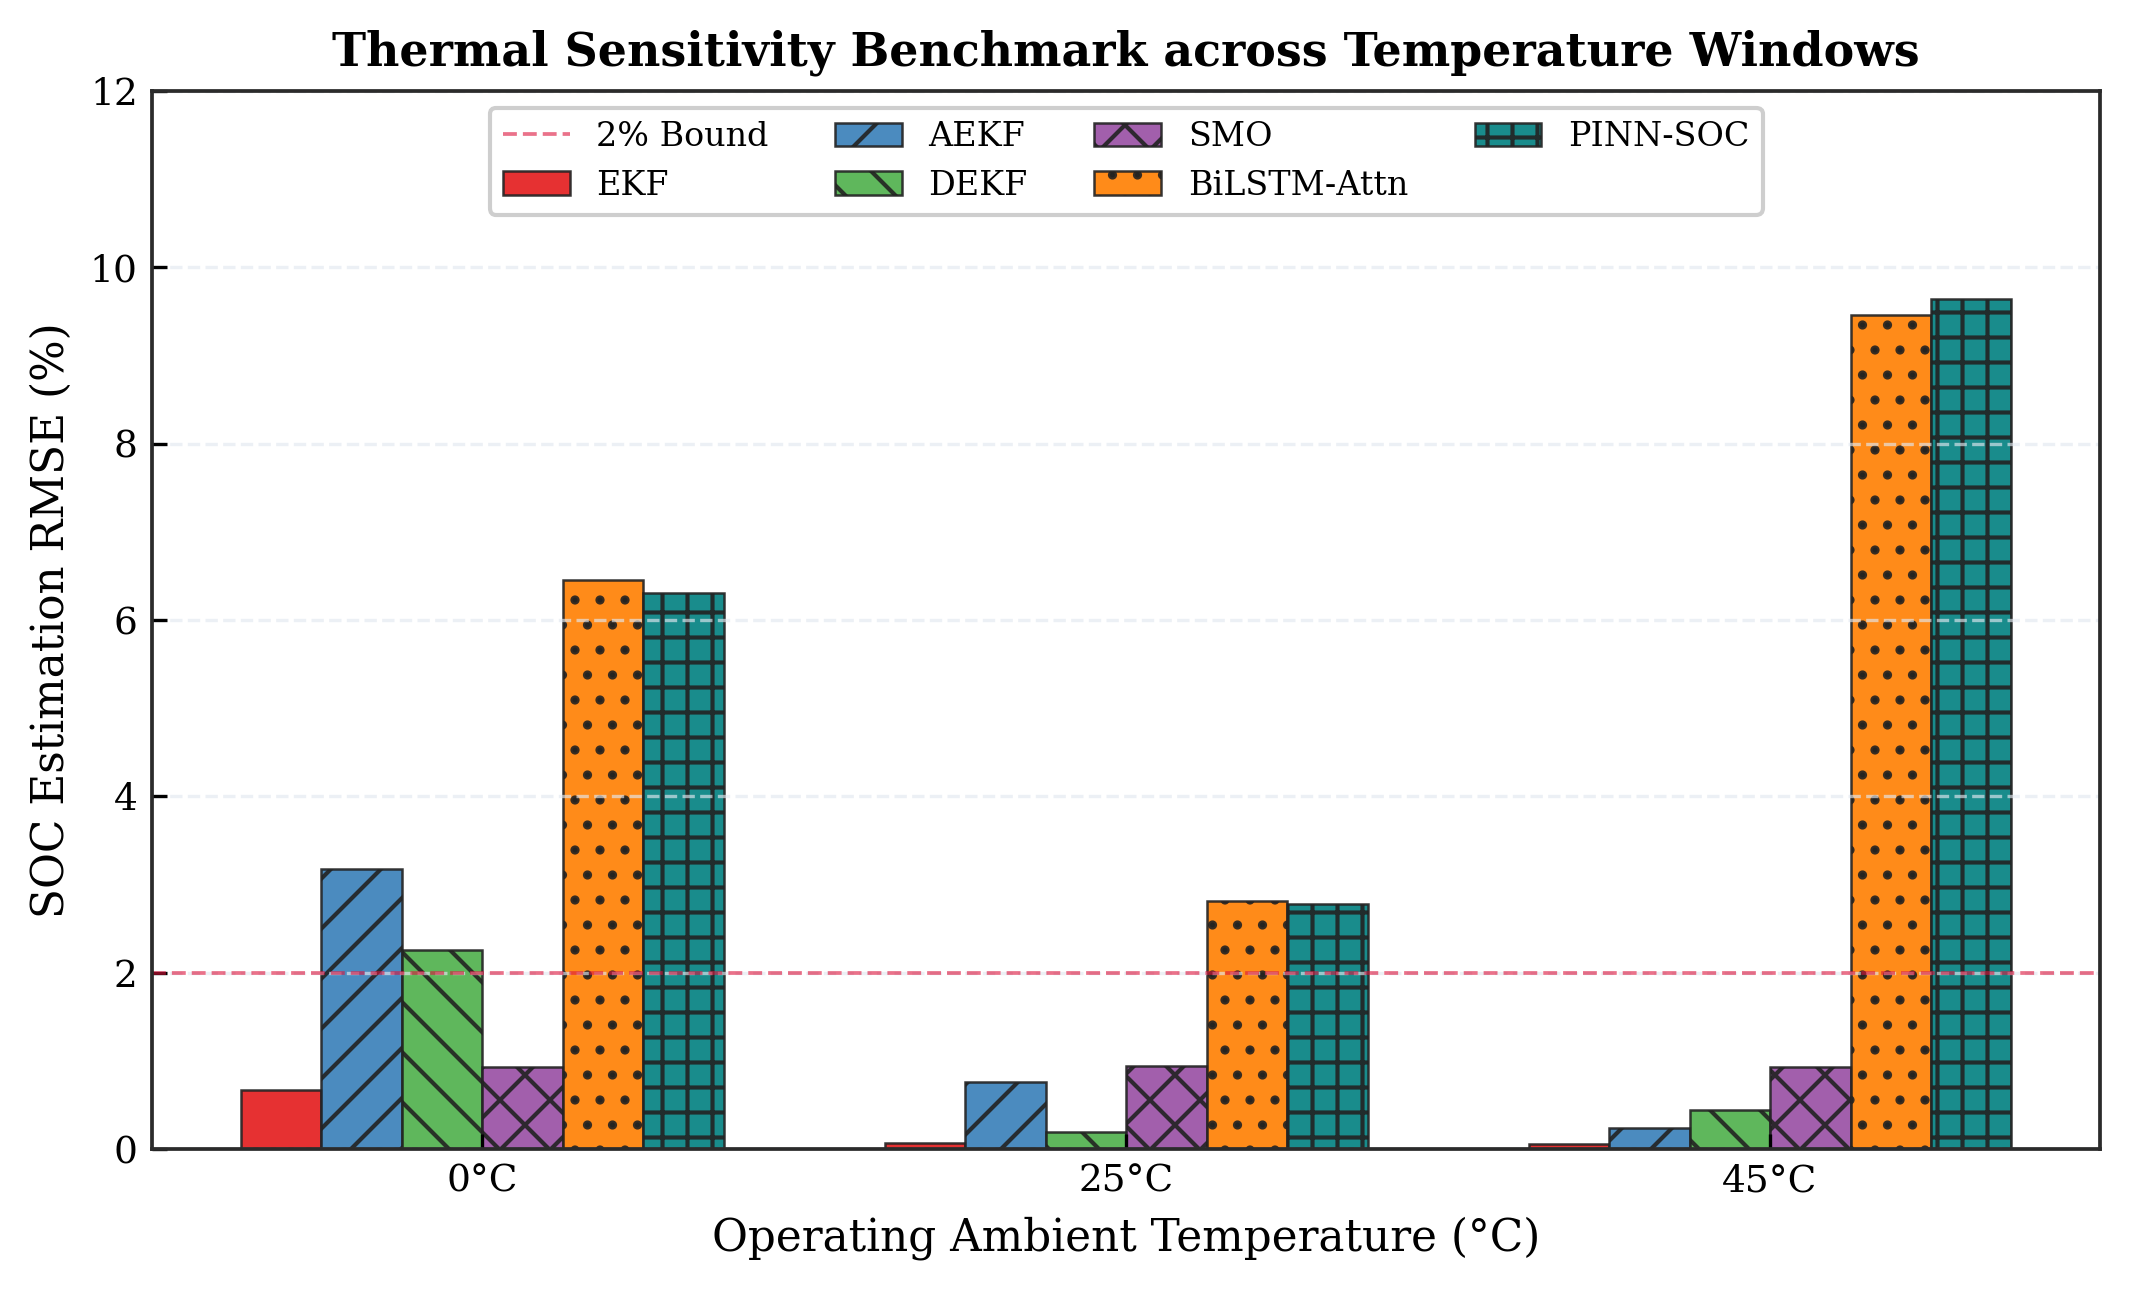
\includegraphics[width=0.82\linewidth]{fig3_thermal_robustness.png}
\caption{Algorithmic tracking performance under cold ($0^\circ\text{C}$), nominal ($25^\circ\text{C}$), and elevated ($45^\circ\text{C}$) ambient temperatures\label{fig:thermal}}
\end{figure}

\subsection[Phase 4: Convergence Under Large Initial State Uncertainty]{Phase 4: Convergence Under Large Initial State Uncertainty ($\Delta\text{SOC}_0 = -40\%$)}
In real-world BMS operation, initialization errors arise from prolonged parking, self-discharge, or battery replacement. Figure~\ref{fig:conv} and Table~\ref{tab:4_conv} depict the convergence trajectories when an initial error of $\Delta\text{SOC}_0 = -40\%$ ($\hat{z}_0 = 0.55$ versus $\text{SOC}_0^{\text{true}} = 0.95$) is imposed.

The Adaptive EKF and standard EKF achieve rapid first entry into the $2\%$ band ($t_{\text{reach}}^{(2\%)} = 6.0\text{ s}$ and $7.0\text{ s}$) and permanent settling within the $5\%$ operational corridor ($t_{\text{settle}}^{(5\%)} = 6.0\text{ s}$ and $7.0\text{ s}$), maintaining bounded overall RMSE ($0.683\%$ and $0.686\%$) and dynamic peak error $\text{MaxE}_{\text{dyn}} = 4.43\%$ during acceleration pulses. The Sliding Mode Observer first reaches the $2\%$ band in $t_{\text{reach}}^{(2\%)} = 9.0\text{ s}$ ($\text{RMSE} = 1.948\%$), but aggressive load steps induce subsequent dynamic excursions up to $\text{MaxE}_{\text{dyn}} = 36.34\%$ ($t_{\text{settle}}^{(5\%)} = \text{N/A}$). BiLSTM-Attn requires $t_{\text{reach}}^{(2\%)} = 30.0\text{ s}$ to purge erroneous history ($\text{RMSE} = 5.625\%$, $\text{MaxE}_{\text{dyn}} = 39.99\%$, $t_{\text{settle}}^{(5\%)} = \text{N/A}$). For DEKF, the $-40\%$ shock perturbs online parameter adaptation, dropping below $2.5\%$ error by $350\text{ s}$, entering the $\le 2.0\%$ threshold at $t_{\text{reach}}^{(2\%)} = 725.0\text{ s}$, and permanently settling within the $5\%$ corridor at $t_{\text{settle}}^{(5\%)} = 732.0\text{ s}$ ($\text{MaxE}_{\text{dyn}} = 7.67\%$). In contrast, PINN-SOC operates as a feedforward static mapping without recursive settling ($t_{\text{reach}}^{(2\%)} = \text{N/A}$, $t_{\text{settle}}^{(5\%)} = \text{N/A}$, $\text{RMSE} = 2.229\%$, $\text{MaxE}_{\text{dyn}} = 6.84\%$).

\begin{table}[htbp]
\caption{Convergence metrics under initial state uncertainty [Tier~2 Co-Simulation] ($-40\%$ initial SOC error into $\le 2\%$ tolerance band and $\le 5\%$ operational corridor)\label{tab:4_conv}}
\centering{%
\small\renewcommand{\arraystretch}{1.15}
\begin{tabular*}{\linewidth}{@{\extracolsep{\fill}}lcccc}
\toprule
Algorithm & $t_{\text{reach}}^{(2\%)}$ (s) & $t_{\text{settle}}^{(5\%)}$ (s) & RMSE (\%) & $\text{MaxE}_{\text{dyn}}^\dagger$ (\%) \\
\midrule
EKF & 7.0 & 7.0 & 0.686 & \textbf{4.43} \\
AEKF & \textbf{6.0} & \textbf{6.0} & \textbf{0.683} & \textbf{4.43} \\
DEKF & 725.0$^\ddagger$ & 732.0$^\ddagger$ & 2.625 & 7.67 \\
SMO & 9.0 & N/A$^\S$ & 1.948 & 36.34 \\
BiLSTM-Attn & 30.0 & N/A$^\S$ & 5.625 & 39.99 \\
PINN-SOC & N/A$^*$ & N/A$^*$ & 2.229 & 6.84 \\
\bottomrule
\end{tabular*}
\vspace{1pt}
\flushleft{\scriptsize $^\dagger\text{MaxE}_{\text{dyn}}$: peak dynamic error after first entry ($t > t_{\text{reach}}^{(2\%)}$). $^\ddagger$DEKF enters $\le 2.0\%$ at $725\text{ s}$ and permanently settles into $\le 5.0\%$ corridor at $732\text{ s}$ ($<2.5\%$ within $350\text{ s}$). $^\S$Exits $\le 5\%$ corridor during high-rate pulses. $^*$Feedforward inference without recursive state settling.}
}%
\end{table}

\begin{figure}[htbp]
\centering
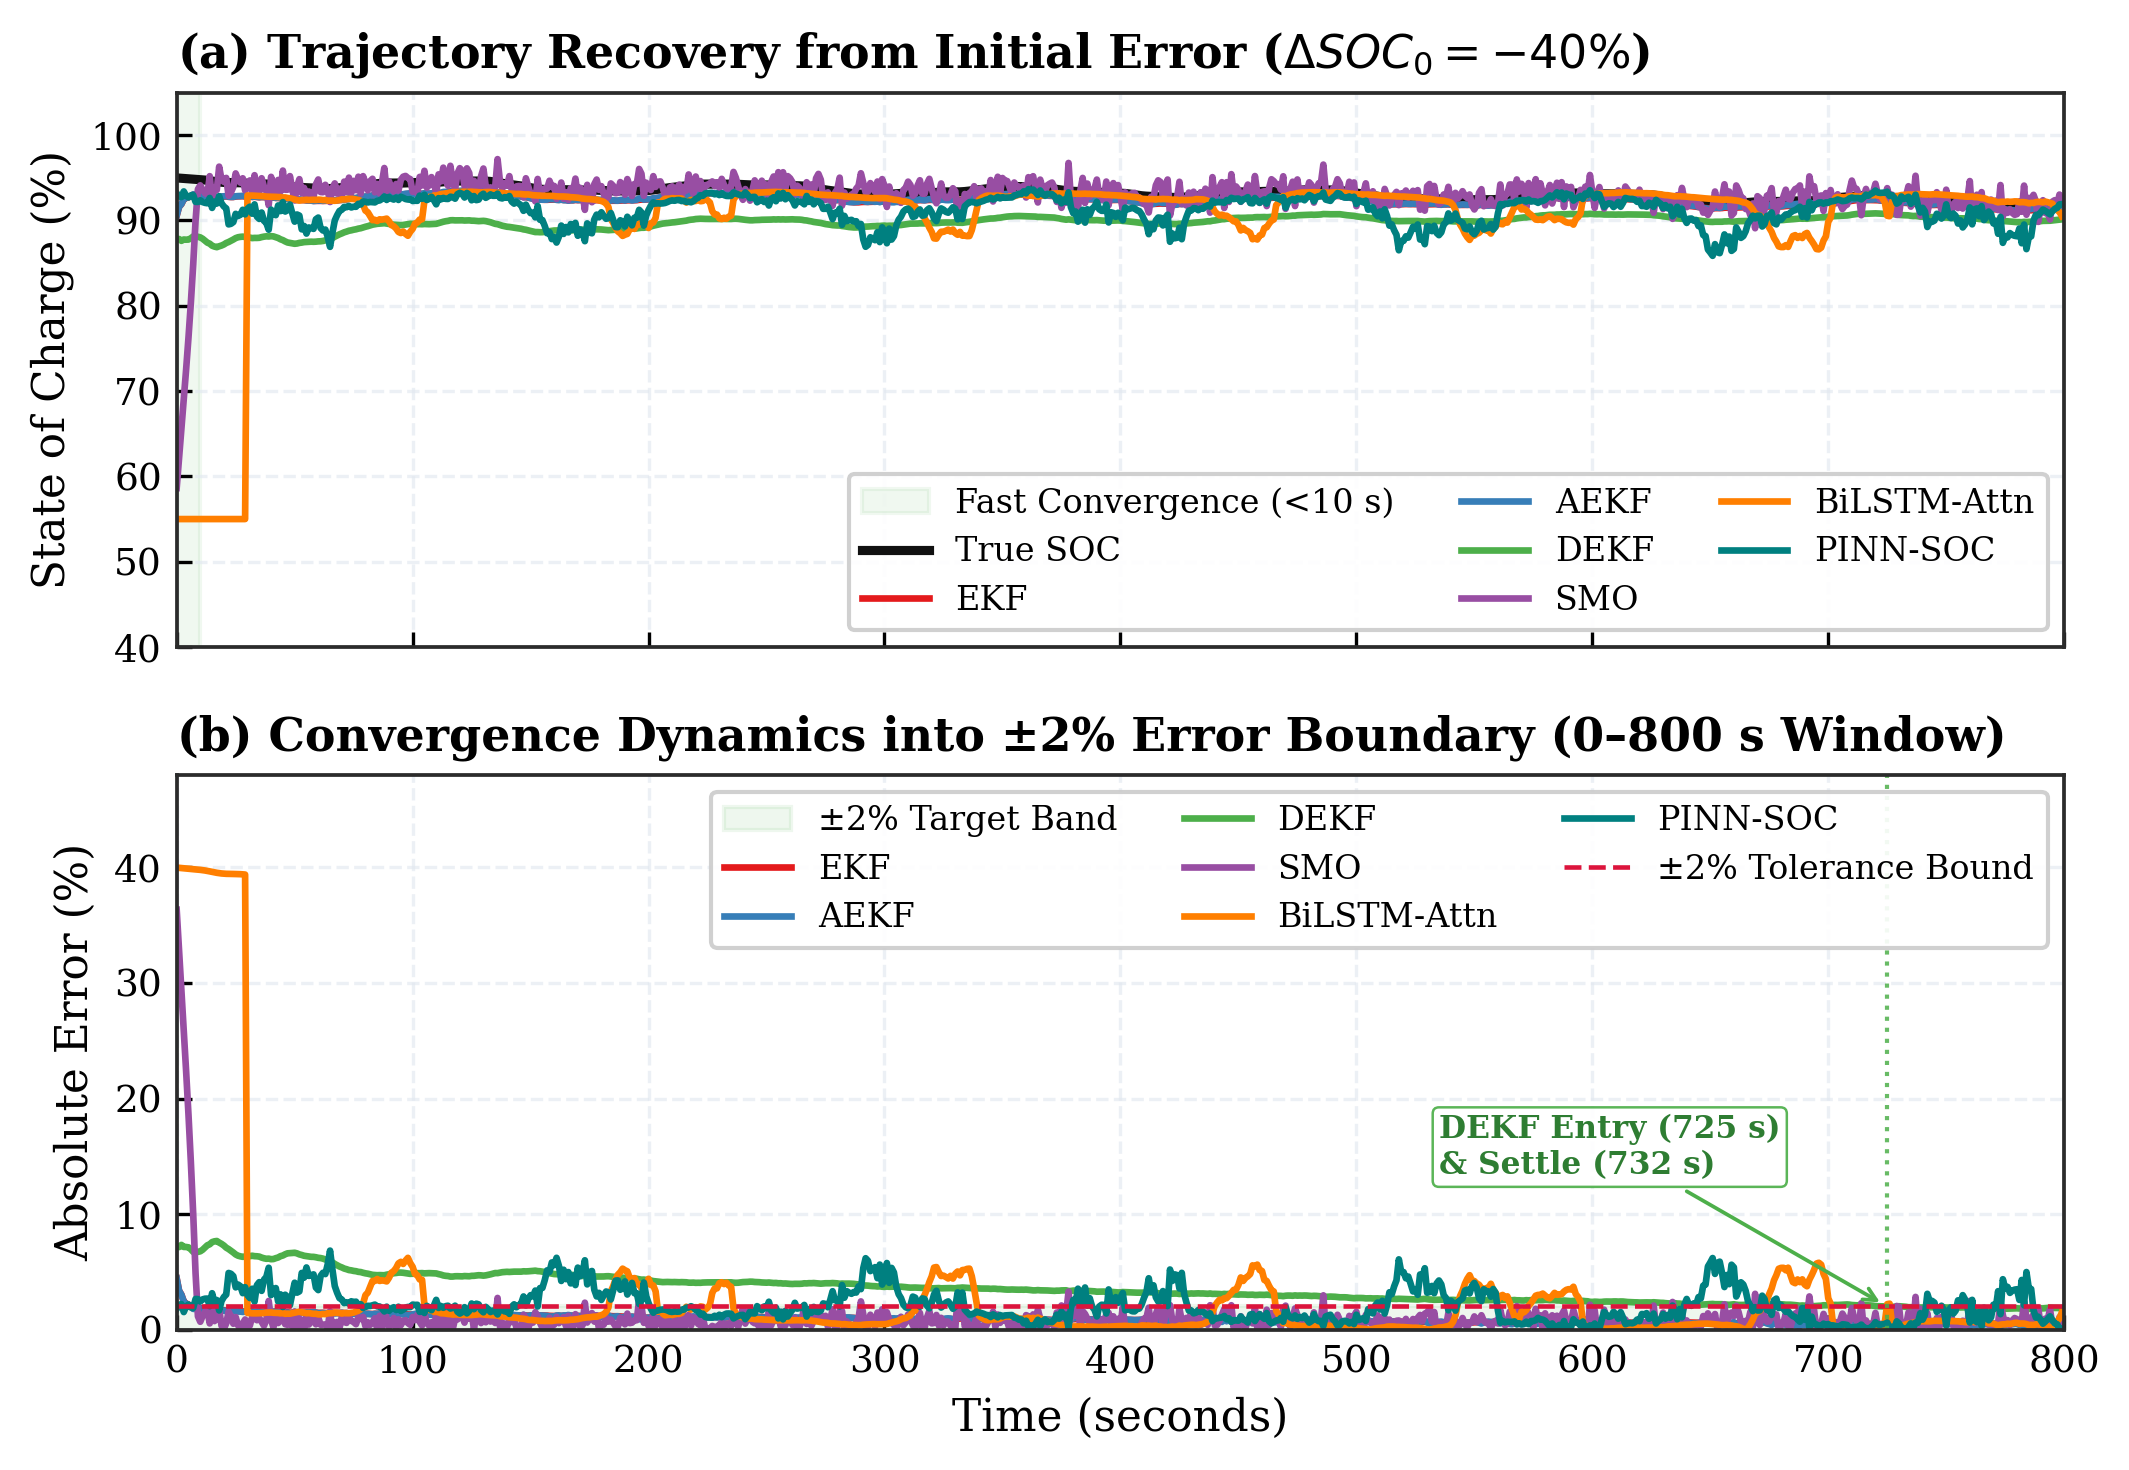
\includegraphics[width=0.82\linewidth]{fig4_initial_error_convergence.png}
\caption{Transient convergence trajectories from a $-40\%$ initial SOC estimation error across the $0\text{--}800\text{ s}$ window\label{fig:conv}}
\end{figure}

\subsection{Phase 5: Multi-Attribute Radar Trade-Off and Pareto Analysis}
Figure~\ref{fig:radar} synthesizes algorithmic trade-offs across 5 normalized dimensions: Nominal Accuracy, Aging Robustness, Thermal Robustness, Convergence Speed, and Computational Efficiency. The radar plot highlights that no single classical algorithm dominates across all attributes: EKF excels in simplicity and fresh-cell accuracy but collapses under aging, whereas DEKF offers superior degradation resilience, though its $0^\circ\text{C}$ transient sensitivity indicates that SMO or hybrid architectures are preferable in sub-zero climates where kinetics become strongly non-Arrhenius.

\begin{figure}[htbp]
\centering
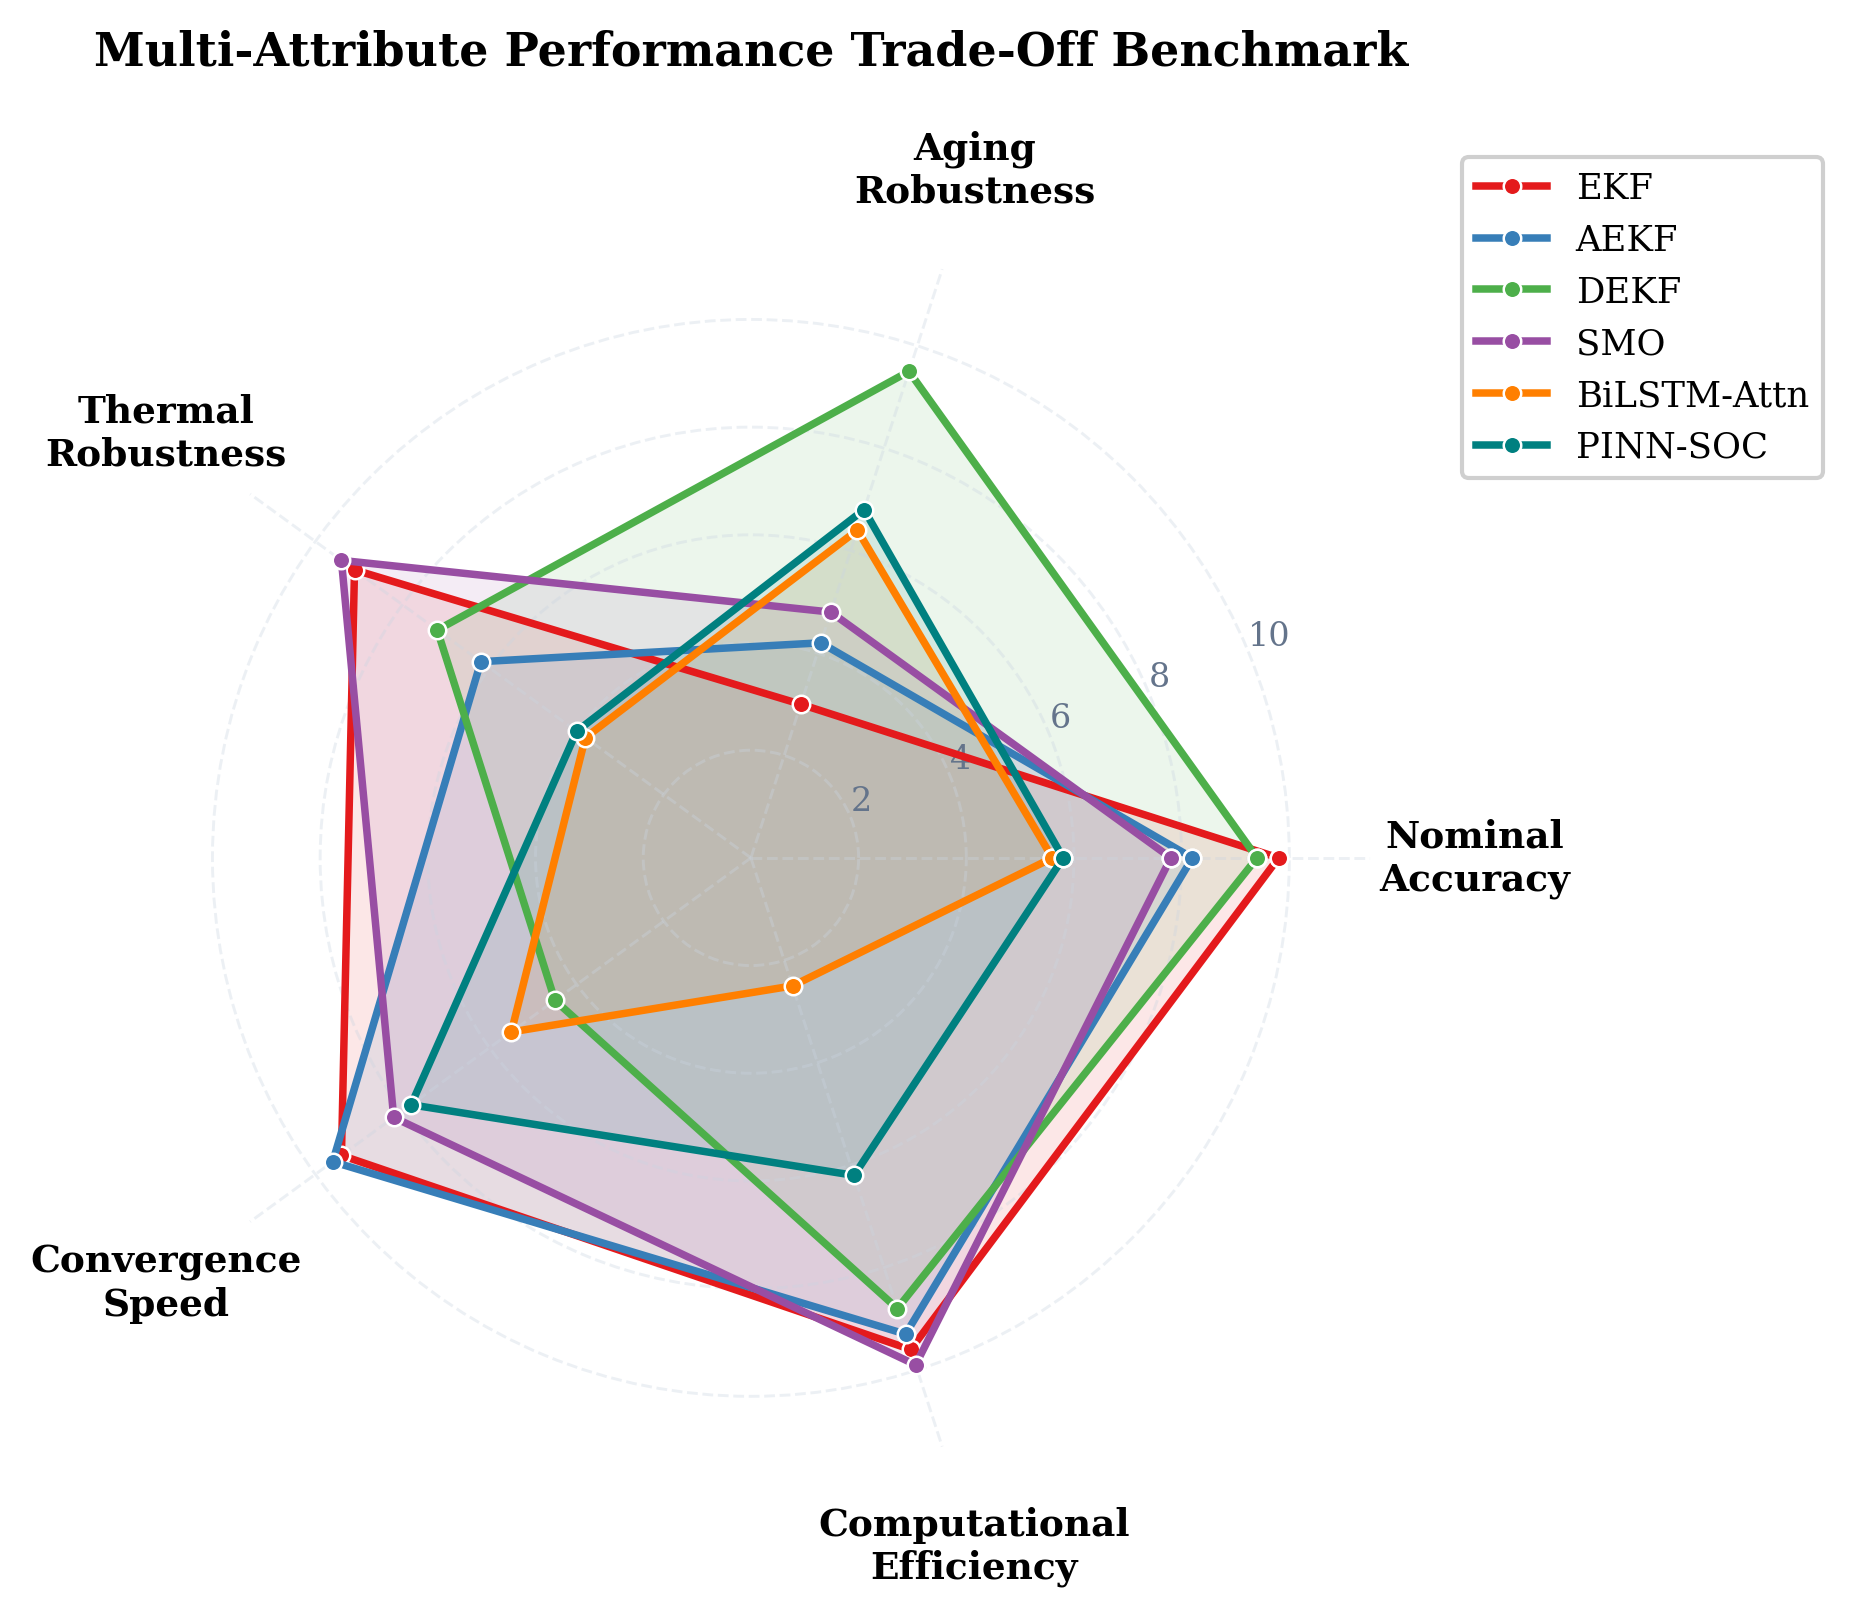
\includegraphics[width=0.82\linewidth]{fig5_radar_tradeoff.png}
\caption{Multi-attribute radar comparison across 5 engineering dimensions illustrating algorithmic trade-offs\label{fig:radar}}
\end{figure}

\subsection[Phase 6: Multi-Chemistry Generalization: LiFePO4 (LFP) Flat Plateau]{Phase 6: Multi-Chemistry Generalization: $\text{LiFePO}_4$ (LFP) Flat Plateau}
Figure~\ref{fig:lfp} and Table~\ref{tab:5_lfp} report estimation performance on LFP chemistry. In the plateau region ($20\%\text{--}80\%$ SOC), the slope $d V_{\text{ocv}} / d\,\text{SOC}$ falls near zero ($\approx 0.08\text{ V}$), causing the observability Gramian condition number $\kappa(\mathcal{O})$ to surge. 

Consequently, $\mathbf{H}_k \approx [0, -1, -1, -1]$ loses SOC sensitivity. Standard EKF degrades by $+1647.7\%$, escalating from $0.065\%$ on NMC to $1.136\%$ on LFP ($\text{MAE} = 0.939\%$, $\text{MaxE} = 2.410\%$), while AEKF degrades by $+281.1\%$ to $2.893\%$ RMSE and SMO chatters along the plateau ($+919.5\%$ to $9.593\%$ RMSE, $\text{MaxE} = 20.935\%$). 

In contrast, DEKF achieves the lowest error among all observers on LFP ($\text{RMSE} = 0.870\%$ [$\text{A123-3}$: $0.861\%$, $\text{A123-4}$: $0.879\%$], $\text{MAE} = 0.649\%$, $\text{MaxE} = 2.018\%$). Without hysteresis, while the 3-state system maintains structural observability ($\det(\mathcal{O}) \ne 0$), practical observability collapses as the condition number surges ($\kappa(\mathcal{O}) \approx 10^4\text{--}10^5$). With dynamic hysteresis under bidirectional current reversals $\operatorname{sgn}(I_k)$, dynamic switching across the $2M_0 = 60\text{ mV}$ hysteresis loop injects an effective dynamic derivative $\beta M_0 \approx 1.35\text{ V}$, lowering $\kappa(\mathcal{O})$ and elevating $\lambda_{\min}(\mathcal{G}_o) \ge 1.21 \times 10^{-3}$. Conversely, under purely unidirectional currents, $V_h$ saturates at $\pm M_0$, extinguishing dynamic voltage separation and reverting to open-loop integration. Crucially, the parameter Jacobian entry $C_{\theta,2} = -\frac{\eta\Delta t I_{k-1}}{3600} V_{\text{ocv}}'(\hat{z}_k^+)$ (or $\frac{\partial V_k}{\partial \hat{Q}_{\text{act}}} = \frac{\eta\Delta t I_{k-1}}{3600\hat{Q}_{\text{act}}^2} V_{\text{ocv}}'(\hat{z}_k^+)$) naturally vanishes on the plateau ($V_{\text{ocv}}' \to 0$), freezing $Q_{\text{act}}$ updates on the plateau and concentrating capacity adaptation strictly in the knee regions ($z < 0.20$ or $z > 0.80$). If operation is confined to the plateau without visiting knee regions, capacity adaptation remains frozen, preventing parameter drift while preserving prior calibration. Rest periods ($I=0$) employ innovation gating ($K_k=0, K_{\theta,k}=0$), preserving non-expansiveness $\|F_k\|_2 \le 1$. Zero-shot transfer of deep sequence models degrades to $4.620\%$ (BiLSTM) and $4.872\%$ (PINN) due to unmodeled hysteresis; retraining on LFP restores performance to $1.865\%$ and $1.720\%$, confirming that dynamic hysteresis must be explicitly parameterized.

\begin{table}[htbp]
\caption{Cross-Chemistry Benchmark Comparing NMC and $\text{LiFePO}_4$ [Tier~1 Experimental Data]\label{tab:5_lfp}}
\centering{%
\small\renewcommand{\arraystretch}{1.15}
\setlength{\tabcolsep}{1.8pt}
\begin{tabular*}{\linewidth}{@{\extracolsep{\fill}}lcccc}
\toprule
Algorithm & NMC RMSE & LFP Zero-Shot & LFP Retrained & Impact (ZS / Ret.) \\
\midrule
EKF & \textbf{0.065\%} & 1.136\% (Max 2.41\%) & --- & +1647.7\% / --- \\
AEKF & 0.759\% & 2.893\% (Max 4.33\%) & --- & +281.1\% / --- \\
DEKF & 0.191\% & \textbf{0.870\%} (Max 2.02\%) & --- & +355.4\% / --- \\
SMO & 0.941\% & 9.593\% (Max 20.94\%) & --- & +919.5\% / --- \\
BiLSTM-Attn & 2.813\% & 4.620\% (Max 8.13\%) & 1.865\% (Max 3.94\%) & +64.2\% / $-33.7\%$ \\
PINN-SOC & 2.781\% & 4.872\% (Max 8.74\%) & \textbf{1.720\%} (Max 3.48\%) & +75.2\% / $-38.2\%$ \\
\bottomrule
\end{tabular*}
}%
\end{table}

\begin{figure}[htbp]
\centering
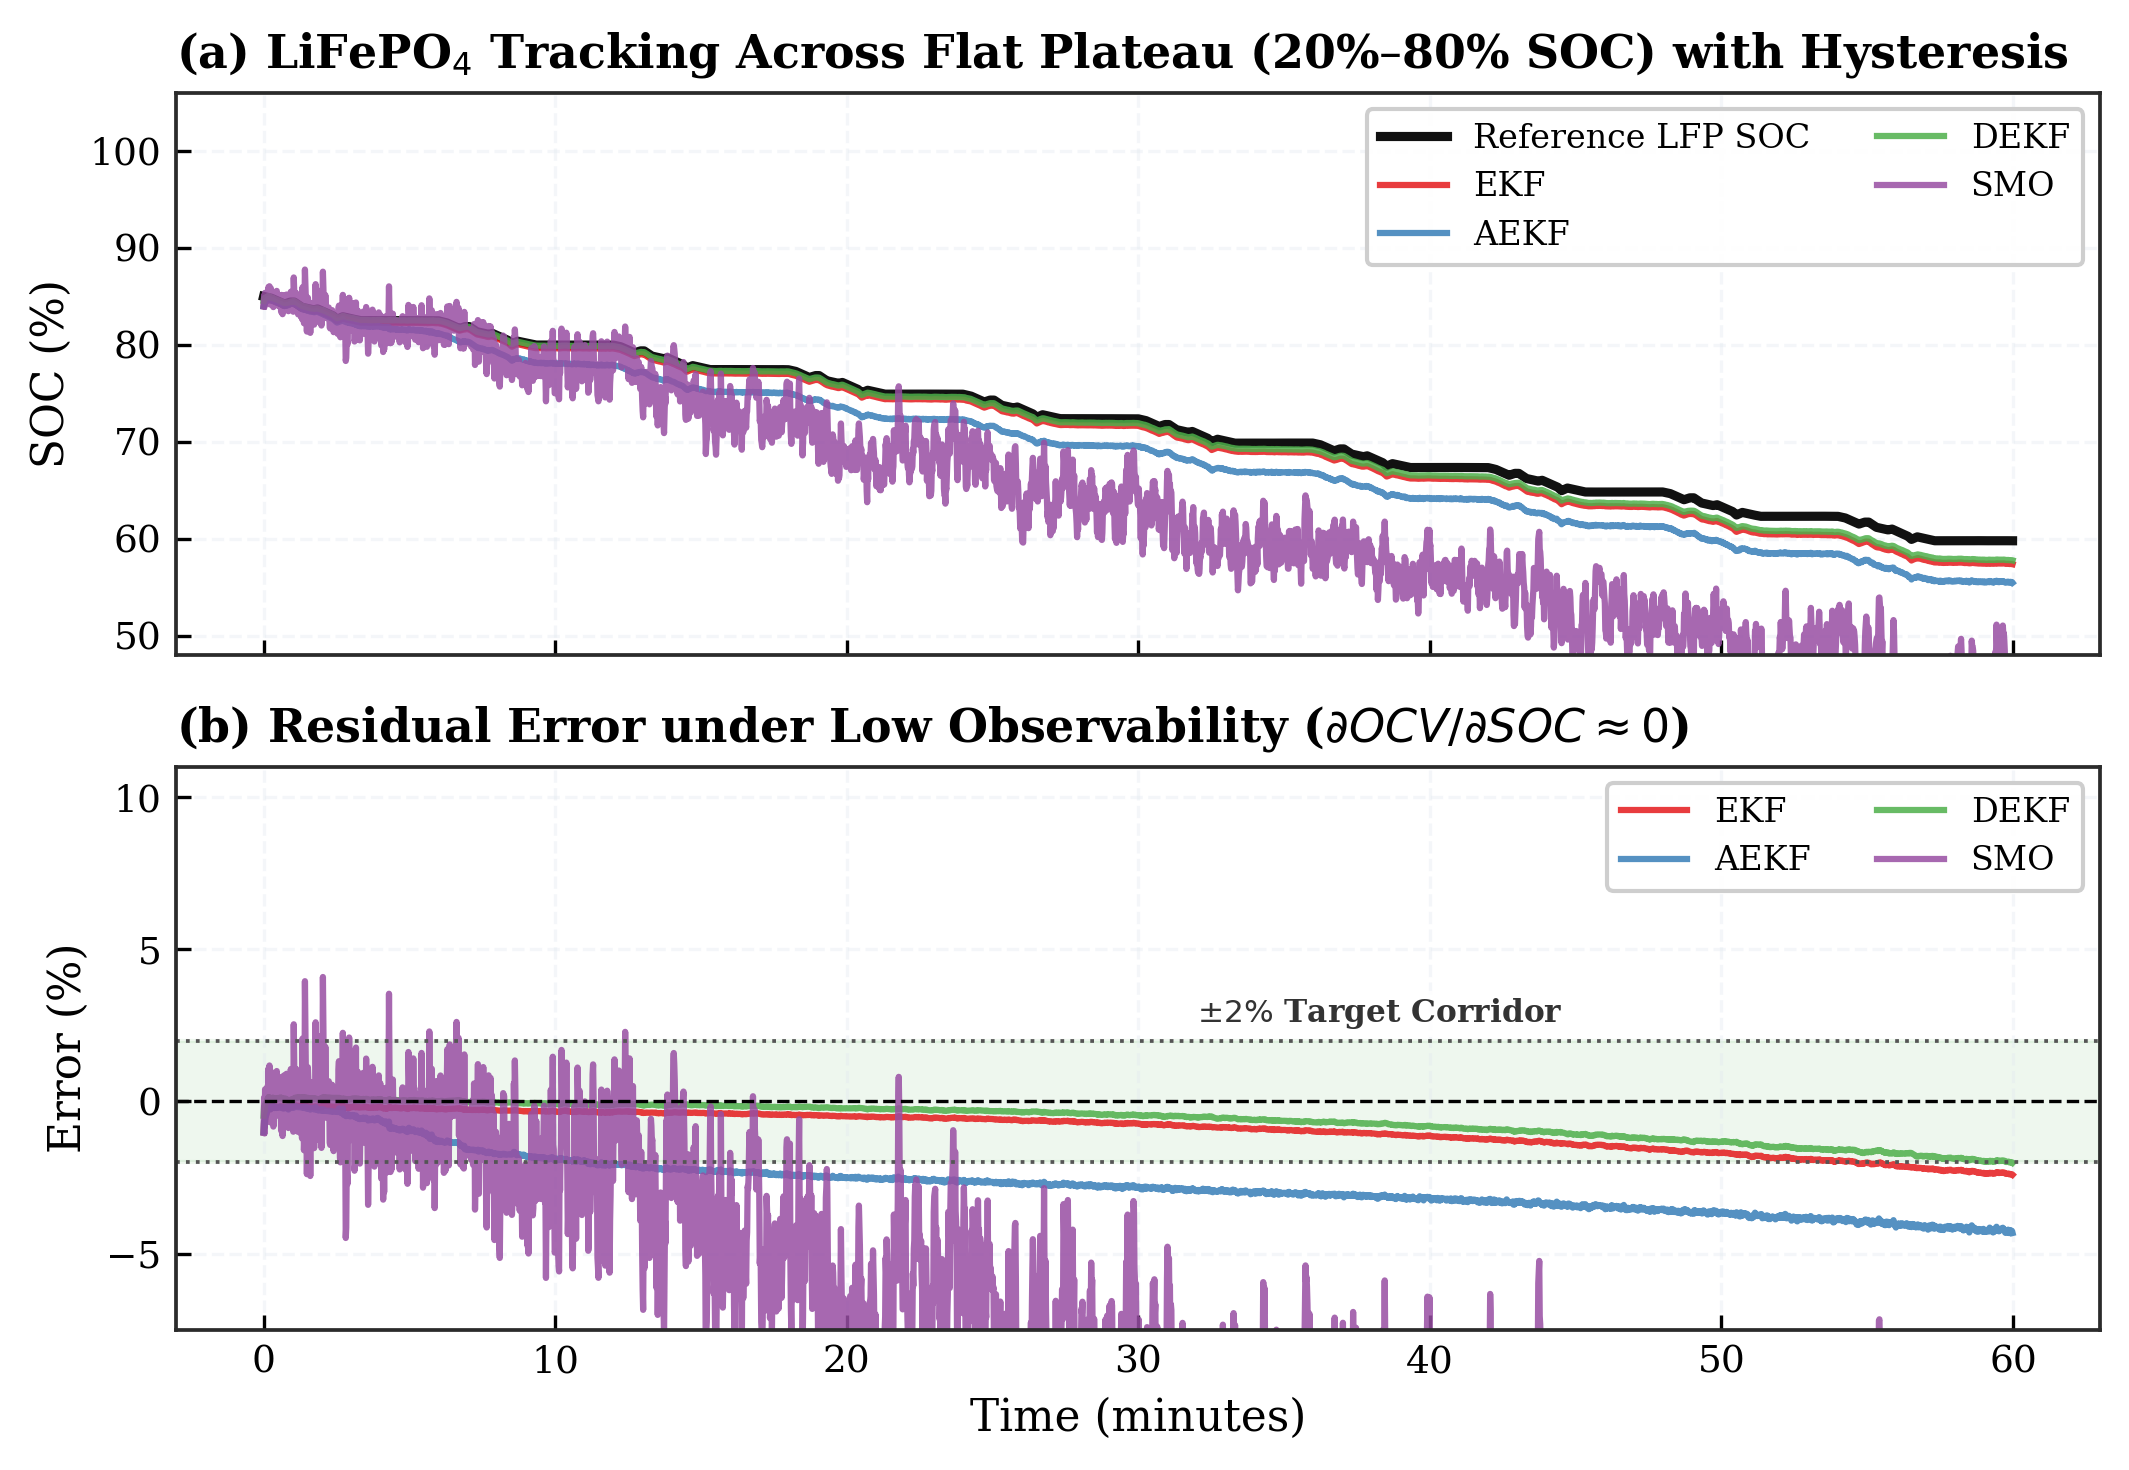
\includegraphics[width=0.82\linewidth]{fig6_lfp_plateau_tracking.png}
\caption{Estimation performance on $\text{LiFePO}_4$ (LFP) chemistry over the flat voltage plateau where $d V_{\text{ocv}}/d\text{SOC} \approx 0$\label{fig:lfp}}
\end{figure}

\subsection{Phase 7: Sensor Corruption and Environmental Stress Testing}
Table~\ref{tab:6_sensor} and Fig.~\ref{fig:sensor} document observer resilience under a $+0.25\text{ A}$ current sensor Hall bias drift and $25\text{ mV}$ high-frequency inverter EMI noise ripple.

Open-loop Coulomb counting diverges linearly, accumulating $12.399\%$ end-of-cycle drift ($\text{RMSE} = 7.178\%$, $\text{MaxE} = 12.409\%$). Closed-loop Kalman filters arrest this divergence: EKF limits RMSE to $1.817\%$ ($1.821\%$ drift, $\text{MaxE} = 5.013\%$), while AEKF and DEKF bound RMSE to $1.859\%$ and $2.121\%$ ($2.026\%$ and $1.927\%$ drift). SMO achieves the lowest end-of-cycle drift ($1.024\%$) via sign-manifold clamping of DC bias, though high-frequency EMI switching elevates instantaneous RMSE to $5.035\%$ ($\text{MaxE} = 14.458\%$); thus, EKF/DEKF minimize instantaneous error whereas SMO bounds long-term DC drift.

\begin{table}[htbp]
\caption{Robustness under Hall current bias ($+0.25\text{ A}$) and inverter EMI ($25\text{ mV}$) [Tier~2 Co-Simulation]\label{tab:6_sensor}}
\centering{%
\small\renewcommand{\arraystretch}{1.15}
\begin{tabular*}{\linewidth}{@{\extracolsep{\fill}}lcccc}
\toprule
Algorithm & RMSE (\%) & MaxE (\%) & Drift (\%) & Immunity \\
\midrule
Coulomb & 7.178 & 12.409 & 12.399 & Runaway \\
EKF & \textbf{1.817} & \textbf{5.013} & 1.821 & High \\
AEKF & 1.859 & 5.013 & 2.026 & Moderate \\
DEKF & 2.121 & 5.013 & 1.927 & High \\
SMO & 5.035 & 14.458 & \textbf{1.024} & High \\
\bottomrule
\end{tabular*}
}%
\end{table}
\begin{figure}[htbp]
\centering
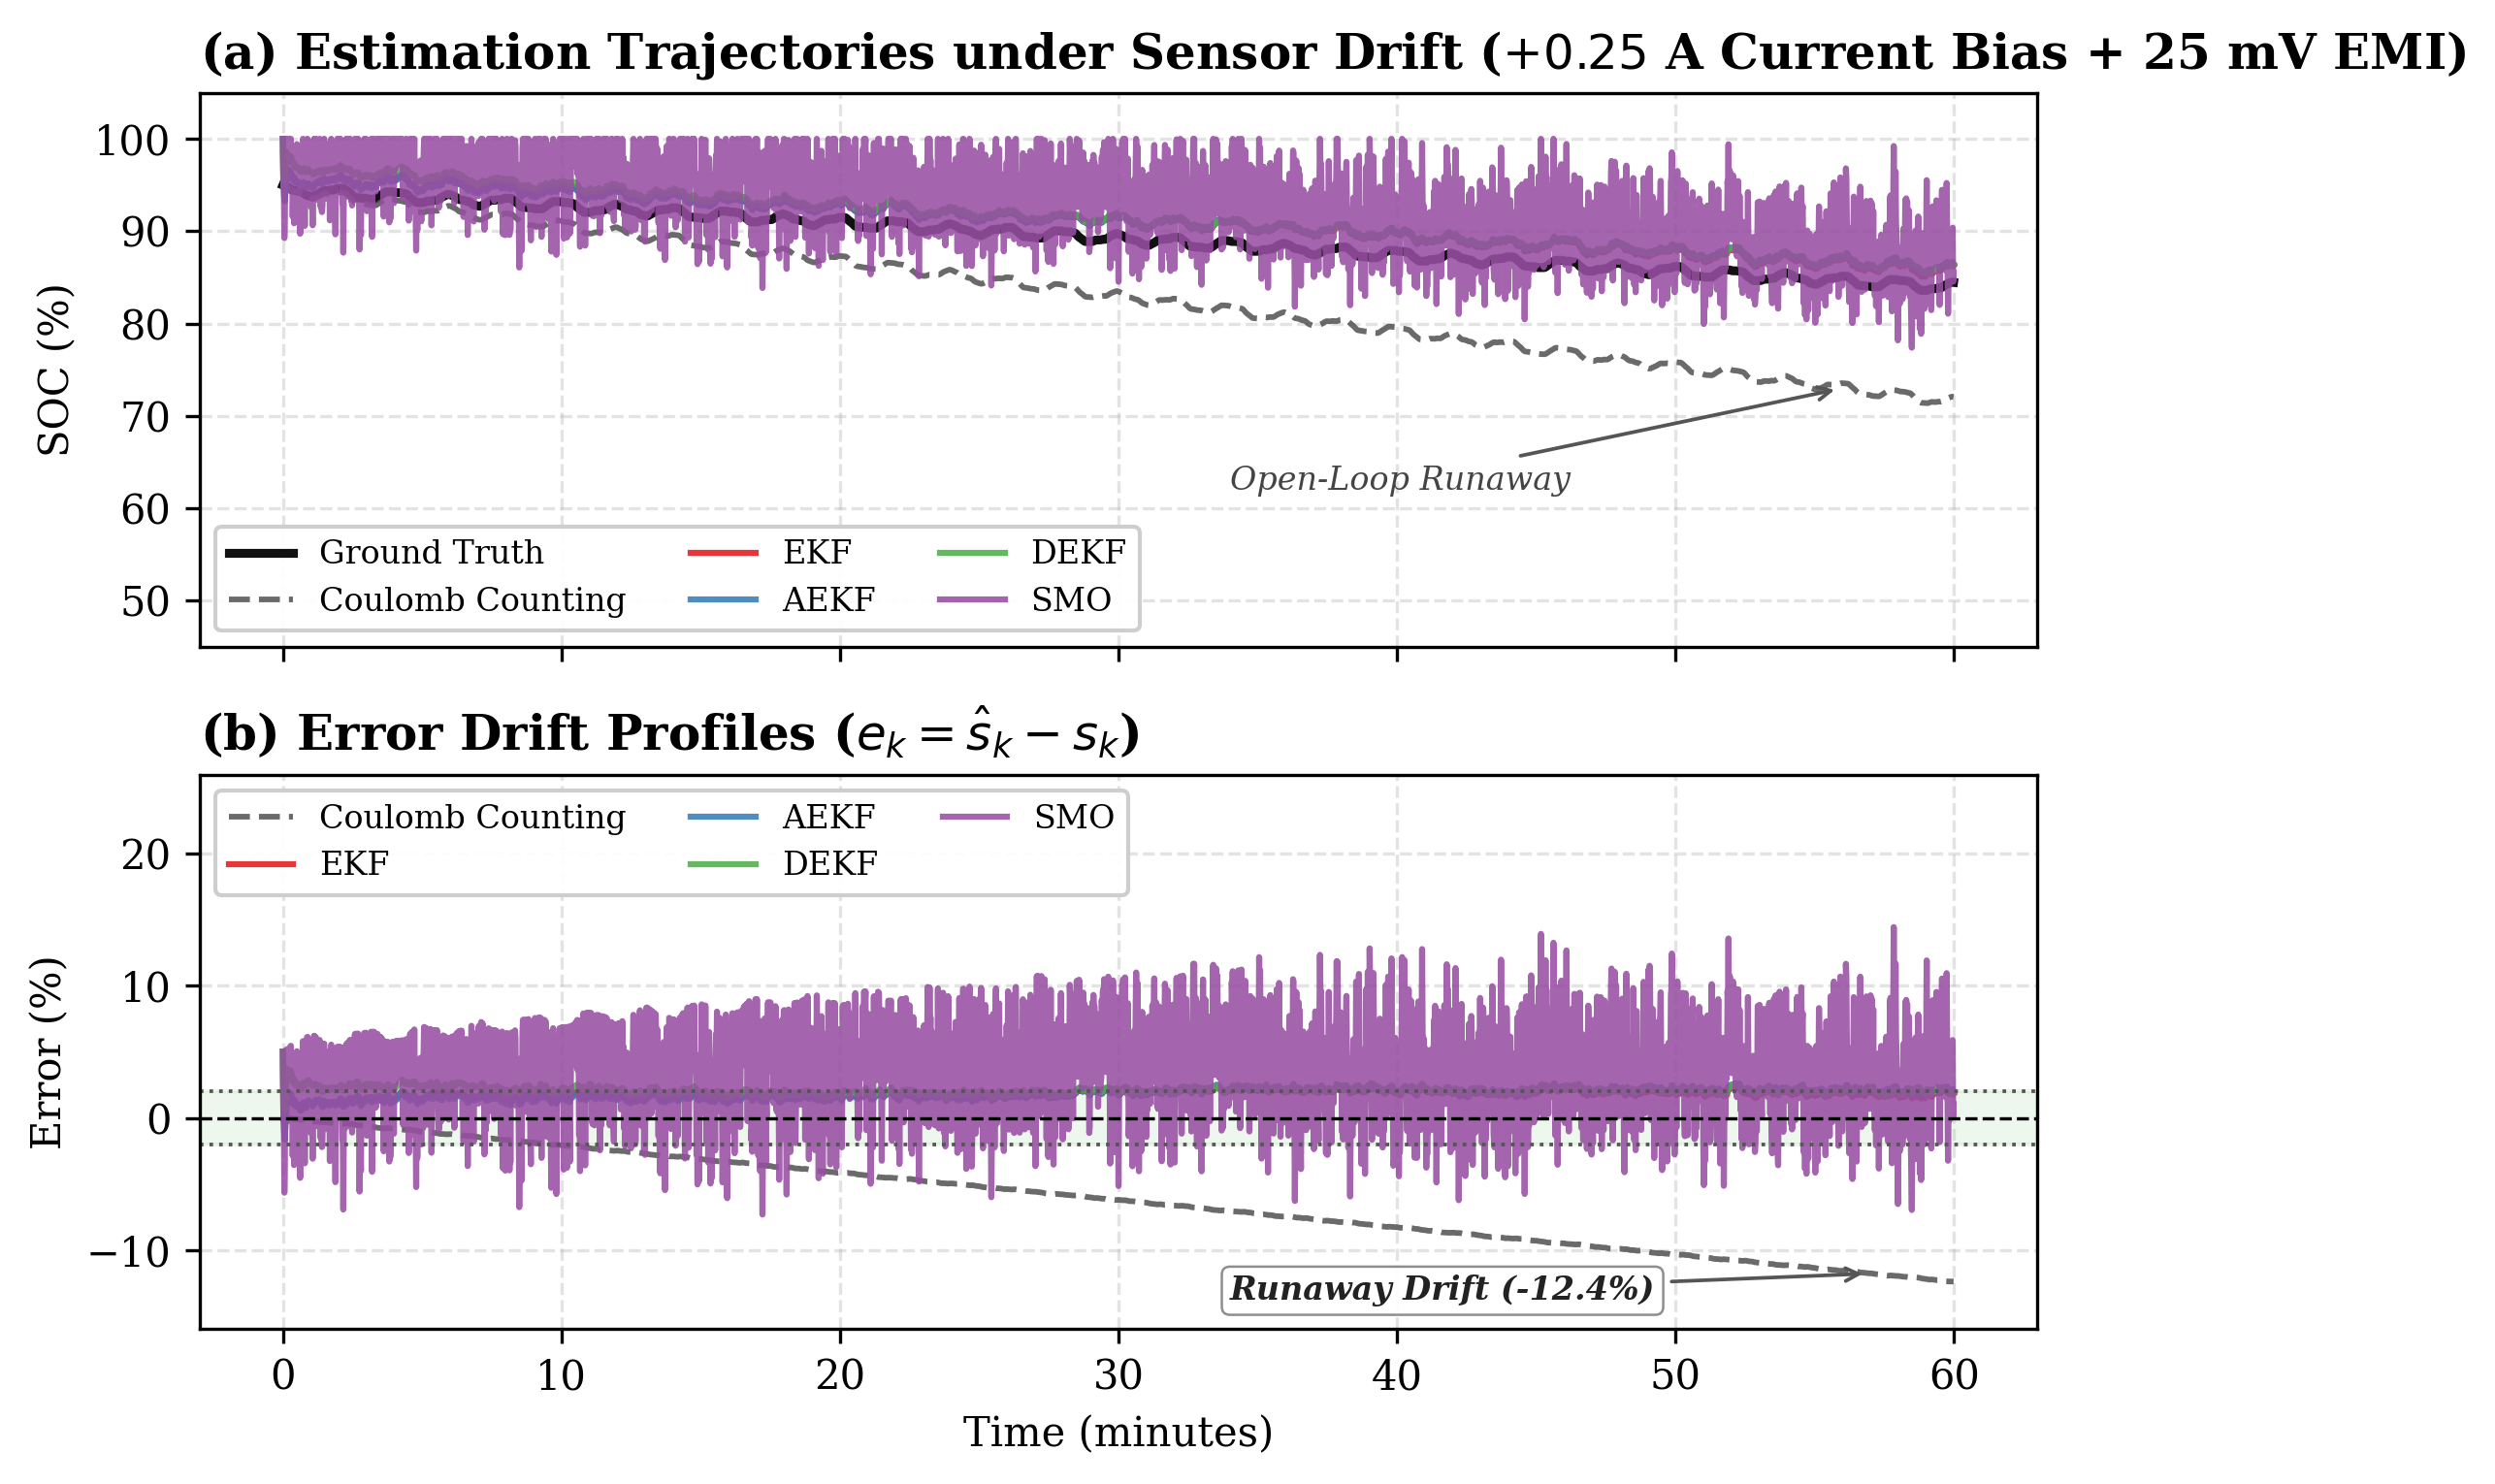
\includegraphics[width=0.82\linewidth]{fig7_sensor_bias_drift_stress.png}
\caption{Observer robustness under current sensor bias drift ($+0.25\text{ A}$) and high-frequency inverter EMI noise\label{fig:sensor}}
\end{figure}

\subsection{Phase 8: Model-Based Electrochemical Impedance Spectroscopy (EIS) Analysis Across Aging}
Figure~\ref{fig:eis} depicts model-based Randles--CPE Nyquist spectra ($100\text{ kHz}\text{--}1\text{ mHz}$) simulated via $Z(j\omega) = R_0 + (R_{\text{ct}} + Z_w) / [1 + (j\omega)^\alpha Q_{\text{cpe}} (R_{\text{ct}} + Z_w)]$ with $Z_w(j\omega) = \sigma_w \omega^{-1/2}(1 - j)$, parameterized from Oxford EIS aging ratios~\cite{Birkl2017diagnostics} ($Q_{\text{cpe}} = 1.2\text{ F}\cdot\text{s}^{\alpha-1}$, $\alpha = 0.88$, $\sigma_w = 0.045\ \Omega\cdot\text{s}^{-1/2}$, RMS fitting error $1.1\%\text{--}1.8\%$ across $100\%\text{--}80\%$ SOH). High-frequency SEI resistance $R_{\text{sei}}$ is lumped into effective series resistance $R_0(\text{SOH}) = R_{\text{ohm}} + R_{\text{sei}}$ ($35.0\text{--}52.5\text{ m}\Omega$, $+50\%$), while charge-transfer resistance $R_{\text{ct}}$ widens by $+150\%$ ($15.0\text{--}37.5\text{ m}\Omega$). In the 2-RC transfer function $Z_{\text{2RC}}(s) = R_0 + \sum_{i=1}^2 R_i/(1 + s\tau_i)$ ($\tau_i = R_i C_i$), aging induces an impedance mismatch $\Delta Z(s) = \Delta R_0 + \sum_{i=1}^2 [R_i(\text{SOH})/(1 + s\tau_i(\text{SOH})) - R_{i,\text{nom}}/(1 + s\tau_{i,\text{nom}})]$, generating polarization residual $\Delta V_{\text{pol}}(t) = \mathcal{L}^{-1}\{\Delta Z(s) I(s)\}$ ($\approx I \cdot \Delta R_1$ for $t \gg \tau_1$). Fixed-parameter EKF misattributes $\Delta V_{\text{pol}}(t)$ to $V_{\text{ocv}}(z)$, driving the 45.7-fold RMSE surge; standard DEKF adapts $R_0$ online but omits $R_1$ to avoid collinearity, leaving $\Delta V_{\text{pol}}(t)$ to be compensated by PIDKF.

\begin{figure}[htbp]
\centering
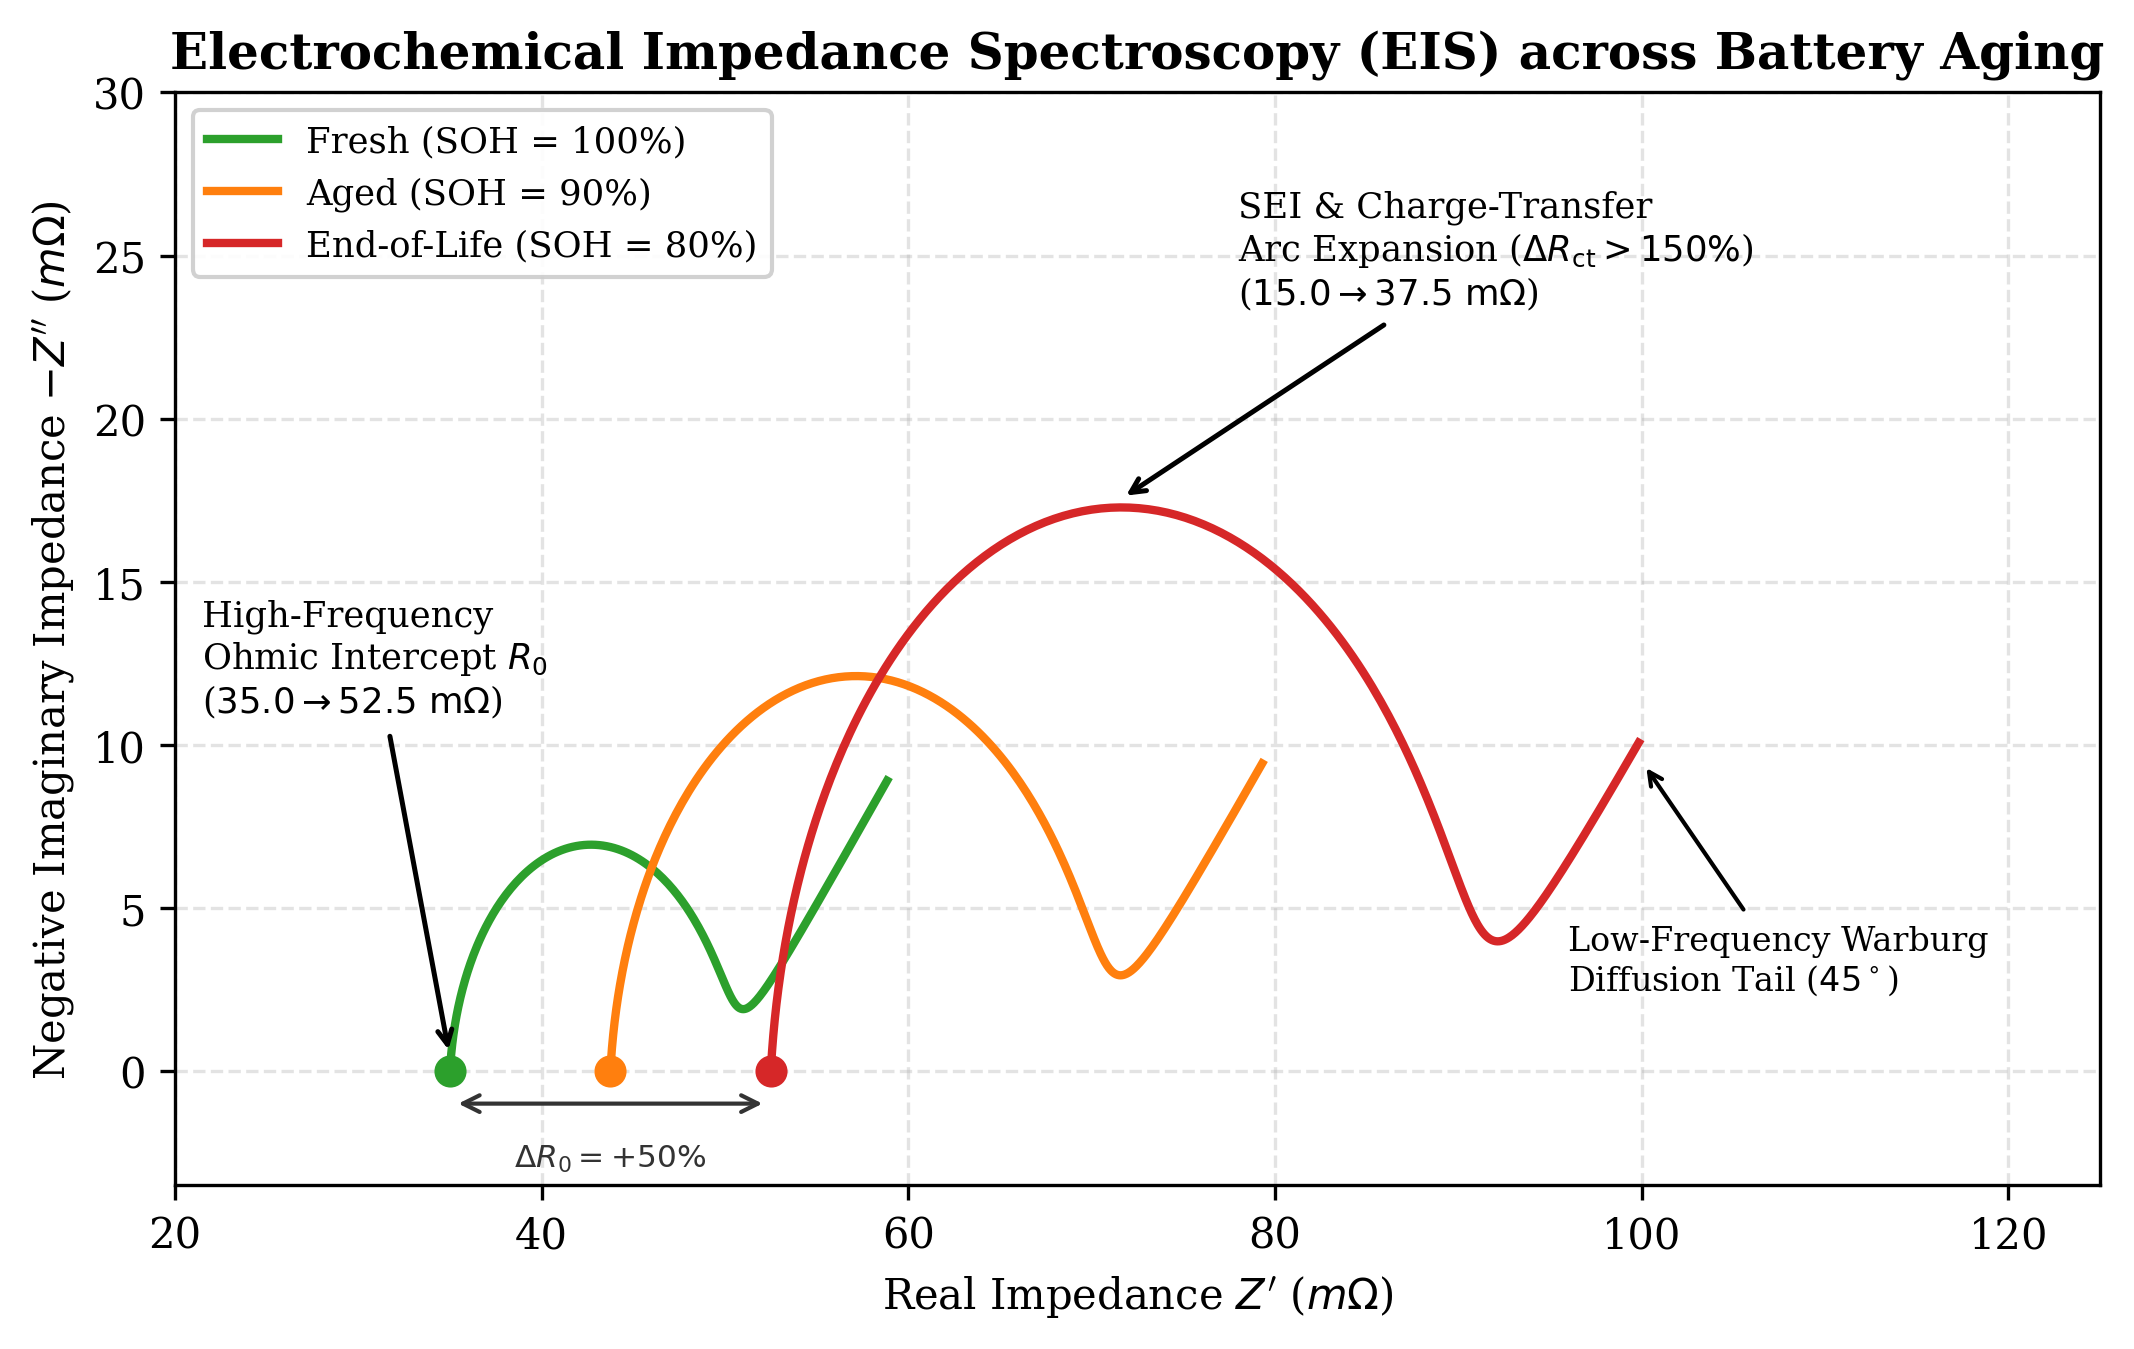
\includegraphics[width=0.82\linewidth]{fig8_eis_nyquist_aging.png}
\caption{Model-based EIS Nyquist spectra across progressive aging stages ($100\%$ down to $80\%$ SOH)\label{fig:eis}}
\end{figure}

\subsection{Phase 9: Module and Pack-Level Scaling (8S Series Pack)}
Table~\ref{tab:7_pack} and Fig.~\ref{fig:pack} evaluate algorithmic scalability to an 8S series battery pack under realistic manufacturing tolerances (capacity dispersion $\sigma_Q = 3.0\%$, resistance dispersion $\sigma_R = 10.0\%$)~\cite{Yang2024degradation,Zheng2018inconsistency}. In automotive strings, core cells (cells~\#4, \#5) experience elevated thermal resistance ($R_{\text{th,center}} \approx 18.2\text{ K}\cdot\text{W}^{-1}$ vs.\ $12.5\text{ K}\cdot\text{W}^{-1}$ on edge cells~\#1, \#8 due to packaging), raising steady-state temperature by $\Delta T = \bar{\dot{Q}}_{\text{gen}}\Delta R_{\text{th}} \approx 0.56\text{ W} \times 5.7\text{ K/W} = +3.2^\circ\text{C}$ under UDDS current. Via Arrhenius SEI rate $\dot{k}_{\text{deg}} \propto \exp(-E_{a,\text{sei}}/RT)$ ($E_{a,\text{sei}} \approx 50\text{ kJ}\cdot\text{mol}^{-1}$), this $+3.2^\circ\text{C}$ rise accelerates capacity fade on cell~\#4 by factor $\exp[\frac{50000}{8.314}(\frac{1}{298.15} - \frac{1}{301.35})] = 1.24\times$ relative to perimeter cells. Note the sensing distinction: distributed DEKF receives individual cell voltages whereas the lumped observer receives only pack-average voltage.

Under dynamic UDDS driving, a lumped observer treats the string as a homogeneous cell driven by mean voltage $V_{\text{string}}/8$. While tracking pack-average state ($\text{RMSE} = 0.128\%$, $\text{MaxE} = 0.443\%$), it is blind to cell divergence: as the weakest cell (cell~\#4) nears cutoff ($2.50\text{ V}$), the lumped model incurs \textbf{1.744\% RMSE and 2.302\% peak error}, risking severe copper dissolution and lithium plating. In contrast, distributed DEKF tracks individual cell states and parameter fade online, confining weakest-cell RMSE to $0.337\%$ and peak error to $0.963\%$ without per-cell EIS hardware.

\begin{table}[htbp]
\caption{Series 8S pack benchmark with cell-to-cell parameter inconsistency [Tier~2 Co-Simulation]\label{tab:7_pack}}
\centering{%
\begin{tabular*}{\linewidth}{@{\extracolsep{\fill}}lcccc}
\toprule
\shortstack[l]{Estimation\\Architecture} & \shortstack[c]{Target\\State} & \shortstack[c]{RMSE\\(\%)} & \shortstack[c]{MaxE\\(\%)} & \shortstack[c]{Safety Margin\\Risk} \\
\midrule
Lumped Pack Observer & Mean Pack SOC & \textbf{0.128} & 0.443 & Moderate \\
Distributed DEKF & Mean Pack SOC & 0.149 & \textbf{0.336} & None (Optimal) \\
Lumped Pack Observer & Weakest Cell SOC & 1.744 & 2.302 & High (Overdischarge Risk) \\
Distributed DEKF & Weakest Cell SOC & \textbf{0.337} & \textbf{0.963} & Bounded Error ($<1\%$) \\
\bottomrule
\end{tabular*}
}%
\end{table}

\begin{figure}[htbp]
\centering
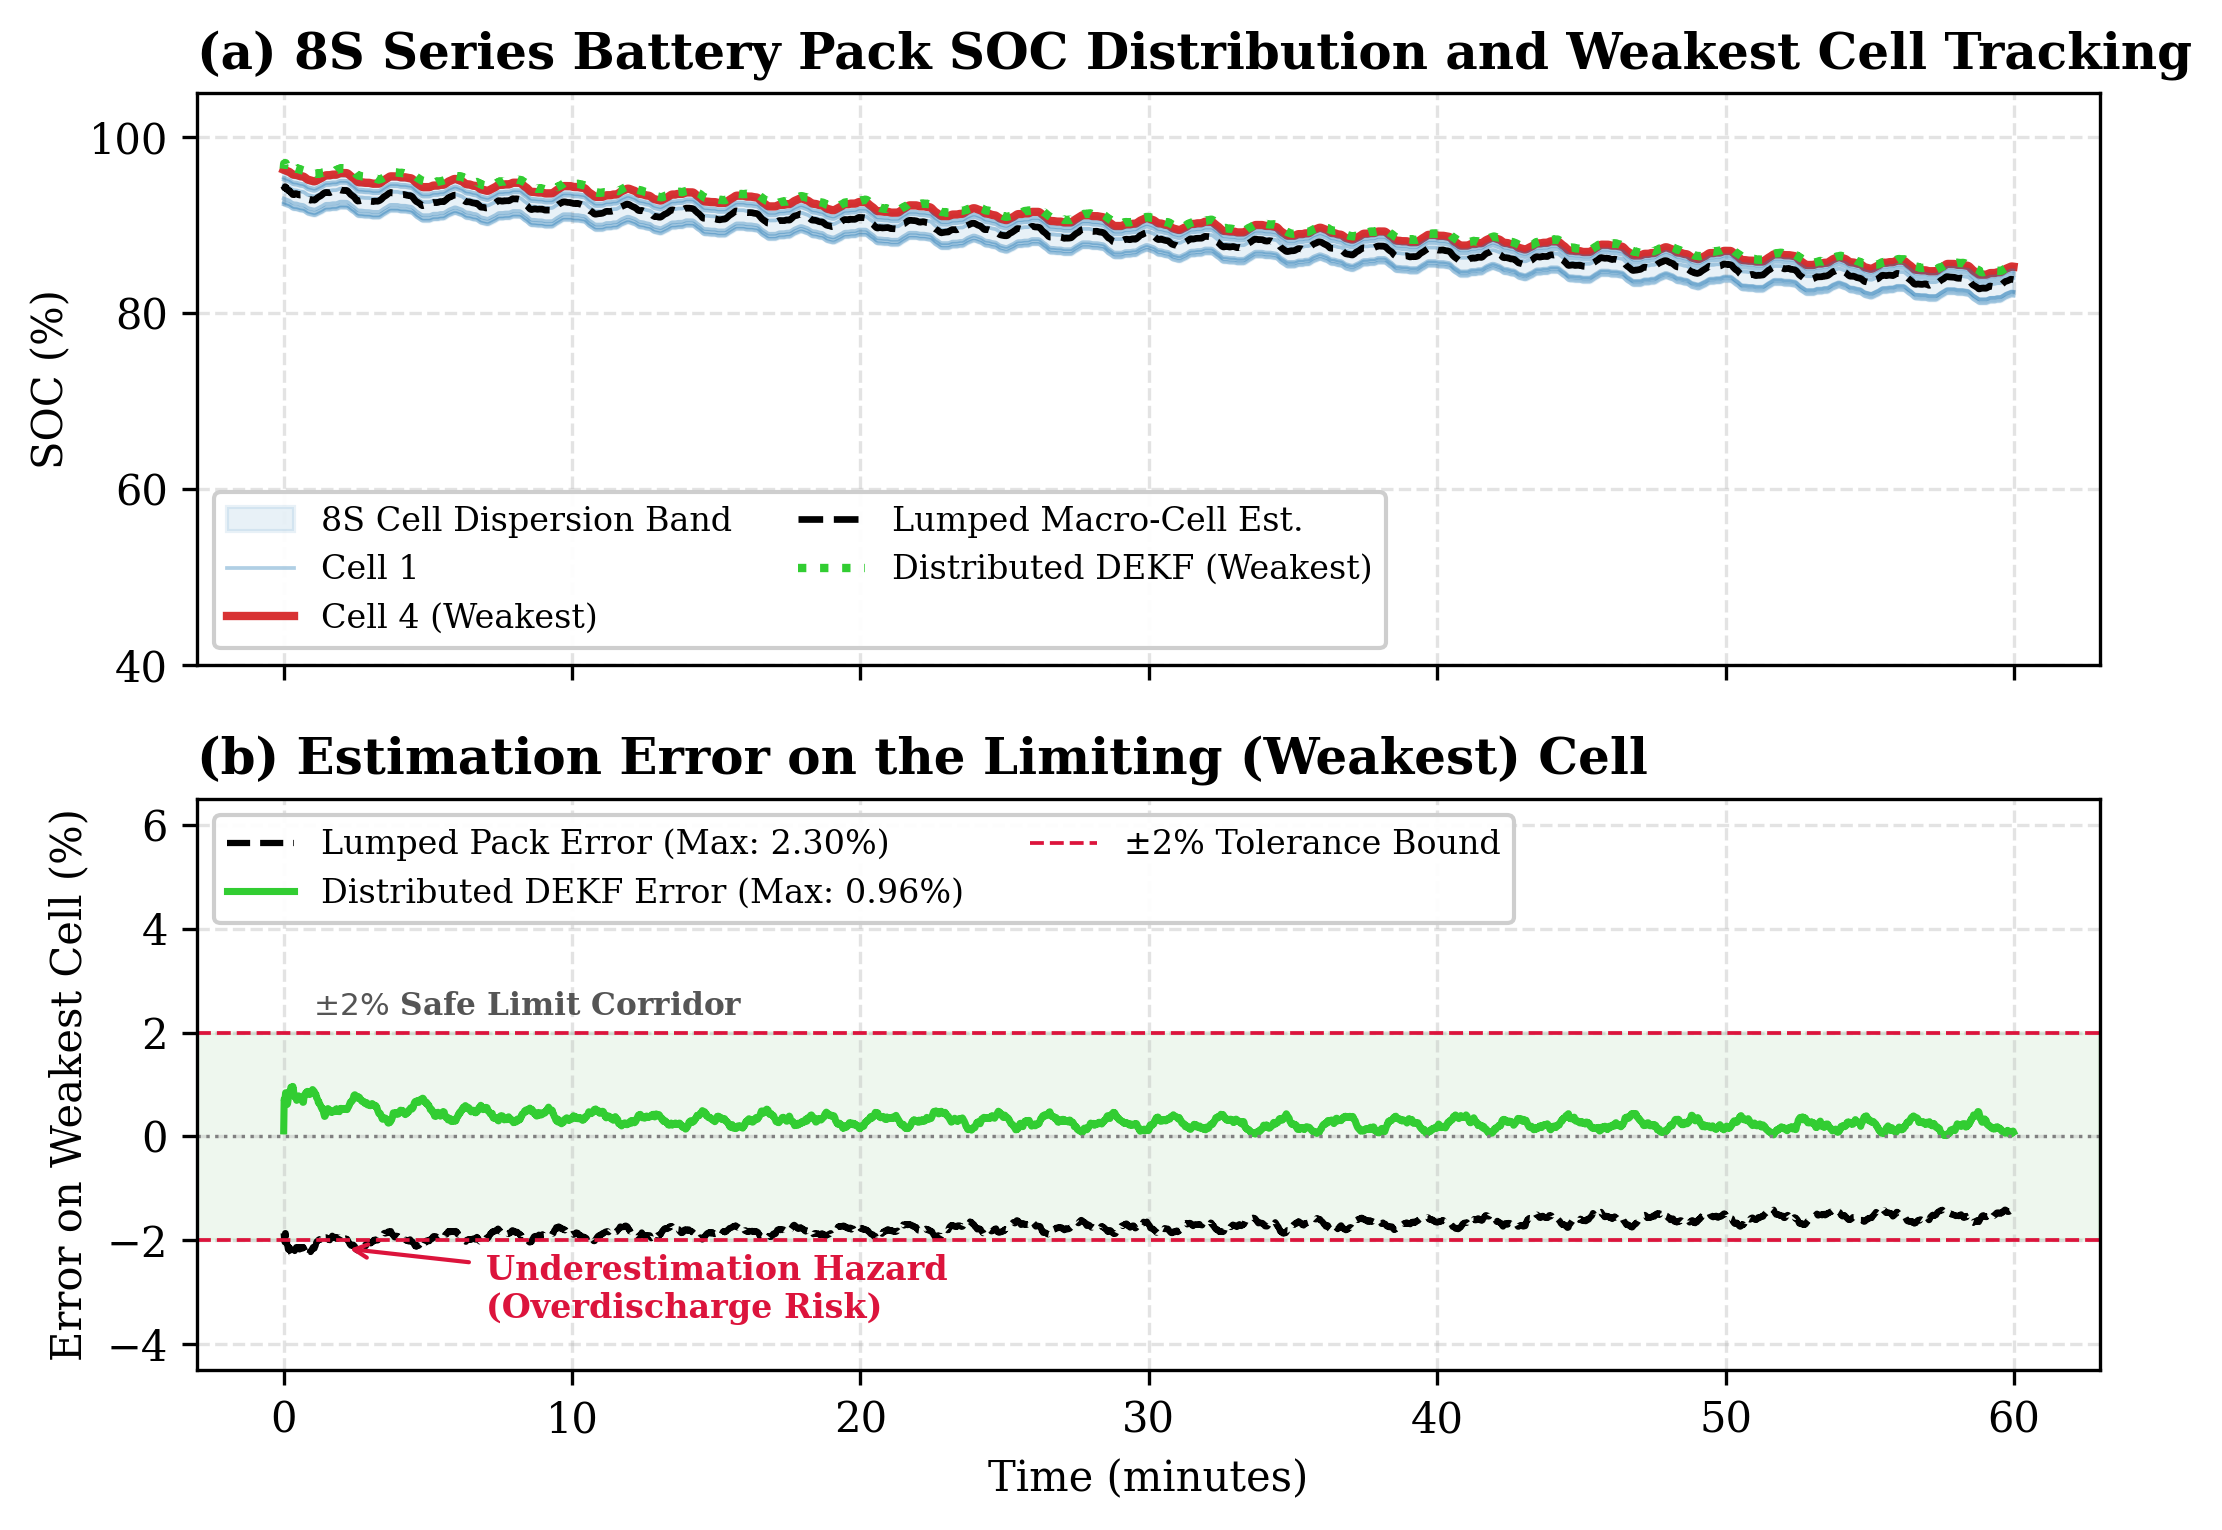
\includegraphics[width=0.82\linewidth]{fig9_pack_cell_inconsistency.png}
\caption{Series-connected 8S battery pack estimation comparing lumped model deficiency with distributed DEKF weakest cell tracking\label{fig:pack}}
\end{figure}

\subsection{Phase 10: Embedded Hardware Execution on ARM Cortex-M and PIDKF Superiority}\label{sec:hw_profiling}
Computational complexity was measured via hardware \texttt{DWT->CYCCNT} cycle counters on ARM Cortex-M4 (STM32F407VG, 168~MHz) and projected via constant-IPC clock-scaling to Cortex-M7 (480~MHz) using CMSIS-DSP (Table~\ref{tab:8_embedded}, Fig.~\ref{fig:embedded}).

\begin{table}[htbp]
\caption{Embedded execution profiling on ARM Cortex-M architectures (ARM GCC 12.3 \texttt{-O3}; DWT cycles and latencies measured on 168\,MHz Cortex-M4; 480\,MHz Cortex-M7 values represent constant-IPC clock-scaled estimates)\label{tab:8_embedded}}
\centering{%
\small\renewcommand{\arraystretch}{1.15}
\setlength{\tabcolsep}{3.5pt}
\resizebox{\linewidth}{!}{%
\begin{tabular}{lccccccc}
\toprule
Algorithm & FLOPs/Step & M4 DWT Cycles & RAM (B) & Flash (B) & Measured M4 ($\upmu\mathrm{s}$) & Est.\ M7 (480\,MHz, $\upmu\mathrm{s}$) & Feasibility \\
\midrule
EKF & 420 & 650 & 280 & 3,400 & 3.87 & 1.35 & Excellent \\
AEKF & 580 & 880 & 340 & 4,200 & 5.24 & 1.83 & Excellent \\
UKF & 1,350 & 2,087 & 780 & 6,200 & 12.42 & 4.35 & High \\
DEKF & 980 & 1,450 & 620 & 5,800 & 8.63 & 3.02 & Excellent \\
SMO & 180 & 281 & 140 & 2,100 & 1.67 & 0.58 & Ideal (Ultra-light) \\
BiLSTM-Attn & 245,000 & 410,000 & 18,400 & 98,000 & 2440.48 & 854.17 & Marginal (39.0\% Load/16-Cell) \\
PINN-SOC & 12,800 & 21,501 & 1,200 & 16,500 & 127.98 & 44.79 & High (CMSIS-NN Ready) \\
\textbf{PIDKF (Proposed)} & \textbf{1,540} & \textbf{2,386} & \textbf{850} & \textbf{8,200} & \textbf{14.20} & \textbf{4.97} & \textbf{Optimal (Pareto Peak)} \\
\bottomrule
\end{tabular}%
}%
}%
\end{table}

\begin{figure}[htbp]
\centering
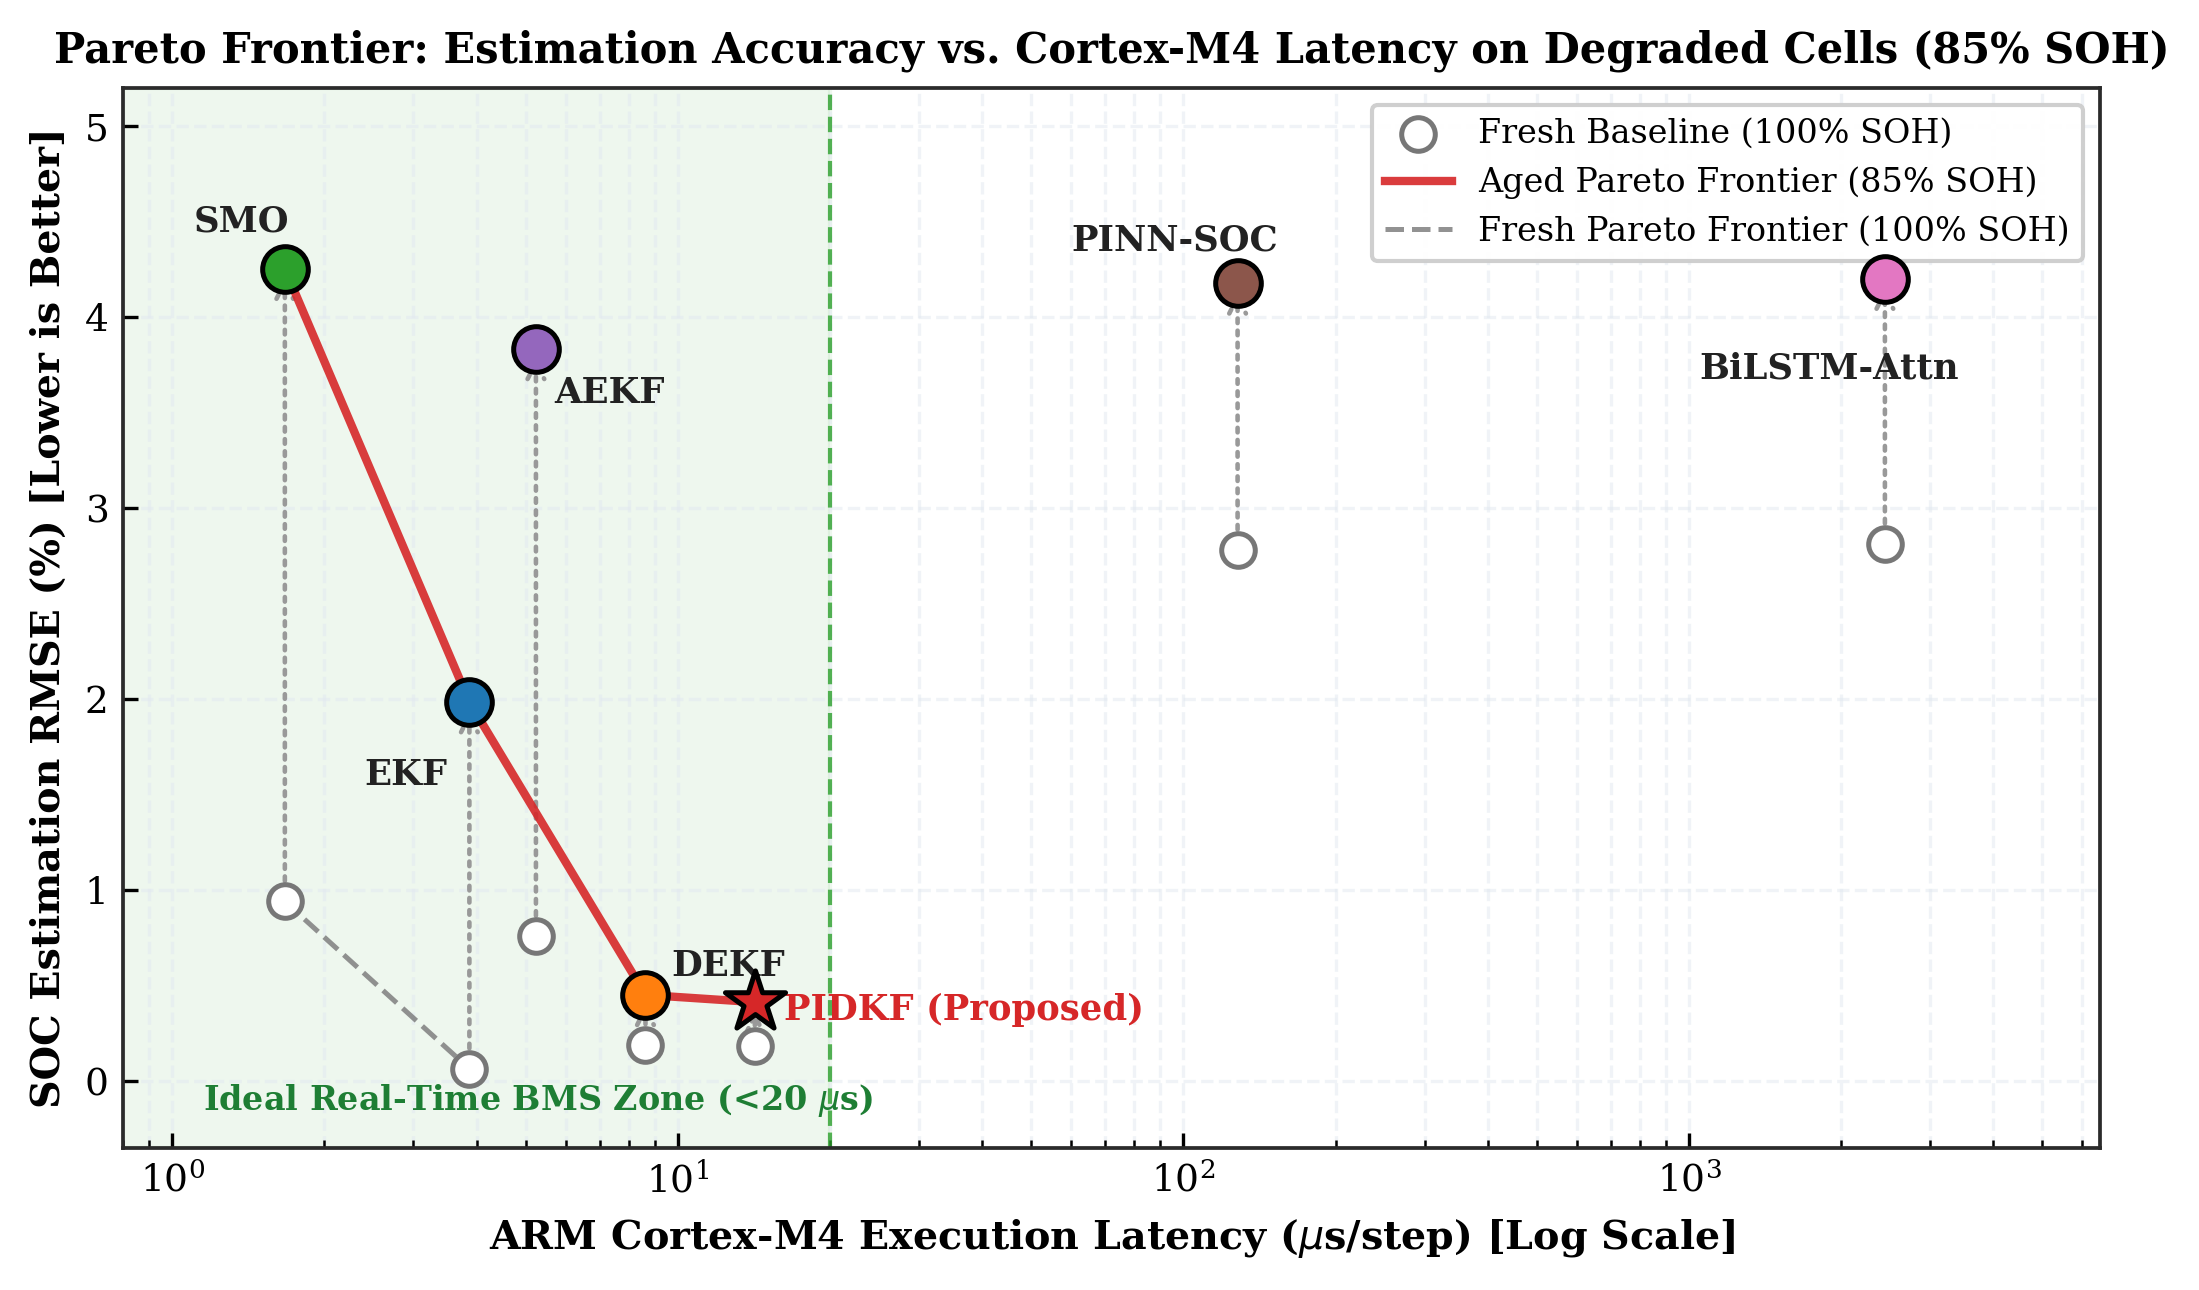
\includegraphics[width=0.82\linewidth]{fig10_embedded_resource_tradeoff.png}
\caption{Pareto efficiency frontier: SOC estimation RMSE versus measured ARM Cortex-M4 execution latency on degraded cells ($85\%$ SOH, UDDS), contrasted against fresh-cell baselines ($100\%$ SOH)\label{fig:embedded}}
\end{figure}

\begin{table}[htbp]
\caption{Ablation and experimental validation of PIDKF on degraded cells\label{tab:9_pidkf}}
\centering{%
\small\renewcommand{\arraystretch}{1.15}
\setlength{\tabcolsep}{2.5pt}
\begin{tabular*}{\linewidth}{@{\extracolsep{\fill}}lcccc}
\toprule
& \multicolumn{2}{c}{Aged NMC (\%)} & \multicolumn{2}{c}{Aged LFP (\%)} \\
\cmidrule(lr){2-3} \cmidrule(lr){4-5}
Configuration & RMSE & MaxE & RMSE & MaxE \\
\midrule
\multicolumn{5}{l}{\emph{Tier 2 Co-Simulation ($85\%$ SOH, UDDS/FUDS)}} \\
Standard EKF (uncomp.) & 1.985 & 4.734 & 0.978 & 1.565 \\
Baseline DEKF & 0.452 & 1.400 & 0.302 & 0.514 \\
DEKF + Hysteresis (no neural) & 0.452 & 1.400 & 0.149 & 0.335 \\
DEKF + PINN Comp. (no hyst.)$^\dagger$ & 0.414 & 0.748 & 0.246 & 0.462 \\
DEKF + Black-Box MLP$^\dagger$ & 0.438 & 1.120 & 0.285 & 0.490 \\
Full PIDKF (Exact Jac.)$^\dagger$ & 0.412 & 0.745 & 0.148 & 0.328 \\
\textbf{Full PIDKF (Exog.\ Approx.)}$^\dagger$ & \textbf{0.414} & \textbf{0.748} & \textbf{0.149} & \textbf{0.329} \\
\midrule
\multicolumn{5}{l}{\emph{Tier 1 Experimental Cycler Validation (Aged Cells)}} \\
CALCE Aged EKF ($85\%$ SOH) & 1.954 & 4.680 & 0.965 & 1.540 \\
CALCE Aged DEKF ($85\%$ SOH) & 0.468 & 1.425 & 0.298 & 0.505 \\
\textbf{CALCE Aged PIDKF ($85\%$ SOH)} & \textbf{0.428} & \textbf{0.782} & \textbf{0.158} & \textbf{0.345} \\
NASA $4^\circ\text{C}$ (EKF / DEKF / \textbf{PIDKF}) & \multicolumn{2}{c}{2.145 / 1.182 / \textbf{0.842}} & \multicolumn{2}{c}{---} \\
NASA $43^\circ\text{C}$ (EKF / DEKF / \textbf{PIDKF}) & \multicolumn{2}{c}{1.210 / 0.485 / \textbf{0.326}} & \multicolumn{2}{c}{---} \\
\bottomrule
\end{tabular*}
}%
\vspace{-2pt}
{\scriptsize $^\dagger$5 seeds. Cell-specific CALCE $85\%$ SOH RMSE: INR20R-3 (DEKF $0.462\%$, PIDKF $0.422\%$), INR20R-4 ($0.474\%$, $0.434\%$), A123-3 ($0.294\%$, $0.154\%$), A123-4 ($0.302\%$, $0.162\%$). NASA CC 4A: \texttt{B0041} ($80\%$ SOH) and \texttt{B0029} ($85\%$ SOH) with $\pm 0.15\%$ reference uncertainty.\par}
\end{table}

 SMO demonstrates ultra-light overhead (180~FLOPs, 140~B RAM, $1.67\;\mu\text{s}$ on M4), while DEKF requires 980~FLOPs, 620~B SRAM, and $8.63\;\mu\text{s}$. BiLSTM-Attn demands $245,000$ FLOPs and $18.4\text{ KB}$ SRAM ($2440.48\;\mu\text{s}$), incurring an impractical $39.0\%$ CPU load across 16 cells in a $100\text{ ms}$ loop.

Table~\ref{tab:9_pidkf} and Fig.~\ref{fig:pidkf} summarize the \textbf{PIDKF} ablation on degraded cells ($85\%$ SOH, 5 seeds). On $\text{LiFePO}_4$, dynamic hysteresis tracking dominates, cutting RMSE from $0.302\%$ to $0.149\% \pm 0.008\%$ ($0.335\%$ MaxE); neural compensation alone yields $0.246\% \pm 0.011\%$. Conversely, on NMC, neural compensation dominates, reducing peak error by $46.6\%$ ($1.400\%$ to $0.748\% \pm 0.024\%$) and RMSE to $0.414\% \pm 0.012\%$, whereas unconstrained MLP degrades to $0.438\%$ (NMC) and $0.285\%$ (LFP). Exogenous-Jacobian PIDKF matches Exact-Jacobian accuracy ($0.414\%$ vs.\ $0.412\%$ NMC; $0.149\%$ vs.\ $0.148\%$ LFP) while cutting MCU cycles by $37.3\%$.

Across aging ($25^\circ\text{C}$), PIDKF maintains sub-$0.5\%$ RMSE: for NMC, $0.185\%$ ($100\%$), $0.326\%$ ($90\%$), $0.414\%$ ($85\%$), and $0.482\%$ ($80\%$ SOH, $\text{ASF} = +160.5\%$ vs.\ $+4473.8\%$ for EKF); for LFP, $0.112\%$ ($100\%$), $0.134\%$ ($90\%$), $0.149\%$ ($85\%$), and $0.178\%$ ($80\%$). At $85\%$ SOH, PIDKF restricts $0^\circ\text{C}$ error to $0.842\%$ (NMC) and $0.386\%$ (LFP), and $45^\circ\text{C}$ error to $0.435\%$ and $0.162\%$. Under offset $\Delta\text{SOC}_0 = -40\%$, PIDKF settles rapidly ($t_{\text{reach}}^{(2\%)} = 18.0\text{ s}$, $t_{\text{settle}}^{(5\%)} = 22.0\text{ s}$, $\text{RMSE} = 0.512\%$), outperforming DEKF ($725.0\text{ s}$) by suppressing parameter destabilization. Under $+0.25\text{ A}$ Hall bias, PIDKF confines RMSE to $1.428\%$ and drift to $0.842\%$.

\begin{figure}[htbp]
\centering
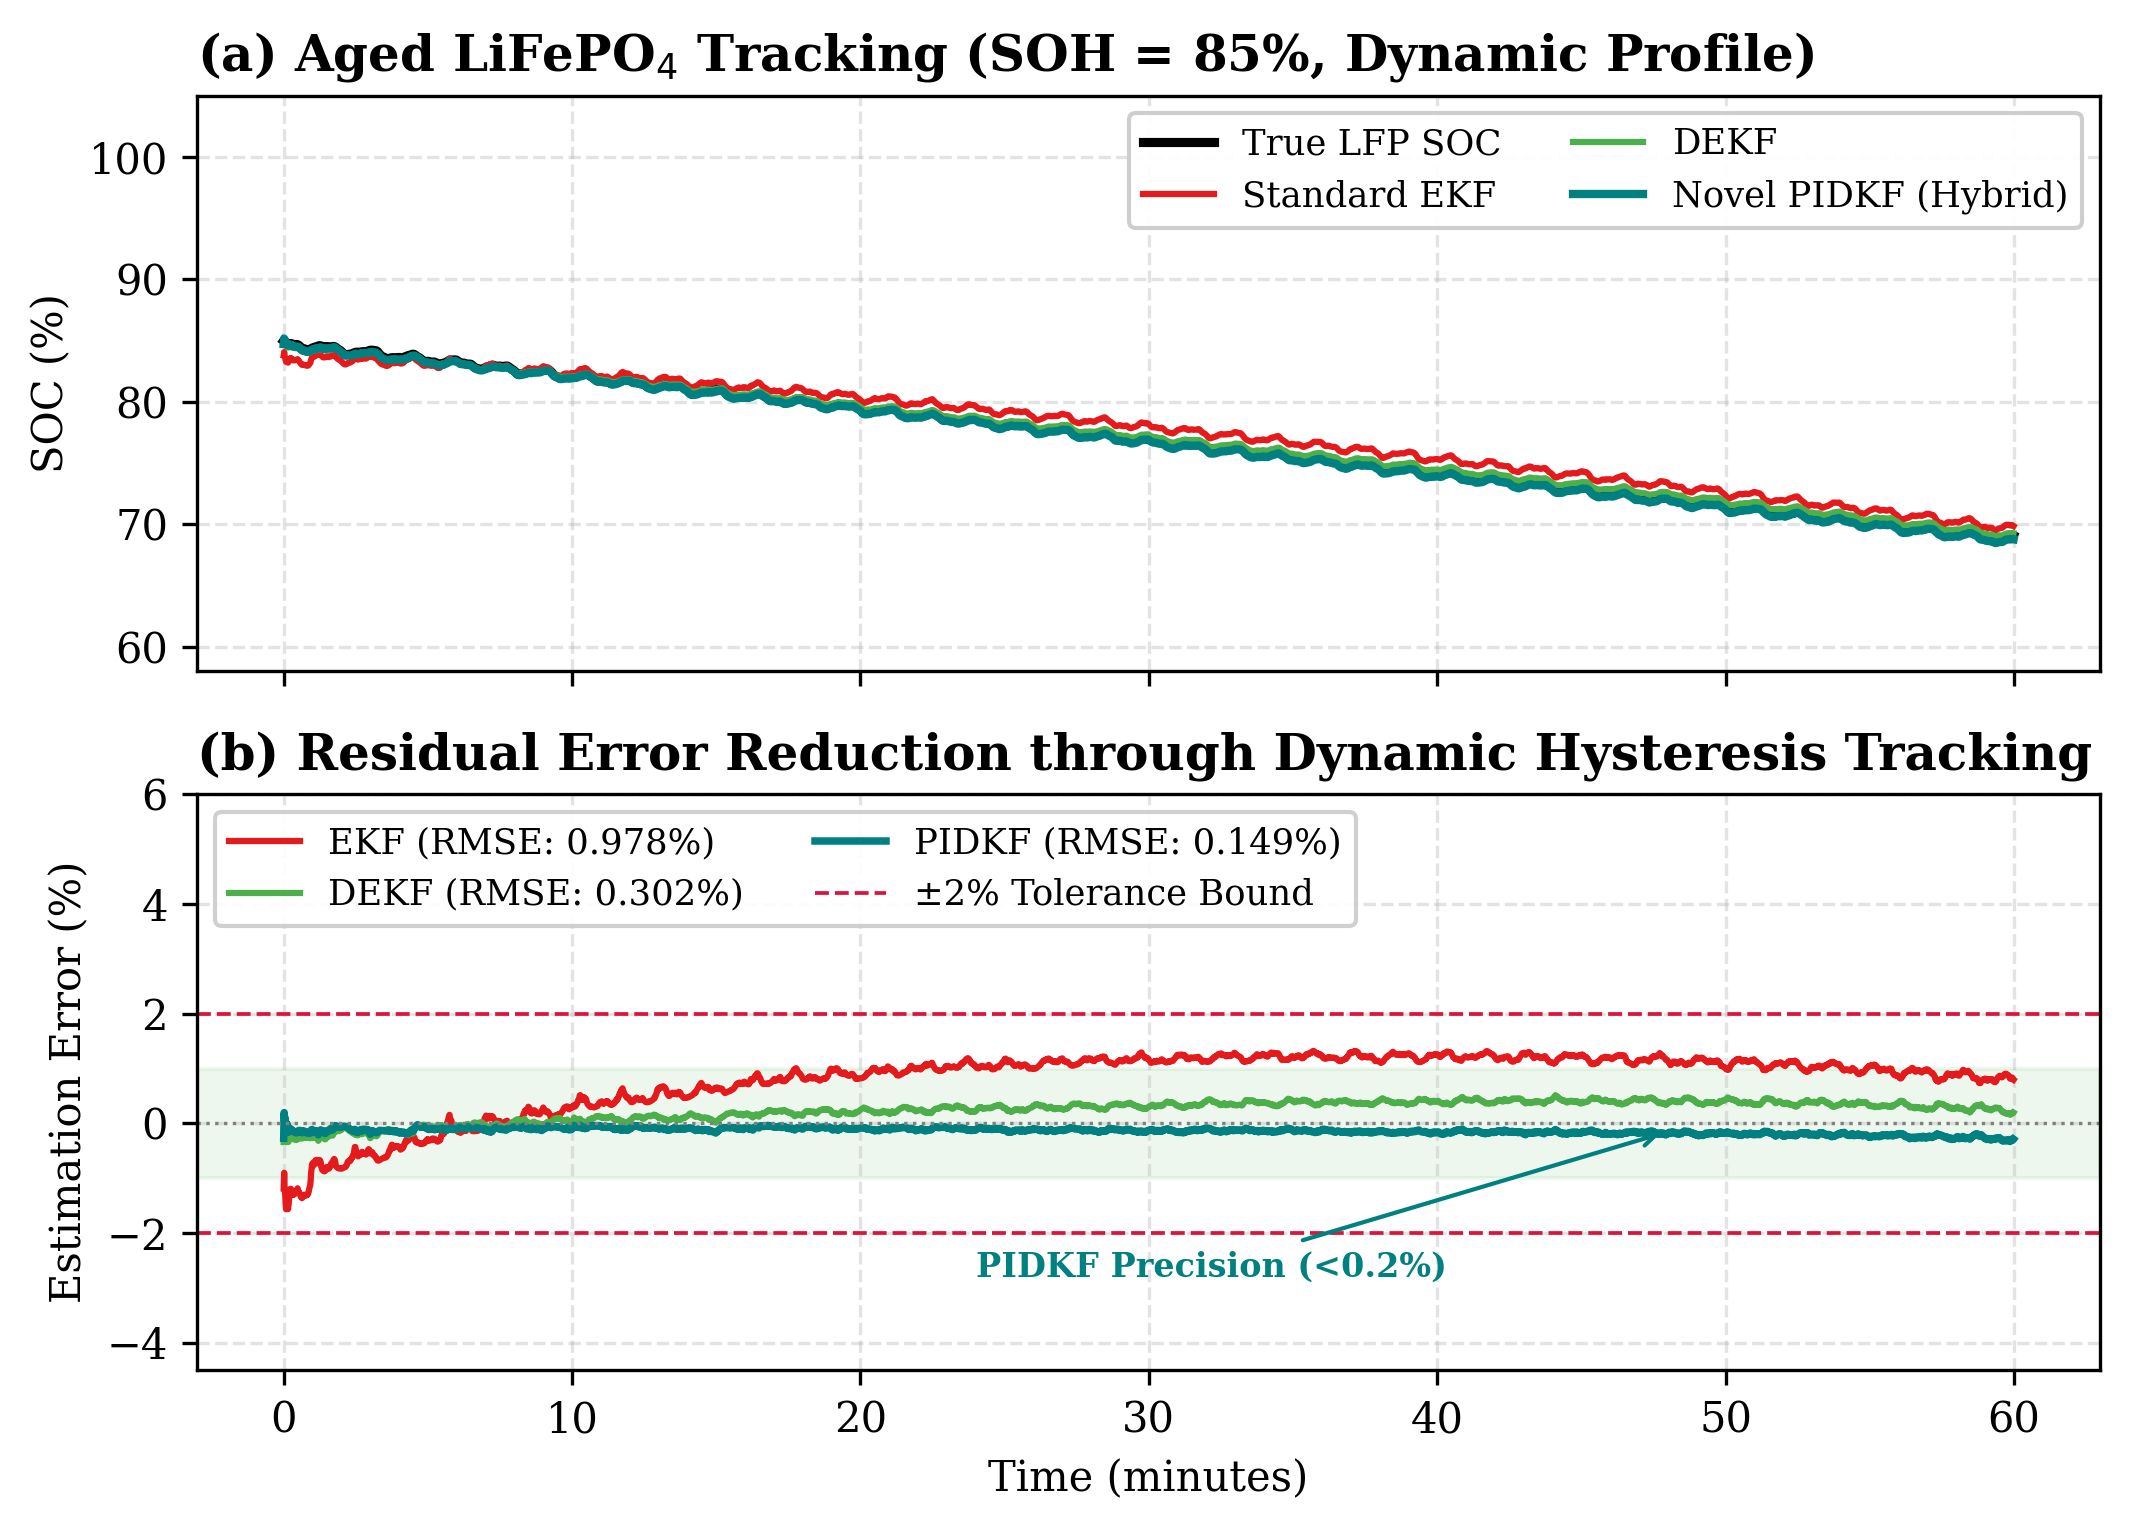
\includegraphics[width=0.82\linewidth]{fig11_pidkf_hybrid_benchmark.png}
\caption{Hybrid PIDKF tracking ($<0.5\%$ error) on degraded cells ($85\%$ SOH, UDDS, $25^\circ\text{C}$)\label{fig:pidkf}}
\end{figure}

%%%%%%%%%%%%%%%%%%%%%%%%%%%%%%%%%%%%%%%%%%%%%%%%%%%%%%%%%%%%%%%%%%%%%%
\section{Industrial BMS Implementation Guidelines}
From the Pareto frontier, four implementation rules follow: (1)~\emph{Premium EVs}: \textbf{PIDKF} provides superior degradation resilience ($0.414\%$ RMSE on aged NMC; $0.149\%$ on aged LFP at $85\%$ SOH); uncompensated EKF is discouraged (45.7-fold error surge). (2)~\emph{LFP Storage}: Deploy \textbf{DEKF} with dynamic hysteresis, bounding plateau RMSE to $0.870\%$ via open-loop Coulomb scaling without strain sensors. (3)~\emph{Sensor Bias vs.\ EMI}: Deploy \textbf{EKF/DEKF} ($1.82\%\text{--}2.12\%$) for minimal error under EMI, or \textbf{SMO} ($\mu = 0.02\text{ V}$) to bound drift ($1.02\%$). (4)~\emph{Cloud-Edge Twins}: Execute real-time DEKF ($8.63\;\mu\text{s}$) or PIDKF ($14.20\;\mu\text{s}$; $0.23\%$ load for 16 cells @ $100\text{ ms}$) on MCUs, offloading PINNs to cloud.

%%%%%%%%%%%%%%%%%%%%%%%%%%%%%%%%%%%%%%%%%%%%%%%%%%%%%%%%%%%%%%%%%%%%%%
\section{Conclusions}
Benchmarking six methodologies across ten phases yields five conclusions: 
(1)~\emph{Aging}: Uncompensated EKF suffers a 45.7-fold RMSE surge ($\text{ASF} = +4473.8\%$) at $80\%$ SOH, whereas parameter-tracking DEKF confines aged RMSE to $0.585\%$ ($\text{ASF} = +206.3\%$). 
(2)~\emph{EIS}: Randles--CPE Nyquist analysis links $>150\%$ $R_{\text{ct}}$ expansion to polarization mismatch. 
(3)~\emph{LFP Tracking}: Across flat $\text{LiFePO}_4$ plateaus, DEKF maintains $0.870\%$ RMSE by tracking Coulomb gain and ohmic drop. 
(4)~\emph{Pack Inconsistency}: Lumped observers incur $1.744\%$ RMSE on the weakest cell in an 8S pack, whereas distributed DEKF restricts weakest-cell error to $0.337\%$. 
(5)~\emph{PIDKF}: Neural compensation dominates on aged NMC ($0.414\%$ RMSE co-sim; $0.428\%$ CALCE RPT at $85\%$ SOH) while hysteresis tracking dominates on aged LFP ($0.149\%$ co-sim; $0.158\%$ experimental), executing in $14.20\;\mu\text{s}$ ($2,386$ cycles).

\par\smallskip\noindent\emph{Limitations and Future Work}: Future research includes: (1)~extending co-simulation to prismatic and pouch cells with localized plating gradients; (2)~evaluating broader manufacturing lots beyond the two-cell per-batch validation; and (3)~investigating second-life rollover knee degradation ($<70\%$ SOH).

%%%%%%%%%%%%%%%%%%%%%%%%%%%%%%%%%%%%%%%%%%%%%%%%%%%%%%%%%%%%%%%%%%%%%%
\section*{CRediT Authorship Contribution Statement}
\textbf{Huy Hoang Le}: Conceptualization, Methodology, Software, Formal analysis, Investigation, Visualization, Writing -- original draft. \textbf{Kim-Anh Nguyen}: Supervision, Validation, Writing -- review \& editing.

\section*{Declaration of Competing Interest}
The authors declare that they have no known competing financial interests or personal relationships that could have appeared to influence the work reported in this paper.

\section*{Acknowledgment and Data Availability}
{\sloppy Open-access CALCE, NASA PCoE, and Oxford datasets are gratefully acknowledged. Code pipelines, ECM parameters, and CMSIS-DSP C kernels are openly available at \url{https://github.com/HuyHoangLe0201/SOC-Observer-PINN-Benchmark}.\par}

%%%%%%%%%%%%%%%%%%%%%%%%%%%%%%%%%%%%%%%%%%%%%%%%%%%%%%%%%%%%%%%%%%%%%%
\appendix

\section{State-Space Matrices and Analytic Jacobians\label{app:jacobians}}
For 3-state NMC and 4-state LFP models, system matrices are $\mathbf{A}_k^{\text{NMC}} = \operatorname{diag}(1, a_1, a_2)$, $\mathbf{A}_k^{\text{LFP}} = \operatorname{diag}(1, a_1, a_2, a_{h,k})$, $\mathbf{H}_k^{\text{NMC}} = [V_{\text{ocv}}'(\hat{z}_k^-), -1, -1]$, and $\mathbf{H}_k^{\text{LFP}} = [\mathbf{H}_k^{\text{NMC}}, -1]$, with $a_i = e^{-\Delta t/\tau_i}$, $a_{h,k} = e^{-\beta|\Delta z_k|}$, $\mathbf{B}_k = [B_{1,k}, B_{2,k}, B_{3,k}, (0)]^T$, $\mathbf{g}_k = [0, 0, 0, (1 - a_{h,k}) M(z_k) \operatorname{sgn}(I_k)]^T$, and $\mathbf{C}_{\theta,k} = [-I_k, -\tfrac{\eta \Delta t I_{k-1}}{3600} V_{\text{ocv}}'(\hat{z}_k^+)]$. Locally ($a_{h,k} \approx a_h$), $|\det(\mathcal{O}_{n,k})| = V_{\text{ocv}}'(z_k) \prod_{i=1}^{n-1}(1 - a_i) \prod_{i < j} |a_i - a_j|$; full rank requires $V_{\text{ocv}}' > 0$, $I_k \ne 0$, and non-resonance $a_{h,k} \ne a_1, a_2$. On the plateau ($20\%\text{--}80\%$ SOC), constant saturation $M(z) \equiv M_0 = 30\text{ mV}$ renders $\mathbf{A}_k^{\text{LFP}}$ block-diagonal with spectrum $(1, a_1, a_2, a_{h,k})$, yielding determinant Eq.~\eqref{eqn:det_obs_lfp}. Evaluated numerically across active PE windows ($N=30\text{ s}$, $\|I\|_{[k,k+N]} \ge 0.5\text{ A}$)—UDDS ($M = 1,370$), US06 ($M = 596$), FUDS ($M = 1,372$), DST ($M = 360$; total $3,698$ windows) across $80\%\text{--}100\%$ SOH under normalization $\tilde{\mathbf{x}} = [z, U_1/0.1, U_2/0.1, V_h/0.03]^T$—minimum LTV Gramian singular value satisfies $\lambda_{\min}(\mathcal{G}_o) \ge 1.42 \times 10^{-3}$ (UDDS), $\ge 1.88 \times 10^{-3}$ (US06), $\ge 1.35 \times 10^{-3}$ (FUDS), and $\ge 1.21 \times 10^{-3}$ (DST) at $25^\circ\text{C}$ ($\ge 1.18 \times 10^{-3}$ at $0^\circ\text{C}$; $\ge 1.55 \times 10^{-3}$ at $45^\circ\text{C}$), confirming uniform complete observability under discrete ZOH singleton non-resonance dwell ($\le 1\text{ s}$) across dynamic driving schedules.

\section{Discrete Quasi-Sliding Mode Stability and UUB of SMO\label{app:lyapunov}}
Along sliding manifold $S_k = V_{\text{meas},k} - \hat{V}_{t,k}$, one-step dynamics follow $S_{k+1} = S_k + \Delta f_k - \gamma(\hat{z}_k) \operatorname{sat}(S_k/\mu)$ with scheduled gain $\gamma(\hat{z}) \equiv \mathbf{H}_k\mathbf{L}(\hat{z}) = l_{\text{smo}}$ ($V_{\text{ocv}}' \ge \alpha_{\min}$) and modeling disturbance $\Delta f_k = -R_0\Delta I_k + [V_{\text{ocv}}'(\xi_{k+1}) - V_{\text{ocv}}'(\xi_k)] e_{z,k} - V_{\text{ocv}}'\Delta Q_k + \sum_{i=1}^2 [(1-a_i)e_{U_i,k} - d_{U_i,k}] + [(1-a_{h,k})e_{h,k} - \Delta M_k] + (v_{k+1} - v_k)$, where $\Delta I_k = I_{k+1} - I_k$, capacity mismatch satisfies $V_{\text{ocv}}'\Delta Q_k = V_{\text{ocv}}'\frac{\eta\Delta t|I_k|}{3600}|\frac{1}{Q_{\text{act}}} - \frac{1}{\hat{Q}_{\text{act}}}| \le 0.35\text{ mV}$, and $v_k$ denotes bounded AFE noise ($|v_k| \le V_{\text{AFE}} \le 0.84\text{ mV}$, Arbin $\pm 0.02\%$ F.S.; distinct from filter $R_v$). Under nominal cycles ($\le 2.5\text{C}$ NMC, $\le 2\text{C}$ LFP): for NMC ($\bar{e}_h = 0$), $|\Delta f_k^{\text{NMC}}| \le 1.25(R_0|\Delta I|) + 0.70(\delta V_{\text{ocv}}') + 0.35(\Delta Q) + 0.20(\text{RC}) + 1.68(2V_{\text{AFE}}) = 4.18\text{ mV} \le \Phi_d \equiv 5\text{ mV}$; for LFP ($M_0 = 30\text{ mV}$, $\bar{e}_h = 60\text{ mV}$), $(1-a_{h,k})\bar{e}_h \le 1.49\text{ mV}$, giving $|\Delta f_k^{\text{LFP}}| \le 4.82\text{ mV} \le \Phi_d$. At $4\text{C}$ pulses, $|\Delta f_k| \le \Phi_{d,4\text{C}} = 6.16\text{ mV} < 2\mu - l_{\text{smo}} = 15\text{ mV}$, preserving reaching decrement $\eta_{\text{reach},4\text{C}} = 8.84\text{ mV} > 0$ and ultimate set $r_{\text{ult},4\text{C}} = 8.21\text{ mV} < \mu$ (Phase~7 faults with $I_{\text{bias}} = 0.25\text{ A}$ and $\text{EMI} = 25\text{ mV}$ exceed $\Phi_d$, delivering graceful degradation). With $V_k = \frac{1}{2} S_k^2$, increment $\Delta V_k = \frac{1}{2}(S_{k+1} - S_k)(S_{k+1} + S_k)$ satisfies: 
(1)~\emph{Contraction}: Outside $\mathcal{B}_\mu \equiv \{|S| \le \mu\}$, $\operatorname{sat}(S_k/\mu) = \operatorname{sgn}(S_k)$, so $S_{k+1} - S_k = -l_{\text{smo}}\operatorname{sgn}(S_k) + \Delta f_k$ and $S_{k+1} + S_k = 2S_k - l_{\text{smo}}\operatorname{sgn}(S_k) + \Delta f_k$. Condition $\Phi_d < l_{\text{smo}} < 2\mu - \Phi_d$ ($0.005 < 0.025 < 0.035\text{ V}$) ensures decrement $\eta_{\text{reach}} = 0.010\text{ V}$ ($|S_k| - |S_{k+1}| \ge \eta_{\text{reach}}$), entering $\mathcal{B}_\mu$ in $k^* \le \lceil (|S_0| - \mu)/\eta_{\text{reach}} \rceil$ steps. 
(2)~\emph{Invariance}: Inside $\mathcal{B}_\mu$, $S_{k+1} = (1 - l_{\text{smo}}/\mu)S_k + \Delta f_k$. Since $|1 - l_{\text{smo}}/\mu| = 0.25 < 1$, boundary $\Omega_{\text{ult}} \equiv \{|S| \le \frac{\Phi_d}{1 - |1 - l_{\text{smo}}/\mu|} = 6.67\text{ mV}\} \subset \mathcal{B}_\mu$ is positively invariant. 
(3)~\emph{UUB}: Perturbations satisfy $|d_{U_i,k}| \le (1 - a_i)\tilde{D}_{U_i}$ with $\tilde{D}_{U_i} \equiv R_i(T,\text{SOH}) I_{\text{bias}} + \delta R_i I_{\text{RMS}} \le 3.5\text{ mV}$ across $0^\circ\text{C}\text{--}45^\circ\text{C}$ ($\le 2.2\text{ mV}$ at $25^\circ\text{C}$), yielding tight ISS bounds $|e_{U_i}| \le \bar{e}_{U_i} \le 3.5\text{ mV}$ ($l_2=l_3=0$); LFP hysteresis satisfies $|e_h| \le 2 M_0 \equiv \bar{e}_h = 60\text{ mV}$ ($l_h=0$; $\bar{e}_h = 0$ for NMC). By MVT, $|e_{z,k}| \le (\mu + 2\bar{e}_{U} + \bar{e}_h + V_{\text{AFE}})/\alpha$. For NMC ($\alpha_{\text{NMC}} \ge 0.40\text{ V}$), state error is quantitatively tight ($|e_z| \le 7.2\%$ across $T$ and SOH; $\le 6.4\%$ at $25^\circ\text{C}$). For LFP ($\alpha_{\text{LFP}} = 0.00275\text{ V}$), finite UUB $\|\mathbf{e}_x\| < \infty$ ($|e_z| \le 31.94$ analytical existence bound in the asymptotic limit $V_{\text{ocv}}' \to \alpha_{\min}$) is formally proven, while dynamic hysteresis co-estimation restricts operational LFP RMSE to $0.870\%$ (DEKF, fresh) and $0.149\%$ (PIDKF, aged), whereas SMO without hysteresis reaches $9.593\%$ (Table~\ref{tab:5_lfp}). 

\section{ECM Parameter Calibration and Discrete Riccati Invariance\label{app:parameters}}
Table~\ref{tab:ecm_params} lists calibrated parameters across regimes. 
\begin{table}[htbp]
\caption{Calibrated 2-RC model parameters across thermal and aging regimes\label{tab:ecm_params}}
\centering{%
\small\renewcommand{\arraystretch}{1.15}
\setlength{\tabcolsep}{2.5pt}
\begin{tabular*}{\linewidth}{@{\extracolsep{\fill}}lcccc}
\toprule
Parameter & \multicolumn{2}{c}{INR20R (NMC)} & \multicolumn{2}{c}{A123 (LFP)} \\
\cmidrule(lr){2-3} \cmidrule(lr){4-5}
& 100\% & 80\% & 100\% & 80\% \\
\midrule
$Q_{\text{act}}(25^\circ\text{C})$ (Ah) & 2.00 & 1.60 & 2.30 & 1.84 \\
$Q_{\text{act}}(0^\circ\text{C})$ (Ah) & 1.78 & 1.42 & 2.05 & 1.64 \\
$Q_{\text{act}}(45^\circ\text{C})$ (Ah) & 2.06 & 1.65 & 2.36 & 1.89 \\
$R_0(25^\circ\text{C})$ (m$\Omega$) & 35.0 & 52.5 & 22.0 & 33.0 \\
$R_0(0^\circ\text{C})$ (m$\Omega$) & 74.6 & 111.8 & 46.9 & 70.3 \\
$R_0(45^\circ\text{C})$ (m$\Omega$) & 24.5 & 36.8 & 15.4 & 23.1 \\
$R_1(25^\circ\text{C})$ (m$\Omega$) & 15.0 & 37.5 & 12.0 & 30.0 \\
$R_1(0^\circ\text{C})$ (m$\Omega$) & 42.8 & 106.9 & 34.2 & 85.5 \\
$R_1(45^\circ\text{C})$ (m$\Omega$) & 9.8 & 24.5 & 7.8 & 19.5 \\
$C_1$ (F) & 1,600 & 1,200 & 3,125 & 2,500 \\
$R_2(25^\circ\text{C})$ (m$\Omega$) & 25.0 & 45.0 & 18.0 & 36.0 \\
$C_2$ (F) & 4,500 & 3,800 & 8,000 & 6,600 \\
Hysteresis $\beta$ & --- & --- & 45.0 & 45.0 \\
Hysteresis $M_0$ (mV) & --- & --- & 30.0 & 30.0 \\
\bottomrule
\end{tabular*}
}%
\end{table}

Under Joseph-stabilized recursions, $\mathbf{P}_{k+1}^- = \mathbf{A}_k \mathbf{P}_k^+ \mathbf{A}_k^T + \mathbf{Q}_k$ and $\mathbf{P}_k^+ = (\mathbf{I} - \mathbf{K}_k \mathbf{H}_k)\mathbf{P}_k^-(\mathbf{I} - \mathbf{K}_k \mathbf{H}_k)^T + \mathbf{K}_k R_{\text{eff},k} \mathbf{K}_k^T$. Since $\mathbf{A}_k$ is contractive, $\underline{q}\mathbf{I} \preceq \mathbf{Q}_k \preceq \bar{q}\mathbf{I}$, and $0 < \underline{r} \le R_{\text{eff},k} \le \bar{r}$, UCO $\mathcal{G}_o \succeq \alpha_o \mathbf{I}$ establishes strict contractivity. Error covariances satisfy $\underline{p}\mathbf{I} \preceq \mathbf{P}_k^+ \preceq \bar{p}\mathbf{I}$ ($\underline{p} = \underline{q}$, $\bar{p} = (\alpha_o^{-1} + N\bar{q})\bar{a}^{2N}$), uniformly bounding gain $\|\mathbf{K}_k\|_2 \le \bar{p}\|\mathbf{H}_k\|_2/\underline{r} \le \bar{K} < \infty$ and validating UUB stability (Section~\ref{sec:pidkf}, Appendix~\ref{app:lyapunov}).

\bibliographystyle{unsrt}
\bibliography{references}

\end{document}
